%\title{MS Thesis}
%\author{Emanuel Casiano-Diaz}
%\date{July 24, 2017.}

%\documentclass[12pt]{iopart}
%\pdfoutput=1
%\usepackage{iopams}

%\expandafter\let\csname equation*\endcsname\relax
%\expandafter\let\csname endequation*\endcsname\relax

%\bibliographystyle{iopart-num}
 %\usepackage[square,sort&compress]{natbib}
%Formatting Packages
\documentclass[12pt, two sided]{report}
\usepackage[utf8]{inputenc}
\usepackage[a4paper,top=1.1in,bottom=1.1in,left=1.6in,right=1.1in]{geometry}

%Math Packages
\usepackage{amsmath}
\usepackage{amssymb}
\usepackage{bm}
\DeclareMathOperator{\Tr}{Tr}

%Physics Package
\usepackage{physics}

%Allow accentuation marks
\usepackage[utf8]{inputenc}
\usepackage[T1]{fontenc}

%Image packages
\usepackage{graphicx}
\graphicspath{ {Images/} }

%Enumerating lists
\usepackage{enumerate}% http://ctan.org/pkg/enumerate

%Adjust depth of subsections
\setcounter{secnumdepth}{3}

%Adjust depth of table of contents
\setcounter{tocdepth}{3}

%References Packages
%\usepackage{biblatex}
%\addbibresource{references.bib}
\usepackage[bookmarks=true]{hyperref}
\hypersetup{
    hidelinks=true,
    linkcolor=blue,
    filecolor=magenta,      
    urlcolor=cyan,
}

%Commands and packages imported from particle entanglement paper
\usepackage{amsmath}
\usepackage{xcolor}
\usepackage{graphicx}
\usepackage{amssymb}

%\newcommand{\ket}[1]{\vert #1 \rangle}
\newcommand{\eket}[1]{\bigl \vert #1 \bigr \rangle}
\newcommand{\R}{\boldsymbol{R}}
\newcommand{\Rt}{\tilde{\R}}
%\newcommand{\bra}[1]{\langle #1 \vert}
\newcommand{\ebra}[1]{\bigl \langle #1 \bigr \vert}
\newcommand{\eexp}[1]{\bigl \langle #1 \bigr \rangle}
\newcommand{\figref}[1]{Fig.~\ref{#1}}
\renewcommand{\vec}[1]{\boldsymbol{#1}}
\newcommand{\ren}{R\'{e}nyi~}
\newcommand{\rnote}[1]{{\it \textcolor{red}{#1} }}
\newcommand{\Eqref}[1]{Eq.~\eqref{#1}}

%Copied from paper
\usepackage{color}
\usepackage{graphicx}
\usepackage[color=green!60]{todonotes}
\usepackage{physics}
\usepackage{amsthm}
\usepackage{amsmath}
\usepackage{amssymb}
\usepackage{enumerate}
\usepackage{placeins}
\usepackage{booktabs}
\usepackage{dsfont}

%For reference formatting
\usepackage[numbers,sort&compress]{natbib}
\bibliographystyle{nsf_new_url}
 
 %Line spacing
\usepackage{setspace}
\doublespace

\begin{document}

%%%%%%%%%%%%%%%%%%%% TITLE PAGE %%%%%%%%%%%%%%%%%%%%%%%%%%
\begin{titlepage}
	\begin{center}
		\vspace*{1cm}
				
		\Large
		\textbf{Quantum Entanglement of One-Dimensional Spinless Fermions}
		
		\vspace{0.9cm}
		
		%\vfill
		
		\normalsize
		A Thesis Presented \\
		\vspace{0.4cm}
		by \\
		\vspace{0.4cm}
		Emanuel Casiano-Diaz \\
		\vspace{0.4cm}
		to \\
		\vspace{0.4cm}
		The Faculty of the Graduate College \\
		\vspace{0.4cm}
		of \\
		\vspace{0.4cm}
		The University of Vermont
		
		\vspace{0.7cm}

		%\vfill
	
		In Partial Fullfillment of the Requirements \\
		for the Degree of Master of Science \\
		Specializing in Physics	
			
		\vspace{0.5cm}
		
		May 2019
		
	\end{center}
	
	\vspace{0.1cm}
	
	\begin{flushright}
		Defense Date: March 28th, 2019. \\
		Thesis Examination Commitee:
		
		\vspace{0.15cm}
		
		Adrian Del Maestro, Ph.D, Advisor \\
		Dennis Clougherty, Ph.D \\
		Christopher Danforth, Ph.D, Chairperson \\
		Cynthia J. Forehand, Ph.D, Dean of the Graduate College
		
	
	\end{flushright}
\end{titlepage}

%%%%%%%%%%%%%%%%%%%%%%%%%%%%%%%%%%%%%%%%%%%%%%%%%%%%


%%%%%%%%%%%%%%%%%%%% TITLE PAGE %%%%%%%%%%%%%%%%%%%%%%%%%%

\pagenumbering{gobble}
\chapter*{Abstract}
\begin{singlespace}
The constituents of a quantum many-body system can be inextricably linked, a phenomenon known as quantum entanglement. Entanglement can be used as a resource for quantum computing, quantum communication and detecting phase transitions, among others. The amount of entanglement can be quantified via the von Neumann and R\'enyi entropies, which have their origins in information theory.
\\
\\
In this work, the quantum entanglement between subsystems of a one dimensional lattice model of fermions is quantified. The von Neumann and R\'enyi entropies were calculated for two types of subsystems. In the first study, the subsystems were treated as two subsets of particles, and in the second, as two spatial subregions. Finally, by considering particle superselection rules, the amount of entanglement that can actually be accessed as a resource was calculated. In all cases, the quantum entanglement served to detect phase transitions in the model. 
\end{singlespace} 

\chapter*{Acknowledgements}
\begin{singlespace}
To my educators, for teaching me what I know today. To my incredible family for their never ending support. To my advisor, Adrian Del Maestro, for guiding my path as a graduate student and making the journey so enjoyable. And to Hatem Barghathi, for the countless hours that you spent teaching me about most of the topics that will be presented in this thesis and many more outside its scope.
\\
Thanks.
\end{singlespace}

\pagenumbering{roman} % Roman numerals
\setcounter{page}{2}

\singlespacing
\tableofcontents
\doublespacing

\chapter{Introduction}
\pagenumbering{arabic}

\section{The $tV$ Model}
\label{sec:tvIntro}

So called "toy models" are ubiquitous in condensed matter physics. These describe a complex system in simple terms so that attention can be given to an underlying mechanism of such system. The Ising model, in it simplest form, can describe how a system spontaneously becomes a ferromagnet by considering interactions between quantum spins and tuning an external temperature. Similarly, the Hubbard model considers the interaction strength of electrons on a lattice and a hopping rate to describe the transition between conductor and insulator. The fact that the two aforementioned examples mention phase transitions is not mere coincidence. 

Near a phase transition, evidence seems to point out to the fact that the behavior of a system is determine by a small set of parameters, a phenomenon known as universality. The size of a lattice could be one of these parameters, perhaps it could be the number of elements, or maybe even symmetry properties. Different systems having the same value for such universality parameters are said to fall under the same universality class. 

This studies that will be presented in this thesis shall be concerned with a specific model, which shall be referred to as the $tV$ model. The $tV$ model describes $N$ itinerant fermions on a 1D lattice of size $L$. These fermions can tunnel to neighboring sites and the rate at which they do so is proportional to a hopping parameter $t$. An interaction potential, $V$, between the fermions is also considered, which could be repulsive ($V > 0$) or attractive ($V < 0$). Periodic and anti-periodic boundary conditions will be assumed for the case of odd and even particles, respectively. Mathematically, this is represented by the following Hamiltonian:
%
\begin{equation}
H = -t \sum_{i} \left ( c_{i}^{\dag} c_{i+1} + c_{i+1}^{\dag} c_{i} \right )+ V \sum_{i} n_i n_{i+1}   
\label{eq:tvHamiltonian}
\end{equation}
%
where $c_{i}^{\dag}$ ($c_{i}$) creates (annihilates) a fermion on site $i$ and $n_{i}$ counts the number of fermions on site $i$. In the case that there exists a fermion on site $i$ already, then $c_{i}^{\dag} = 0$ in order to satisfy Pauli's Exclusion Principle. The interaction term can then be understood conceptually as adding to the potential energy of the system if there are multiple particles in neighboring sites. Conceptually, the first term may be more difficult to understand in its current representation, due to this operator being non-diagonal. Nevertheless, expressing it in the momentum basis, which is diagonal, will illustrate that how contributions to the kinetic energy will come from all particles with nonzero momentum (which will be all of them unless $t=0$). A detailed mapping of the kinetic energy operator from lattice site to momentum basis can be seen in Appendix \ref{appendix:kineticMapping}.

test Eq.~(\ref{eq:tvHamiltonian})

%%%%%%%%%%%%%%%%%%%
\begin{figure*}[thp]
\begin{center}
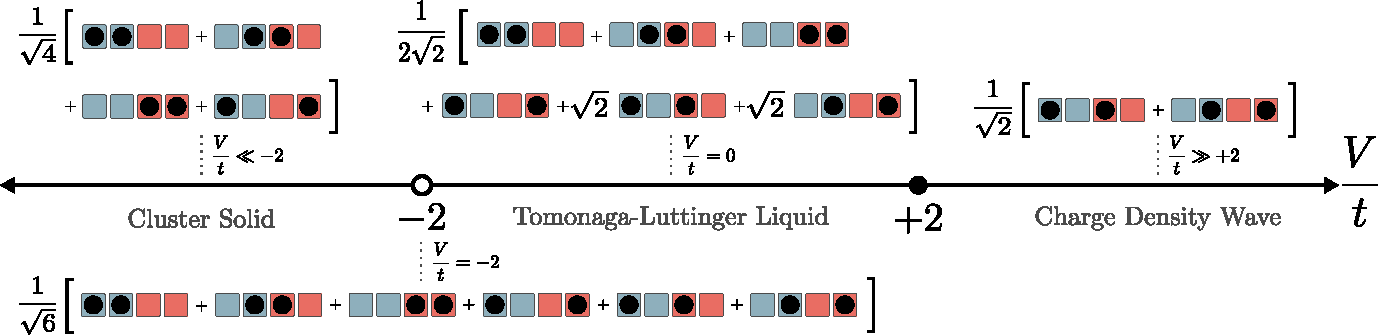
\includegraphics[width=1.0\textwidth]{phaseDiagramTV.pdf}
\end{center}
\caption{Phase diagram of the $t-V$ model accompanied by pictures of candidate ground states for $N=2$ fermions on a $L=4$ site lattice. For the purposes of measuring accessible entanglement, the lattice has been bipartitioned into spatial subregions $A$ (blue) and $B$ (red), each of size $\ell = 2$. We assume periodic boundary conditions. In the limit of strong attractive interactions where $V/t \ll -2$, the particles cluster together and there are $L$ equally probable configurations corresponding to all translations of the cluster.  At the first order phase transition where $V/t = -2$, all ${L}\choose{N}$ configurations are equally probable resulting in a flat state. In the TLL phase with $|V/t| < 2$,  particles are delocalized and we have included a characteristic state corresponding to free fermions $(V=0)$. In the limit of strong repulsive interactions where $V/t \gg 2$, fermions maximize their distance from each other resulting in a charge density wave (CDW) phase. The open and closed circles on the $V/t$ axis denote a first order and continuous phase transition, respectively.}
\label{fig:phaseDiagram}
\end{figure*}
%%%%%%%%%%%%%%%%%

Figure \ref{fig:phaseDiagram} shows the phase diagram of the $tV$ model. For $V/t \ll -2$, the fermions cluster together due to the strong attractive interaction. The state in this regime is an equal superposition of all possible such cluster configurations over all lattice sites. At $V/t = -2$, the system undergoes a second order phase transition into the Tomonaga-Luttinger Liquid (TLL) phase. Here, the state is in a superposition of all possible configurations of the fermions on the lattice. The weights for these configurations are in general different and can only be exactly known at $V/t = 0$ \cite{PhysRevLett.121.150501}. At $V/t = 2$, the system undergoes a continuous phase transition into the charged density wave (CDW) phase. At $V/t \gg 2$, the strong repulsion between particles leads to them forming an alternating pattern of particle-vacancy-particle-vacancy \dots The state in this regime becomes an equal superposition of the only two possible such configurations.

Notice that in Figure \ref{fig:phaseDiagram} the lattice sites have two different colors, blue and red. This is to illustrate that a system can be partitioned into smaller subregions. In this particular example, each partition would be of size 2 lattice sites. In fact, subdividing a system into this smaller subsystems will be necessary for the main phenomenon of interest in this thesis: quantum entanglement. The bulk of this work will consist on quantifying the amount of entanglement of a system via entropy measures. Before getting to explaining entanglement, in the next section, an overview of entropy or information measures will be given.

\section{Information measures}
\label{sec:informationMeasures}

	The probabilistic nature of quantum mechanics, provides an ideal test bed for entropy measures. In section \ref{sec:tvIntro}, it was mentioned that knowing something about $A$, will give you information about its entangled pair $B$. The amount of information gained in such measurement can be quantified by the entropy of the system. Recall that, in essence, entropy is a measure directly proportional to the disorder of a system. Thus, doing a measurement on a high entropy state, will give more information than in a highly ordered state, in which the outcome of the measurement is more like to be known a priori. For this reason, these will be referred to as information of this work for the remainder of this work.
	
	In this section, the information measure from which the ones that will be used to quantify entanglement will be introduced. Then, the actual measures of entanglement will be presented.
	
	\subsection{Shannon entropy}
	
	The Shannon or information entropy is the average amount of information gained from a a data set in which the entries occur according to some probability distribution. It is defined as:
	%
	\begin{equation}
	S = -\sum_{i} p_i \log_{b} p_i
	\label{eq:shannonEntropy}
	\end{equation}
	%
	where the sum is carried over all entries in the data set and $p_i$ is the probability of measuring entry $i$. The base $b$ can be chosen arbitrarily depending on the context. The base will be chosen as the number $e$ such that $\log_b \to \ln$ for the remainder of this work. Up next, a common day example will be presented in order to give some intuition about how information gain can be estimated with Eq.~\eqref{eq:shannonEntropy}
	
	Consider a regular coin flip. Disregarding all physical effects that can somehow bias the outcome, it is expected that either heads or tails will randomly be with equal probability $1/2$. Then, since there is no bias towards any of the two possible outcomes of the coin flip, the information gain should be at a maximum. The Shannon entropy for this case is:
	%
	\begin{align}
	S &= -\frac{1}{2} \ln{\frac{1}{2}} - \frac{1}{2} \ln{\frac{1}{2}}  \nonumber\\
	&= \ln{2}  \nonumber \\
	S &\approx 0.6931 \nonumber \dots
	\end{align}
	Now, consider a coin that has been modified in such a way that it is more likely to get one outcome than the other. For the sake of this example, let's say that heads shall occur with probability $2/3$, while tails with $1/3$. Then, since it is two times more likely that heads will occur instead of tails, more certainty about the outcome is known beforehand and thus the information gained decreases. Shannon entropy gives:
	%
	\begin{align}
	S &= -\frac{2}{3} \ln{\frac{2}{3}} - \frac{1}{3} \ln{\frac{1}{3}} \nonumber \\
	S &\approx 0.6365 \dots \nonumber
	\end{align}
	%
	Finally, an extreme case would be a coin that was incorrectly manufactured and has heads on two sides. Opposite to a regular coin, in which maximum information is gained because both heads and tails have the same probability, the probability for heads to land in this case is 1, while 0 for tails. Since the result is already known before the coin flip, the information gain after the coin flip is none. Shannon entropy gives:
	%
	\begin{align}
	S &= -1\ln{1} = 0 \nonumber
	\end{align}
	%	

	Now that some intuitive examples were discussed, the quantum information theory counterpart of Shannon's entropy will be presented.
	
	\subsection{von Neumann entropy}
	
	In quantum statistical mechanics, the probabilities of measuring a state are encoded within its density matrix. The density matrix is defined as:
	%
	\begin{align}
	\label{eq:densityMatrix}
	\rho = \vert \Psi \rangle \langle \Psi \vert
	\end{align}
	%
	In quantum information theory, Shannon entropy maps to the von Neumann entropy:
	%
	\begin{equation}
	S = -\Tr\rho_{A} \ln{\rho_A}
	\label{eq:vonNeumannEntropy}
	\end{equation}
	%
	where $\rho_A$ is the reduced density matrix of subsystem $A$. The reduced density matrix of $A$ is obtained by tracing out the degrees of freedom of $B$:
	%
	\begin{equation}
	\rho_{A} = \Tr_B \rho = \sum_b \langle \psi_b \vert \Psi \vert \psi_b \rangle
	\label{eq:partialTrace}
	\end{equation}
	%
	where the sum is carried over all possible states in which subsystem $B$ can be in.
	
	\subsection{R\'enyi entropy}

	
\section{Quantum entanglement}
\label{sec:quantumEntanglement}

	A quantum many body system is entangled if its constituents present correlations that cannot be classically described. In other words, assuming subsystems $A$ and $B$ are entangled with one another, knowing something about $A$ automatically gives you some knowledge of $B$. These subsystems can represent subsets of particles, spatial subregions, or just some quantum mode in general, such as momentum. An overview of each of these type of partitions will now be given.

	\subsection{Particle entanglement}
	
	The particles of a quantum many body system can be given labels, such that subsets of particles in the system that share a common label can be considered as a subsystem. Then, the particle partitioned entanglement can be quantified. 
	
	Mathematically,  if a system is entangled or not can be determined by rewriting the state of the system in terms of the states of each subsystem $A$ and $B$. If the overall state cannot be factored into tensor products of the states of $A$ and $B$, then the system is entangled. The condition for entanglement of $A$ and $B$ is then:
	
	\begin{equation}
	\vert\Psi\rangle \neq \vert\Psi_{A}\rangle \otimes \vert\Psi_{B}\rangle
	\label{eq:entanglementCondition}
	\end{equation}
	
	$\vert\Psi_{A}\rangle$ and $\vert\Psi_{B}\rangle$ represent the states of subsystems $A$ and $B$, respectively. Formally, the state $\vert\Psi_{A}\rangle$ is a vector space that exists in Hilbert Space $A$, and likewise for $B$, such that the full Hilbert Space of the system is a tensor product of the subspaces: $\mathcal{H} = A \otimes B$.
	
	Due to the indistinguishability of particles, the $n$-body reduced of the ........
	
	\begin{equation}
	\rho_{n} = \int dx_n \dots \int dx_1 \langle x_1 \dots x_n \vert\Psi\rangle \langle\Psi\vert x_1 \dots x_N \rangle
	\label{eq:nBodyDensityMatrix}
	\end{equation}
	
	
 	
	\subsection{Spatial and mode entanglement}
	
	\subsection{Accessible Entanglement}



	

	


\chapter{Particle Partition Entanglement in the $tV$ Model}
\section{The operational entanglement}

Consider some $N$-particle quantum state, in which the $N$ particles are shared between spatial subregions $A$ and $B$, or Alice and Bob, if you will. If Alice's and Bob's particles are entangled, this entanglement could be used as a resource for real world applications. Nevertheless, by using the traditional Von Neumann or R\'enyi Entanglement entanglement entropy, an overestimated measure of the physically available entanglement is obtained. This happens because for applications that rely on quantum entanglement, the particle number has to be conserved and these traditional measures do not account for this. To address this issue, Wiseman and Vaccaro \cite{PhysRevLett.91.097902} developed a measure known as Operational Entanglement (originally called Entanglement of Modes by the authors). The operational entanglement takes into account that the local particle number that are in Alice and Bob has to be conserved, giving a more physically accurate measure of entanglement.

	\subsection{Projecting onto subspaces of fixed local particle number}
	
	Knowing the density matrix of subregion $A$ will suffice to calculate, for example, the spatial R\'enyi Entanglement Entropy. Nevertheless, to get the operational entanglement, simply knowing $\rho_{A}$ is not enough. To recap, the spatial R\'enyi Entanglement Entropy is given by:
	

\begin{equation}
 S_{\alpha}(\rho_{A}) = \frac{1}{1-\alpha} \log{\Tr{\rho_{A}^{\alpha}}} 
\end{equation}

Where $\alpha$ is the R\'enyi Index and $\rho_{A}$ is the density matrix of subregion $A$. This calculation is still required to get operational entanglement but, as shall be seen, a few extra steps have to be taken to make sure that local particle number conservation is being satisfied. The first of these extra steps will be to project $\rho_{A}$ to subspaces of local particle number. Projection operators can be written as diagonal matrices with ones on the columns corresponding to the subspace for which the projection is desired. Knowing this, the projection operators into subspaces of fixed local particle numbers can be built rather simply. The projected reduced density matrix of  $A$ into the subspace of fixed local particle number $n$ is obtained by:

\begin{equation}
\rho_{A,n} = \frac{1}{P_n} \hat{\Pi}_n \rho_A \hat{\Pi}_n
\end{equation}

Where $P_n$ is the probability of measuring an Alice state with $n$ particles and $\hat{\Pi}_{n}$ is the projection operator onto the subspace of local particle number $n$.

After all this preamble, the operational entanglement can now be obtained. The operational entanglement is:

\begin{equation}
S_{\alpha}^{op}(\rho_A) = \sum_{n} P_n S(\rho_{A,n}) 
\end{equation}

Where the sum is carried over all possible local particle numbers that Alice may have. In other words, $n=0,1,...,N-n_{B}$.

In the following section, analytical results of the operational entanglement entropy at differential interaction strength regimes in the $tV$ model are derived.


\section{Analytical results at various regimes of the $tV$ model}
	In the $tV$ model, the state of the system is exactly known in three different interaction strength regimes:
	
	\begin{enumerate} [i)]
		%\item Charged Density Wave (CDW): $V/t \to +\infty $
		%\item Phase Separated Solid:  $V/t \to +\infty $
		%\item First Order Phase Transition: V/t = -2
		
		\item$V/t \to +\infty $
		\item $V/t \to +\infty $
		\item $V/t = -2$
	\end{enumerate}
	
	Starting from the known states at these regimes, analytical values for the operational entanglement were calculated. The results will be discussed in this section.

	\subsection{Infinitely repulsive interaction}
		The state in this limit is known as a charged density wave (CDW). In the occupation number basis, the CDW state is:

\[| \Psi \rangle_{CDW} = \frac{1}{\sqrt{2}} [|101010... \rangle + |010101... \rangle ] \]

Where $1$ denotes that the site is occupied and $0$, that it is vacant. The coefficient before the bracket is a normalization constant. As will be shown, the operational entanglement for this state is dependent on the parity of the total number of particles $N$. Up next, the result for even N will be derived.

\begin{samepage}
	\subsubsection{Even N}
	In the following calculations, again, the system will be partitioned into spatial subregions $A$ and $B$, both containing the same number of sites. In other words, if the total number of sites in the $t-V$ chain is $L$, then the partition size will be $l=\frac{L}{2}$. \\
	
In the case of even particle number N, the CDW state will have the same number of particles in each subregion $A$ and $B$:

\begin{equation}
| \Psi \rangle_{N_{Even}} = \frac{1}{\sqrt{2}} [|\underbrace{1010...}_{\frac{N}{2} particles}, \underbrace{1010...}_{\frac{N}{2} particles} \rangle + |\underbrace{0101...}_{\frac{N}{2} particles}, \underbrace{0101...}_{\frac{N}{2} particles} \rangle ] 
\end{equation}

As a reminder, labels left to the comma correspond to spatial subregion $A$, while those to the right correspond to $B$.

The full density matrix $\rho_{AB}$ takes the form:

\begin{equation}
\begin{aligned}
\rho_{AB} &= | \Psi \rangle_{N_{Even}} \langle \Psi |_{N_{Even}} \\
&= \frac{1}{2} |0101...,0101\rangle \langle 0101...,0101... | + \frac{1}{2} |0101...,0101\rangle \langle 1010...,1010... |  \\
&+ \frac{1}{2} |1010...,1010\rangle \langle 0101...,0101... | + \frac{1}{2} |1010...,1010\rangle \langle 1010...,1010... |  \\
\end{aligned}
\end{equation}

Recall that to calculate the entanglement entropies, it is necessary to obtain the reduced density matrix of subsystem $A$. Taking the partial trace with respect to $B$, the reduced density matrix of $A$ is obtained:

\begin{equation}
\begin{aligned}
\rho_{A} &= \Tr_{B} \rho_{AB} &= \sum_{n} {}_B \langle n | \Psi \rangle \langle \Psi | n \rangle_{B} \\
\end{aligned}
\end{equation}

Where the summation is carried over all possible states that $B$ can be found in. In this case, there are only two possible $B$ states: $n = |0101...\rangle_{B}$ and $|1010...\rangle_{B} $Thus, taking the partial trace respect to $B$ of Eq. $(2.5)$:

\begin{equation}
\begin{aligned}
\rho_{A} &= \frac{1}{2} | 0101... \rangle_{A} \langle 0101... |_{A} +  \frac{1}{2} | 1010... \rangle_{A} \langle 1010... |_{A} \\
\end{aligned}
\end{equation}

Notice that some of the terms have vanished due to the orthonormality of the states. At this point, it will be convenient for purposes of illustration to rewrite the reduced density matrix of $A$ in actual matrix form rather than in Dirac or Bra-Ket notation:

\begin{equation}
\begin{aligned}
\rho_{A} &= \begin{pmatrix}
\frac{1}{2} & 0 \\
0 & \frac{1}{2} \\
\end{pmatrix} \\
\end{aligned}
\end{equation}

For spatial entanglement, $\rho_{A}$ would suffice, but for operational entanglement, the matrix has to be projected onto the various subspaces of fixed local particle number in $A$. In this case, both of the states share the same local particle number. That is, the states: $|1010...\rangle_{A}$ and $|0101...\rangle_{A}$ both have local particle number $n = \frac{N}{2}$. Thus only one projection operator is needed. In fact, the operator needed here turns out to be equal to the identity operator:


\begin{equation}
\begin{aligned}
\hat{\Pi}_{n={\frac{N}{2}}} = \begin{pmatrix} 
1&0 \\
0&1 \\
\end{pmatrix} = \hat{I}
\end{aligned}
\end{equation}

The probability of measuring a state with local particle number $n = \frac{N}{2} $ is equal to one. Thus, the projected density matrix of $A$ onto the subspace of $n=\frac{N}{2}$ is:

\begin{align} \rho_{A,\frac{N}{2}} &= \frac{1}{P_{\frac{N}{2}}} \hat{\Pi}_{\frac{N}{2}} \rho_{A} \hat{\Pi}_{\frac{N}{2}} \\ 
& = \hat{I} \rho_{A} \hat{I}  \\
\rho_{A,\frac{N}{2}} &= \rho_{A} = \begin{pmatrix} \frac{1}{2}&0 \\ 0&\frac{1}{2} \end {pmatrix} 
\end{align}

The reduced, projected and normalized reduced density matrix of $A$ is now known and can be substituted into Eq. $2.3$ to calculate the operational entanglement entropy:
\begin {align} 
S_{\alpha}^{op}(\rho_A) &= \sum_{n} P_n S_{\alpha}(\rho_{A,n}) \\
&= \frac{1}{1-\alpha} \log{\Tr{\rho_{A,\frac{N}{2}}^{\alpha}}} \\
&= \frac{1}{1-\alpha} \log{\Tr{\begin{pmatrix}  (\frac{1}{2})^{\alpha} & 0 \\ 0 & (\frac{1}{2})^{\alpha}   \end{pmatrix}}} \\
&= \frac{1}{1-\alpha} \log({\frac{1}{2^{\alpha}} + \frac{1}{2^{\alpha}}}) \\
&= \frac{1}{1-\alpha} \log{2^{(1-\alpha)}} \\
S_{\alpha}^{op}(\rho_A) &= \log{2}
\end {align}

Thus, for even $N$ and $V/t \to + \infty$ , the operational entanglement converges to $\log{2}$. Up next, the result for odd $N$ will be derived.

	\subsubsection{Odd N}
	
	The most general quantum state becomes:
	
	\begin{equation}
	| \Psi \rangle_{N_{Odd}} = \frac{1}{\sqrt{2}} [|\underbrace{...101}_{\frac{N+1}{2} particles}, \underbrace{010...}_{\frac{N-1}{2} particles} \rangle + |\underbrace{...010}_{\frac{N-1}{2} particles}, \underbrace{101...}_{\frac{N+1}{2} particles} \rangle ]
	\end{equation}
	
	Note that now when doing an equal spatial bipartition, one of the subregions will have one more particle than the other, unlike the even particle case in which both subregions had the same number of particles. Specifically, one of the subregions will have $\frac{N+1}{2}$ and the other, $\frac{N-1}{2}$. This implies that $\rho_{A}$ will have to be projected onto the space of local particle number $\frac{N+1}{2}$ and $\frac{N-1}{2}$. But before doing that, again the full body density matrix is needed:
	
	\begin{equation}
	\begin{aligned}
\rho_{AB} &= | \Psi \rangle_{N_{Even}} \langle \Psi |_{N_{Even}} \\
&= \frac{1}{2} |...101,010... \rangle \langle ...101,010... | + \frac{1}{2} |...101,010... \rangle \langle ...010,101... |  \\
&+ \frac{1}{2} |...010,101... \rangle \langle ...101,010... | + \frac{1}{2} |...010,101... \rangle \langle ...010,101... |  \\
	\end{aligned}
	\end{equation}
	
The possible $B$ states are: $n = | 101... \rangle, | 010... \rangle$ with $\frac{N+1}{2}$ and $\frac{N-1}{2}$ particles, respectively. Taking the partial trace respect to B, the reduced density matrix of $A$ becomes:
	
	\begin{equation}
\begin{aligned}
\rho_{A} &= \frac{1}{2} | 101... \rangle_{A} \langle 101... |_{A} +  \frac{1}{2} | 010... \rangle_{A} \langle 010... |_{A} \\
\end{aligned}
\end{equation}

Once again, it may be more illustrative to rewrite in matrix form. Defining an orthonormal basis $| 101... \rangle_{A}  = \begin{pmatrix} 1 \\ 0\end{pmatrix}$ and $| 010... \rangle_{A}  = \begin{pmatrix} 0 \\ 1\end{pmatrix}$ the reduced density matrix of $A$ becomes:

\begin{equation}
\rho_{A} = 
\begin{pmatrix}
\frac{1}{2} & 0 \\
0 & \frac{1}{2}
\end{pmatrix}
\end{equation}

The simple projection operators onto $\frac{N+1}{2}$ and $\frac{N-1}{2}$ particle space in this basis are:

\begin{equation}
\hat{\Pi}_{\frac{N+1}{2}} = \begin{pmatrix} 1 & 0 \\ 0 & 0 \end{pmatrix} , 
\hat{\Pi}_{\frac{N-1}{2}} = \begin{pmatrix} 0 & 0 \\ 0 & 1 \end{pmatrix} 
\end{equation}

Applying these projections to $\rho_{A}$ and choosing the probability such that the trace of each matrix is unity (normalization):

\begin{equation}
\rho_{A,{\frac{N+1}{2}}} = \begin{pmatrix} 1 & 0 \\ 0 & 0 \end{pmatrix}  \text{ with probability } P_{\frac{N+1}{2}} = \frac{1}{2}
\end{equation}

and 

\begin{equation}
\rho_{A,{\frac{N-1}{2}}} = \begin{pmatrix} 0 & 0 \\ 0 & 1 \end{pmatrix}  \text{ with probability } P_{\frac{N-1}{2}} = \frac{1}{2}
\end{equation}

Substituting into the operational entanglement equation (Eq. 2.3):

\begin {align} 
S_{\alpha}^{op}(\rho_A) &= \sum_{n} P_n S_{\alpha}(\rho_{A,n}) \\
&= (\frac{1}{2})\frac{1}{1-\alpha} \log{\Tr{\rho_{A,\frac{N+1}{2}}^{\alpha}}} + (\frac{1}{2})\frac{1}{1-\alpha} \log{\Tr{\rho_{A,\frac{N-1}{2}}^{\alpha}}} \\
&=\frac{1}{2-2\alpha}[ \log{\Tr{\begin{pmatrix}  1^{\alpha} & 0 \\ 0 & 0   \end{pmatrix}}} + \log{\Tr{\begin{pmatrix}  0 & 0 \\ 0 & 1^{\alpha}   \end{pmatrix}}}]\\
&=  \frac{1}{2-2\alpha}[ \underbrace{\log{1} + \log{1}}_{=0} ]\\
S_{\alpha}^{op}(\rho_A) &= 0
\end {align}

Therefore, the operational entanglement vanishes in the infinite repulsion limit ($V/t \to + \infty$) and odd number of particles in the system.

Summarizing:

\begin{equation}
\lim_{V \to + \infty} S_{\alpha}^{op} =
\begin{cases}
\log{2}  & \text{if }N\text{ is even} \\
0 & \text{if }N\text{ is odd}
\end{cases}
\end{equation}

\end{samepage}

	\subsection{Infinitely attractive interaction}
	In this section, an analytical result will be derived at half-filling ($L = 2N$) and partition size equal to the half the number of sites ($\ell = \frac{L}{2}$) for $V/t \to - \infty$. After arriving to the half-filling result, a general result, for any filling fraction and partition size, will be also derived. 
	
	\subsubsection{Half-filling}
	In the infinitely attractive regime of the $tV$ model, $V/t \to -\infty$, the fermions cluster together. The most general state in this regime is:
	
\begin{equation}
\begin{aligned}	
| \Psi \rangle_{PSS} = \frac{1}{\sqrt{L}} [ | \underbrace{111...111}_{N particles} , \underbrace{000...000}_{N vacancies} \rangle + |011...111, 100...000 \rangle + |001...111, 110...000 \rangle  \\
+ ...  + |\underbrace{000...000}_{N vacancies}, \underbrace{111...111}_{N particles} \rangle + |100...000, 011...111 \rangle + ... |111...110, 000...001 \rangle ]
\end{aligned}
\end{equation}

This state is known as a phase separated solid (PSS). There are a total of $L$ possible configurations, hence the normalization constant $\frac{1}{\sqrt{L}}$. 

In an effort to simplify the notation while keeping the calculation general, the $A$ or $B$ states will be relabeled as:

\begin {align*}
&| 111...111 \rangle \to | N \rangle \\
&| 011...111 \rangle \to | N-1 \rangle \\
&| 001...111 \rangle \to | N-2 \rangle \\
&\vdots \\
&| 000...011 \rangle \to | 2 \rangle \\
&| 000...001 \rangle \to | 1 \rangle \\
&| 000...000 \rangle \to | 0 \rangle 
\end {align*}

There is still one flaw with this notation. A $| N-1 \rangle $ state could represent either $| 011...111 \rangle $ or $|111...110 \rangle $. In other words, even though they have the same local particle number $N-1$, the configurations themselves are different. One way in which this problem can be circumvented is by adding a subscript to the label to represent distinct configurations. Since particle number will only be shared between two distinct particle configurations, using subscripts of $1$ and $2$ seems natural. For example: $| 011...111 \rangle \to | (N-1)_1 \rangle$ and $|111...110 \rangle \to | (N-1)_2 \rangle$. $|\Psi\rangle_{PSS}$ now becomes:

\begin{equation}
| \Psi \rangle_{PSS} = \frac{1}{\sqrt{L}} [ |N, 0 \rangle + |(N-1)_1, 1_1 \rangle + |(N-2)_1, 2_1 \rangle  
+ ...  + |0, N \rangle + |1_2, (N-1)_2 \rangle + ... |(N-1)_2, 1_2 \rangle ]
\end{equation}

Taking the outer product of Eq. $2.33$ with itself, the full body density matrix is obtained:

\begin{equation}
\rho_{AB} = | \Psi \rangle_{PSS} \langle \Psi |_{PSS} = 
\begin{pmatrix} 
\frac{1}{L} & \frac{1}{L} & ... & \frac{1}{L} \\
\frac{1}{L} & \frac{1}{L} & ... & \frac{1}{L} \\
\vdots & \vdots & \vdots & \vdots \\
\frac{1}{L} & \frac{1}{L} & ... & \frac{1}{L} \\
\end{pmatrix}
\end{equation}

The full body density matrix is of size $LxL$ with all entries equal to $\frac{1}{L}$. Before proceeding, the basis of this matrix should be described. Columns (from left to right) and rows (from top to bottom) are arranged as: \\ $| N, 0 \rangle , |0, N \rangle , | (N-1)_1, 1_1 \rangle, |(N-1)_2, 1_2 \rangle , | (N-2)_1, 2_1 \rangle , | (N-2)_2, 2_2 \rangle , ... , \\ |2_1, (N-2)_1 \rangle , \rangle, |2_2, (N-2)_2 \rangle , \rangle, |1_1, (N-1)_1 \rangle , \rangle, |1_2, (N-1)_2 \rangle  $ . Notice that configurations that share local particle number have been paired up next to each other. The first two states are exceptions, as their subregions never share the same local particle number with subregions of any other state. Now that the basis has been explained, it's time to get the reduced density matrix of $A$. \\
\\
Taking the partial trace with respect to $B$ of Eq. $2.34$:

\begin{equation}
\rho_{A} = \begin{pmatrix}
\frac{1}{L} & 0 &... & 0 & 0 \\
0 & \frac{1}{L} & ... & 0 & 0 \\
\vdots & \vdots & \ddots & \vdots & \vdots \\
0 & 0 & ... & \frac{1}{L} & 0 \\
0 & 0 & ... & 0 & \frac{1}{L} \\
\end{pmatrix}
\end{equation}

And in the hopes of being as explicit as possible, the rows and columns correspond to the following configurations and in the following order: $| N \rangle , |0 \rangle , | (N-1)_1 \rangle, |(N-1)_2 \rangle , | (N-2)_1 \rangle , | (N-2)_2 \rangle , ... , |2_1 \rangle , |2_2 \rangle , |1_1 \rangle , |1_2 \rangle $ 

Now, $\rho_{A}$ has to be projected onto the subspaces of local particle numbers. The allowed local particle numbers are: $n = N, N-1, N-2 .... 2, 1, 0$. So a total of $\frac{M}{2} + 1$ projections need to be done. There is a projection onto the subspace of $n = 0$, one onto $n = N$ and $\frac{M}{2} -1$ onto the remaining subspaces. The $\frac{M}{2}$ was obtained due to the pairs of states that share local particle number: $|(N-1)_1 \rangle \text{ with } |(N-1)_2 \rangle, |(N-2)_1 \rangle \text{ with } |(N-2)_2 \rangle$ and so on and so forth. The $1$ is subtracted because the pair of states $| 0 \rangle$ and $| N \rangle$ don't share local particle number.

The projection operators for $n=0$ and $n=N$ become:

\begin{equation}
\hat{\Pi}_{N} = \begin{pmatrix} 
1 & 0 &... & 0 & 0 \\
0 & 0 & ... & 0 & 0 \\
\vdots & \vdots & \ddots & \vdots & \vdots \\
0 & 0 & ... & 0 & 0 \\
0 & 0 & ... & 0 & 0 \\
\end{pmatrix} , 
\hat{\Pi}_{0} = \begin{pmatrix} 
0 & 0 &... & 0 & 0 \\
0 & 1 & ... & 0 & 0 \\
\vdots & \vdots & \ddots & \vdots & \vdots \\
0 & 0 & ... & 0 & 0 \\
0 & 0 & ... & 0 & 0 \\
\end{pmatrix}
\end{equation}

For the remaining $\frac{M}{2} - 1$ states, there will be two consecutive non-zero entries in the diagonal. For example:

\begin{equation}
\hat{\Pi}_{N-1} = \begin{pmatrix} 
0 \\
& 0 \\
& & 1 \\
& & & 1 \\
& & & &  0 \\
& & & & & 0 \\
& & & & &  & \ddots \\
& & & & & & &  0 \\
& & & & & & & &  0 \\
\end{pmatrix}
\end{equation}

\begin{equation}
\hat{\Pi}_{N-2} = \begin{pmatrix} 
0 \\
& 0 \\
& & 0 \\
& & & 0 \\
& & & &  1 \\
& & & & & 1 \\
& & & & &  & \ddots \\
& & & & & & &  0 \\
& & & & & & & &  0 \\
\end{pmatrix}
,
\hat{\Pi}_{1} = \begin{pmatrix} 
0 \\
& 0 \\
& & 0 \\
& & & 0 \\
& & & &  0 \\
& & & & & 0 \\
& & & & & & \ddots \\
& & & & & & &  1 \\
& & & & & & & &  1 \\
\end{pmatrix}
\end{equation} \\
\\
Notice from the form of the projection operators that the projected reduced density matrices will be similar to each other but with the two non-zero entries shifted correspondingly in the diagonal. Thus taking the projection onto $n=N-1$ of $\rho_{A}$:

\begin{equation}
\begin{aligned}
\rho_{A,N-1} &= \frac{1}{P_{N-1}} \hat{\Pi}_{N-1} \rho_{A} \hat{\Pi}_{N-1} \\
\rho_{A,N-1} &= \frac{1}{P_{N-1}} \begin{pmatrix} 
0 \\
& 0 \\
& & \frac{1}{L} \\
& & & \frac{1}{L} \\
& & & &  0 \\
& & & & & 0 \\
& & & & &  & \ddots \\
& & & & & & &  0 \\
& & & & & & & &  0 \\
\end{pmatrix} 
\end{aligned}
\end{equation}

The probability of measuring a state with local particle number $N-1$ can be obtained from normalization:

\begin{equation}
\Tr{\rho_{A,N-1}} = 1 \implies \frac{1}{P_{N-1}}\frac{2}{L} = 1 \implies P_{N-1} = \frac{2}{L}
\end{equation}

Thus the projection onto $n=N-1$ of $\rho_{A}$ is:

\begin{equation}
\rho_{A,N-1} = \begin{pmatrix} 
0 \\
& 0 \\
& & \frac{1}{2} \\
& & & \frac{1}{2} \\
& & & &  0 \\
& & & & & 0 \\
& & & & &  & \ddots \\
& & & & & & &  0 \\
& & & & & & & &  0 \\
\end{pmatrix} ; \text{ with probability } P_{N-1} = \frac{2}{L}
\end{equation}

For $n = N-2$:
\begin{equation}
 \rho_{A,N-2} = \begin{pmatrix} 
0 \\
& 0 \\
& & 0  \\
& & & 0 \\
& & & &  \frac{1}{2} \\
& & & & & \frac{1}{2} \\
& & & & &  & \ddots \\
& & & & & & &  0 \\
& & & & & & & &  0 \\
\end{pmatrix} ; \text{ with probability } P_{N-2} = \frac{2}{L}
\end{equation}

and so on and so forth. \\
\\
Similarly, $\rho_{A,N}$ and $\rho_{A,0}$ become:
\begin{equation}
\rho_{A,N} = \begin{pmatrix} 
1 \\
& 0 \\
& & 0  \\
& & & 0 \\
& & & &  0 \\
& & & & & 0 \\
& & & & &  & \ddots \\
& & & & & & &  0 \\
& & & & & & & &  0 \\
\end{pmatrix} ,
\rho_{A,0} = \begin{pmatrix} 
0 \\
& 1 \\
& & 0  \\
& & & 0 \\
& & & &  0 \\
& & & & & 0 \\
& & & & &  & \ddots \\
& & & & & & &  0 \\
& & & & & & & &  0 \\
\end{pmatrix} 
\end{equation}

with probabilities $P_{N} = P_{0} = \frac{1}{L}$

Finally, the operational entanglement is:

\begin{align} 
S_{\alpha}^{op}(\rho_A) &= \sum_{n} P_n S_{\alpha}(\rho_{A,n}) \\
&= \frac{1}{1-\alpha}[\frac{1}{L} \log{\Tr{\rho_{A,N}^\alpha}} + \frac{1}{L} \log{\Tr{\rho_{A,0}^\alpha}} + \frac{2}{L} \log{\Tr{\rho_{A,N-1}^\alpha}}  \\
&+ \frac{2}{L} \log{\Tr{\rho_{A,N-2}^\alpha}} + \dots +\frac{2}{L} \log{\Tr{\rho_{A,2}^\alpha}} + \frac{2}{L} \log{\Tr{\rho_{A,1}^\alpha}} ] \\
&= \frac{1}{L-L\alpha}[ \underbrace{\log{1}}_{=0} +  \underbrace{\log{1}}_{=0} + 2 \log({\frac{1}{2^\alpha}+\frac{1}{2^\alpha}}) \\
&+ 2 \log({\frac{1}{2^\alpha}+\frac{1}{2^\alpha}})+ \dots + 2 \log({\frac{1}{2^\alpha}+\frac{1}{2^\alpha}}) + 2 \log({\frac{1}{2^\alpha}+\frac{1}{2^\alpha}}) ] \\
&= \frac{2}{L-L\alpha}\underbrace{[\log{2^{(1-\alpha)}} + \log{2^{(1-\alpha)}} + \dots + \log{2^{(1-\alpha)}} + \log{2^{(1-\alpha)}}}_{\frac{L}{2} - 1 \text{ terms }}] \\
&= (\frac{L}{2}-1)(\frac{2}{L})\log{2^\frac{1-\alpha}{1-\alpha}} \\
&= (\frac{L-2}{2})(\frac{2}{L})\log{2} ; \text{ recall that } L = 2N \\
S_{\alpha}^{op}(\rho_A) &= \frac{N-1}{N}\log{2}
\end{align}

\subsubsection{Analytical result for any filling fraction and partition size}

The analytical result obtained above for the operational entanglement entropy in the infinitely attractive regime corresponds to the special case of half-filling ($N = \frac{L}{2}$) and equal spatial bipartitions ($\ell_{A} = \ell_{B} = \frac{L}{2}$). Nevertheless, a generalized result can be obtained for ant filling fraction and partition size by counting the number of projected reduced density matrices ($\rho_{A,n}$) that will contribute to the operational entanglement. As it will be shown, the number of contributing matrices will depend on how the quantities $\ell_{A}, \ell_{B}, N \text{ } \&  \text{ }N^{c} = L-N$ relate to each other. Demonstration of the following cases will suffice to get the general result:

\begin{align}
&i) \ell_{A} < N < \ell_{B} \\
&ii) \ell_{B} < N < \ell_{A} \\
&iii)  N < \ell_{A} < \ell_{B} \\
&iv) \ell_{A} < \ell_{B} < N
\end{align}

These four cases actually imply other cases and, in the end, all possible relations between the four parameters should be covered. \\

Case $i)$ $\ell_{A} < N < \ell_{B}$:

The condition here is that the size of the subregion $A$ should be less than the total number of particles $N$ and the size of the subregion $B$ should be greater than both of these quantities. Under such conditions, particle configurations in which $B$ is empty are not possible, since $A$ is too small too fit them all. Two other configurations that will not contribute to the operational entanglement are when $A$ is full ($n_{A} = \ell_{A}$) and when it is empty ($n_{A} = 0$). There is only one possible way of distributing the particles in partition $A$ if it is full and likewise if it is empty. As it was seen in the previous section, then the corresponding projected reduced density matrices $\rho_{A,\ell_{A}}$ and $\rho_{A,0}$ have only one nonzero eigenvalue which, after normalization, becomes 1. Thus, $\ln \rho_{A,\ell_{A}}^{\alpha} = \ln \rho_{A,0}^{\alpha} = 0$. There are a total of $\ell_{A}+1$ possible local particle numbers ($n_{A}$) and since $n_{A} = \ell_{A}$ and $n_{A} = 0$ do not contribute, there are actually $\ell_{A}-1$ contributing projected reduced density matrices. All such projected density matrix will have the form:

\begin{equation}
\rho_{A,n} = \begin{pmatrix} 

\frac{1}{L} & 0 \\
0 & \frac{1}{L} \\

\end{pmatrix}
\end{equation}

The two diagonal elements come from the two configurations that have the same local particle number $n$. Technically, these projected reduced density matrices originally have the same dimensions as those in Eqs.$2.37-2.39,2.41-2.43$. Nevertheless, rows and columns that only have zero entries have been thrown out for compactness. Normalizing:

\begin{equation}
\rho_{A,n} = \frac{1}{P_n} \begin{pmatrix} 

\frac{1}{2} & 0 \\
0 & \frac{1}{2} \\

\end{pmatrix} ; P_n = \frac{2}{L}
\end{equation}

Thus, the operational entanglement becomes:

\begin{equation}
S_{\alpha}^{op} (\ell_A, L) = (\ell_{A} - 1) \frac{2}{L} \ln{2}
\end{equation}

Case $ii)$ $\ell_{B} < N < \ell_{A}$:

This time, partition $B$ is the one that can never be empty. Barring that, the argument is exactly the same as $i)$ and thus:

\begin{equation}
S_{\alpha}^{op} (\ell_{B}, L) = (\ell_{B} - 1) \frac{2}{L} \ln{2}
\end{equation}

Case $iii)$ $N < \ell_{A} < \ell_{B}$:

In contrast to $i)$ and $ii)$, now the particles may all be in $A$ or all in $B$. Nevertheless, in such instances, there is only a single possible configuration of the other partition, that in which it's empty. Thus, the projected reduced density matrices $\rho_{A,N}$ and $\rho_{A,0}$ have only one nonzero eigenvalue and, thus, do not contribute to the operational entanglement. Barring these two, there are then $N-1$ projected reduced density matrices that do contribute. They all have the same form as the ones of $i)$ and $ii)$, that is, $2x2$ diagonal matrices (after throwing out all unnecessary zeroes) with 2 eigenvalues $\frac{1}{2}$ (after normalizing) and probabilities $P_n = \frac{2}{L}$. Thus:

\begin{equation}
S_{\alpha}^{op} (N, L) = (N - 1) \frac{2}{L} \ln{2}
\end{equation}

Case $iv)$ $\ell_{A} < \ell_{B} < N$:

Here, no partition will ever be empty. The maximum allowed particle number in $A$ is going to be $n_{A} = \ell_{A}$ and the smallest one, $n_{A} = N - \ell_{B}$. The partition size of $B$ is subtracted from $N$ because the minimum $n_A$ corresponds to a fully occupied partition $B$, that is $n_B = \ell_B$. The 'leftover' particles on $A$ will hence be the total particle number minus those fully occupying $B$. Notice in all the previous examples that the total number of projected reduced density matrix is equal to the difference between max and min allowed particle number $n_A$ plus 1. That is:

\begin{equation}
\text{Total Projected Reduced Density Matrices} = (n_A)_{max} - (n_A)_{min} + 1
\end{equation}

And for this case,

 \begin{align}
\text{Total Projected Reduced Density Matrices} &= (n_A)_{max} - (n_A)_{min} + 1 \\
&= \ell_A - (N-\ell_B) + 1 \\
&= \underbrace{\ell_A + \ell_B}_{L} - N + 1 \\
\text{Total Projected Reduced Density Matrices} &= L - N + 1
\end{align}

Let $L-N \equiv N^c$. The total number of contributing projected reduced density matrices is:

\begin{align}
\text{Contributing Matrices} &= \text{Total Matrices} - 2 \\
&= (N^c + 1) - 2 \\
\text{Contributing Matrices} &= N^c - 1 \\
\end{align}

the operational entanglement then becomes:

\begin{equation}
S_\alpha^{op}(N^c,L) = (N^c - 1) \frac{2}{L} \ln{2}
\end{equation}

The operational entanglement at the infinitely attractive regime has now been obtained for conditions $i)-iv)$. Notice that it always has the form:

\begin{equation}
S_\alpha^{op}(x,L) = (x - 1) \frac{2}{L} \ln{2}
\end{equation}

where $x$ could be  $\ell_A, \ell_B, N$ or $N^c$. But how to determine which of these variables to choose? Recalling that $L-N = N^c, L-\ell_A = \ell_B$ and $L-\ell_B = \ell_A$, extra inequalities can be obtained from $i)-iv)$ that relate the four variables:

\begin{align}
& i) \ell_{A} < N < \ell_{B} \implies \ell_{B} > N^c > \ell_{A} \implies \ell_{A} \text{ is the smallest} \\
& ii) \ell_{B} < N < \ell_{A} \implies \ell_{A} > N^c > \ell_{B} \implies \ell_{B} \text{ is the smallest} \\
& iii)  N < \ell_{A} < \ell_{B} \implies N^c > \ell_{B} > \ell_{A} \implies N \text{ is the smallest} \\
& iv) \ell_{A} < \ell_{B} < N \implies \ell_{B} > \ell_{A} > N^c \implies N^c \text{ is the smallest} \\
\end{align}

From the above set of inequalities, note that the smallest between the four variables in each case, also happens to be the variable that is substituted for $x$. Thus, in a more compact form, the generalized operational entanglement at the infinitely attractive regime is:

\begin{equation}
S_\alpha^{op}(x,L) = \frac{2(x-1)}{L} \ln{2} ; \text{ where } x = \min{\ell_A, \ell_B, N, N^c}
\end{equation}

	\subsection{First order phase transition}
	
At $\frac{V}{t} = -2$, the $tV$-Model undergoes a first order phase transition from Luttinger Liquid to Phase Separated Solid. The operational entanglement at this interaction strength vanishes and then suddenly increases and converges to the previously derived limit ($\frac{N-1}{N}\ln{2}$) as the attraction gets stronger. In this section, it will be shown that the operational entanglement vanishes at the first order phase transition.

At $\frac{V}{t}=-2$, and half-filling ($N=\frac{L}{2}$), the state of the system is a equiprobable superposition of all possible configurations. There are a total of ${L}\choose{N}$ possible configurations. Thus, the general state can be written as: 

\begin{equation} 
|\Psi \rangle = \frac{1}{\sqrt{{L}\choose{N}}} \sum_{i=1}^{{L}\choose{N}} | \phi_{i} \rangle
\end{equation}

where $|\phi_{i}\rangle$ denotes a distinct particle configuration and the pre-factor is a normalization constant. Now that the state at $\frac{V}{t}=-2$ is known, the full and, hence, reduced density matrices can be obtained. Up next, their resulting general structure will be discussed.

For simplicity, let $\frac{1}{\sqrt{{L}\choose{N}}} \equiv C$. For particle sub-sectors of $n_A = 0$ and $n_A = N$, the projected reduced density matrices become:

\begin{equation}
\rho_{A,N} = \frac{1}{P_{N}} \begin{pmatrix}
C & \dots & 0 \\ 
\vdots & 0 & \vdots \\
0 & \dots & 0 \\
\end{pmatrix}
\end{equation}

with probability $P_{N} = C$. And, 

\begin{equation}
\rho_{A,0} = \frac{1}{P_{0}} \begin{pmatrix}
0 & \dots & 0 \\ 
\vdots & 0 & \vdots \\
0 & \dots & C \\
\end{pmatrix}
\end{equation}

also with probability $P_{0} = C$.

For particle number sub-sectors of $1 \leq n \leq N-1$, the projected reduced density matrices become square matrices of size $NxN$ with all entries being $NC^2$:

\begin{equation}
\rho_{A,n} = \frac{1}{P_{n}} \begin{pmatrix}
NC^2 & \dots & NC^2 \\ 
\vdots & NC^2 & \vdots \\
NC^2 & \dots & NC^2
\end{pmatrix}
\end{equation}

with probabilities $P_{n}=N(NC^2)=N^2C^2$.

In summary, the normalized projected reduced density matrices are:

\[ \rho_{A,N} = \frac{1}{P_{N}} \begin{pmatrix}
1 & \dots & 0 \\ 
\vdots & 0 & \vdots \\
0 & \dots & 0 \\
\end{pmatrix}, P_{N}=C \]
\[ \rho_{A,0} = \frac{1}{P_{N}} \begin{pmatrix}
0 & \dots & 0 \\ 
\vdots & 0 & \vdots \\
0 & \dots & 1 \\
\end{pmatrix}, P_{0}=C\]
\[ \rho_{A,n} = \frac{1}{P_{n}} \begin{pmatrix}
\frac{1}{N} & \dots & \frac{1}{N} \\ 
\vdots & \frac{1}{N} & \vdots \\
\frac{1}{N} & \dots & \frac{1}{N}
\end{pmatrix}, P_{n}=N^2C^2 \]

Recall the definition of the operational (R\'enyi) entanglement entropy:

\[S_{\alpha}^{op}(\rho_{A}) = \sum_{n} P_{n}S(\rho_{A,n})\]

where $S_{\alpha}(\rho_A) = \frac{1}{1-\alpha} \log{\Tr{(\rho_A^{\alpha})}}$

Expanding the sum:

\[ \begin{aligned} S_{\alpha}^{op}(\rho_{A}) &= P_{0} \log{\Tr{(\rho_{A,0}^{\alpha})}} + \sum_{n=1}^{N-1} P_{n} \log{\Tr{(\rho_{A,n}^{\alpha})}} + P_{N} \log{\Tr{(\rho_{A,N}^{\alpha})}} \\
&= C \log{1} + N^2C^2 \sum_{n=1}^{N-1} \log{N(\frac{1}{N})} + C \log{1} \\
&= N^2C^2 \sum_{n=1}^{N-1} \log{1} \\
S_{\alpha}^{op}(\rho_{A}) &= 0 \\
\end{aligned} \]

Thus, the operational entanglement vanishes at the first order phase transition. \\

Analytical results have been obtained in three regimes of the $tV$ Model, namely: $V/t \to + \infty$, $V/t \to - \infty$ and $V/t = -2$. In the next section, numerical results will be discussed.

\section{Numerical Results}
	\subsection{Operational entanglement as a function of interaction strength}
		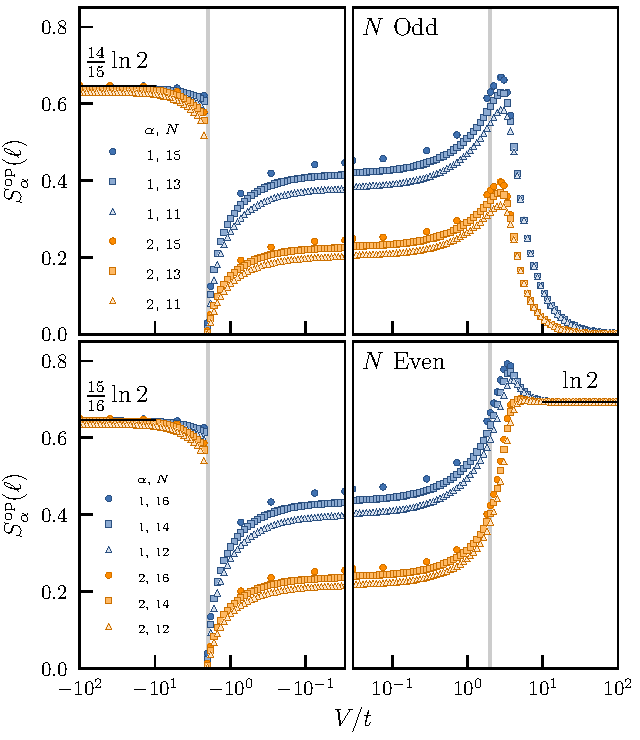
\includegraphics{Images/OperationalEntanglement/operationalEntanglementEntropies}
	\subsection{Scaling of operational entanglement peak}
	
		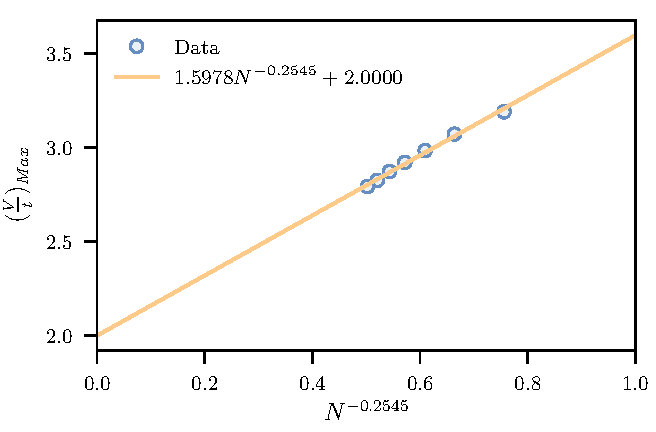
\includegraphics{Images/OperationalEntanglement/peakFitOddN_wLegend}
	\subsection{Entanglement of fluctuations}
	


\chapter{Operationally Accessible Entanglement Entropy in the $tV$ Model}
\section{Operationally Accessible Entanglement Entropy}

\subsection{The \ren Entanglement Entropy}
\label{sec:accEntanglementIntro}

The amount of entanglement that exists between some partition $A$ and its compliment $B$ of a quantum many-body system in pure state $\ket{\Psi}$ can be quantified via the R\'{e}nyi entanglement entropy which depends on an index $\alpha$ :
%
\begin{equation}
S_{\alpha} (\rho_A) = \frac{1}{1-\alpha}\ln \Tr\, \rho_A^{\alpha}
\label{eq:S_alpha}
\end{equation}
%
where $\rho_{A}$ is the reduced density matrix of partition $A$ obtained by
tracing out all degrees of freedom in $B$ from the full density matrix:
%
\begin{equation}
\rho_{A} = \Tr_{B}\, \rho = \Tr_{B} \ket{\Psi}\bra{\Psi}\,.
\end{equation}
%
The \ren entropy is a monotonically decreasing function of $\alpha$ for $\alpha
> 1$ and is bounded from above by the von Neumann entropy, $S_1(\rho_A) = -\Tr \rho_A \ln \rho_A$.

For a quantum many-body system subject to physical laws conserving some quantity (particle number, charge, spin, etc.), the set of local operations on the state $\ket{\Psi}$ are limited to those that don't violate the corresponding global superselection rule.  For the remainder of this paper, we will focus on our discussion on the case of fixed total $N$ and thus we are restricted to only those operators which locally preserve the particle number in $A$.  The effect this has on the amount of entanglement that can be transferred to a qubit register is apparent from the simple example (adapted from Ref.~\cite{Wiseman:2003vn} of one particle confined to two spatial modes $A$ and $B$ corresponding to site occupations.  Then, for the state $\ket{\Psi} = \left(\ket{1}_A \otimes \ket{0}_{B} + \ket{0}_A \otimes \ket{1}_{B} \right)/\sqrt{2}$, Eq.~\eqref{eq:S_alpha} gives that $S_1 = \ln 2$. However, this entanglement cannot be transferred to a register prepared in initial state $\ket{0}_R$ via a $\texttt{SWAP}$ gate:
\begin{align*}
    & \texttt{SWAP} \ket{0}_R\otimes\left(\ket{1}_A \otimes
    \ket{0}_{B} + \ket{0}_A \otimes \ket{1}_{B} \right)/\sqrt{2} \\
    &= \frac{1}{\sqrt{2}}\left( \ket{0}_R \otimes \ket{0}_A \otimes
        \ket{1}_{B} + \ket{1}_R \otimes \ket{0}_A \otimes
    \ket{0}_{B} \right)
    % &= \frac{1}{\sqrt{2}}\ket{0}_R \otimes \ket{0}_A \otimes
    %     \ket{1}_{B}
\end{align*}
where the last term is not physically allowed due to the restriction that the number of particles in the system is fixed to be 1. The post-swap result remains in a product state and the amount of transferable entanglement is identically zero.

\subsection{von Neumann Accessible Entanglement: $\alpha = 1$}
% ---------------------------------------------------------------------------

Thus, Eq.~\eqref{eq:S_alpha}, which includes the effects of non-local number fluctuations between $A$ and $B$, overcounts the amount of entanglement that can be accessed from the system.  To quantify the physical reduction, Wiseman and Vaccaro \cite{Wiseman:2003jx} suggested that for the case of $\alpha = 1$ a more appropriate measure should weight contributions to the entanglement coming from each superselection sector corresponding to the number of particles $n$ in $A$:
%
\begin{equation}
    S_1^{\rm{acc}}(\rho_A)=\sum_{n=0}^{N} P_n S_1(\rho_{A_n})
\label{eq:S1acc}.
\end{equation}
%
Here $\rho_{A_{n}}$ is defined to be the reduced density matrix of $A$, projected onto the subspace of fixed local particle number $n$ 
%
\begin{equation}
    \rho_{A_n} = \frac{1}{P_n}{\mathcal{P}}_{A_n} \rho_{A} {\mathcal{P}}_{A_n}
\label{eq:rhoAn}
\end{equation}
%
accomplished via a projection operator ${\mathcal{P}}_{A_n}$ where
${\mathcal{P}}_{A_n} \ket{\Psi} = \ket{n}_A\otimes\ket{N-n}_{B}$.  
$P_n$ is the probability of measuring $n$ particles in $A$:
%
\begin{equation}
    P_n = \mathrm{Tr}\, {\mathcal{P}}_{A_n} \rho_A{\mathcal{P}}_{A_n}
    = \expval{{\mathcal{P}}_{A_n}}{\Psi}.
    \label{eq:Pn}
\end{equation}
%
As the projection constitutes a local operation which can only decrease
entanglement,  it is clear that $S_1^{\rm acc}(\rho_A) \le S_1(\rho_A)$. 
Moreover, the difference 
%
\begin{equation}
    \Delta S_1 (\rho_A) \equiv S_1(\rho_A) - S_1^{\rm acc}(\rho_A)
    \label{eq:DeltaS1}
\end{equation}
%
can be determined  by noting that the superselection rule guarantees that $[\rho_A,\hat{n}]=0$ where $\hat{n}$ is the number operator acting in partition $A$. Thus $\rho_A$ is block-diagonal in $n$ and it can be shown \cite{Klich:2008se} that 
%
\begin{equation}
    \Delta S_1 (\rho_A) =  H_1(\{P_n\})
\label{eq:DS1H1}
\end{equation}
%
where
%
\begin{equation}
    H_1(\{P_n\}) = -\sum_{n=0}^N P_n \ln P_n.
\label{eq:H1}
\end{equation}
%
is the Shannon entropy of the number probability distribution.  It is instructive to consider \Eqref{eq:DS1H1} for the special case of a discrete Gaussian distribution, $P_n \propto e^{-(n-\expval{n})^2/2\sigma^2}$ where $H_1 = \ln\left(2\pi e \sigma^2 + \tfrac{1}{12}\right)$ depends only on the variance of $P_n$
%
\begin{equation}
    \sigma^2 \equiv \expval{n^2}-\expval{n}^2 = \sum_{n=0}^N n^2 P_n  - \left(\sum_{n=0}^N n P_n\right)^2\,.
\label{eq:sigma2}
\end{equation}
%
Thus, when the number fluctuations are Gaussian, the von Neumann accessible entanglement is completely determined by the variance.

% ---------------------------------------------------------------------------
\subsection{\ren Accessible Entanglement: $\alpha \ne 1$}
% ---------------------------------------------------------------------------

Computing the accessible entanglement for a many-body system is a difficult task for $\alpha=1$, as full state tomography is required to reconstruct the density matrix $\rho$. However, for integer values with $\alpha > 1$ a replica trick can be used to recast $\mathrm{Tr} \rho_A^\alpha$ as the expectation value of some local operator \cite{Calabrese:2004hl}. This advance has led to a boon of new entanglement results using both computational \cite{Hastings:2010dc, Humeniuk:2012cq, McMinis:2013dp, Herdman:2014ey, Drut:2015fs} and experimental \cite{Daley:2012bd, Islam:2015cm, Kaufman:2016ep, Pichler:2016ec, Linke:2017tf, Lukin:2018wg} methods.  Motivated by this progress, \cite{PhysRevLett.121.150501} generalized the accessible entanglement to the case of \ren entropies with $\alpha \ne 1$ and found that:
%
\begin{equation}
S_{\alpha}^{{\rm acc}} (\rho_A) = \frac{\alpha}{1-\alpha}\ln\left[ \sum_{n} P_n \mathrm{e}^{\frac{1-\alpha}{\alpha} S_{\alpha}(\rho_{A_n})}\right]
\label{eq:S_alpha_acc}
\end{equation} 
%
% which reproduces Eq.~\eqref{eq:S1acc} in the limit $\alpha \to 1$. While not physically transparent in this form, the modification from the $\alpha=1$ case results from replacing the geometric mean in Eq.~\eqref{eq:S1acc} with a general power mean whose form is constrained by the physical requirement that $0 \le \Delta S_\alpha \le \ln (N+1)$.  It can also be interpreted as the quantum generalization of the conditional classical \ren entropy \cite{Cachin97entropymeasures,GolshaniPashaYari:2009,Hayashi:2011,SKORIC:2011el,FehrBerens2014} subject to physical constraints \cite{Barghathi:2018oe}. The arguments leading to Eq.~\eqref{eq:DS1H1} can also be generalized leading to 
which reproduces Eq.~\eqref{eq:S1acc} in the limit $\alpha \to 1$. While not physically transparent in this form, the modification from the $\alpha=1$ case results from replacing the geometric mean in Eq.~\eqref{eq:S1acc} with a general power mean whose form is constrained by the physical requirement that
%
\begin{equation}
 0 \le \Delta S_\alpha \le \ln (N+1)
\label{eq:DeltaS_alpha_inq}
\end{equation}
%
where the upper bound is equal to the support of $P_n$. \Eqref{eq:S_alpha_acc} can also be interpreted as the quantum generalization of the conditional classical \ren entropy \cite{Cachin97entropymeasures,GolshaniPashaYari:2009,Hayashi:2011,SKORIC:2011el,FehrBerens2014}, subject to physical constraints \cite{Barghathi:2018oe}. The arguments leading to Eq.~\eqref{eq:DS1H1} can then be generalized (see the supplemental material of Ref.~[\cite{Barghathi:2018oe}]) leading to 
%
\begin{equation}
    \Delta S_{\alpha}\equiv  S_{\alpha} - S_{\alpha}^{{\rm acc}} = H_{{1}/{\alpha}}\left(\{P_{n,\alpha}\}\right)
\label{eq:S_alpha_acc5}
\end{equation}
%
where we introduce the classical \ren entropy of $P_n$
%
\begin{equation}
    H_{\alpha}\left(\{P_n\}\right)=\frac{1}{1-\alpha}\ln\sum_n P_n^{\alpha} 
\label{eq:Halpha}
\end{equation}
%
and
%
\begin{equation}
    P_{n,\alpha}=\frac{\Tr\, \left[{\mathcal{P}}_{A_{n}} \rho_A^{\alpha} {\mathcal{P}}_{A_{n}}\right]}{\Tr\, \rho_A^{\alpha}}=\frac{ P_n^\alpha\Tr\, \rho_{A_n}^{\alpha}}{\Tr\, \rho_A^{\alpha}}
\label{eq:Pna}
\end{equation}
%
can be interpreted as a normalization of partial traces of $\rho_A^{\alpha}$, where the SSR fixing the total particle number leads to $\Tr\, \rho_A^{\alpha}=\sum_n \Tr\, \left[{\mathcal{P}}_{A_{n}} \rho_A^{\alpha} {\mathcal{P}}_{A_{n}}\right]$ and thus guarantees the normalization of $P_{n,\alpha}$. Note that we have defined $P_{n,1} \equiv P_n$ for notational consistency. For brevity, let $H_{\alpha}(\{P_n\}) \equiv H_{\alpha}$ from here onwards. 

Writing the difference $\Delta S_{\alpha}$ as the classical \ren entropy of the fictitious probability distribution $P_{n,\alpha}$, simplifies the calculation of $\Delta S_{\alpha}$ and clarifies its properties, e.g., the fact that $H_{\alpha}$  is positive and bounded from above by $ H_{0}=\ln(N+1)$ guarantees that $\Delta S_{\alpha}$ satisfies the physical requirement in \Eqref{eq:DeltaS_alpha_inq}. \cite{Barghathi:2018oe} In addition, $P_{n,\alpha}$ is fully determined by $P_n$ and the full and the projected traces of $\rho_A^{\alpha}$, i.e.~$\Tr\, \rho_{A}^{\alpha}$ and $\Tr\, \rho_{A_n}^{\alpha}$, which can be measured using the experimental and numerical methods mentioned above.    

In the next section, analytical $S_{\alpha}^{\rm acc}(\rho_A)$ values will be derived in various special cases of the $tV$ Model.

\section{Analytical predictions in the $tV$ Model}

The $tV$ Model describes fermions itinerant on a one dimensional lattice under periodic boundary conditions:

\begin{equation}
\mathcal{H} = -t \sum_{\langle i,j \rangle} (c_{i}^{\dag}c_{j} + c_{i}c_{j}^{\dag}) + V \sum_{i} n_{i}
\label{eq:tVModel}
\end{equation}

where $c^{\dag}_i(c_{i})$ creates(annihilates) a fermion on site $i$, $n_i$ counts the number of fermions on site $i$ and $t,V$ are tunable parameters that characterize the tunneling or hopping rate and the interaction strength, respectively. The first sum is carried over all pairs of neighboring lattice sites. It is customary to make $\mathcal{H}$ dimensionless by dividing $t$ throughout and thus having the interaction strength $V/t$ be the only tunable parameter.

There are three phases that occur in the $tV$ Model. The Phase Separated Solid (PSS) occurs at $V/t \ll -2$. Here, the attractive interaction leads to fermions clustering into large groups of particles that occupy adjacent lattice sites. On the contrary, at $V/t \gg 2$, the repulsive interaction leads to fermions trying to get as far as possible from each other, forming an alternating pattern on fermion-vacancy-fermion-vacancy $\dots$ This phase is known as a Charged Density Wave (CDW). The remaining phase in this model is the Tomonaga Luttinger-Liquid (TLL), which occurs for $-2 < V/t < 2$. Here, the fermions could be in any possible configuration but the probability amplitudes for each of these will depend on the value of the interaction strength. The PSS-TLL transition is a first order transition while the TLL-CDW transition is continuous.

In this section, analytical values for the operationally accessible R\'enyi entanglement entropy, $S_{\alpha}^{\rm acc}(\rho_A)$ will be derived in all of the phases of the $tV$ Model and also at the first order phase transition. The derivations will be done first based on the traditional formulation of the accessible R\'enyi entropy. That is, combining Eqs: \ref{eq:S_alpha} and \ref{eq:S1acc}. The derivation of the analytical results for the generalization in Eq. \ref{eq:S_alpha_acc} will follow the same logic so only the results will be shown for comparison.

	\subsection{Projecting onto subspaces of fixed local particle number}
	
	Knowing the density matrix of subregion $A$ will suffice to calculate spatial Entanglement Entropy. Nevertheless, to get the accessible entanglement, simply knowing $\rho_{A}$ is not enough. The reduced density matrix of $A$, projected onto the subspace of fixed local particle number $n$ is needed. To recap, the spatial R\'enyi Entanglement Entropy is given by:
	
	
\begin{equation}
 S_{\alpha}(\rho_{A}) = \frac{1}{1-\alpha} \log{\Tr{\rho_{A}^{\alpha}}} 
\end{equation}

Where $\alpha$ is the R\'enyi Index and $\rho_{A}$ is the density matrix of subregion $A$. This calculation is still required to get accessible entanglement but, as shall be seen, a few extra steps have to be taken to make sure that local particle number conservation is being satisfied. The first of these extra steps will be to project $\rho_{A}$ to subspaces of local particle number. Projection operators can be written as diagonal matrices with ones on the entries corresponding to the subspace for which the projection is desired and zeros for the rest. Knowing this, the projection operators onto subspaces of fixed local particle numbers can be built rather simply. The projected reduced density matrix of  $A$ into the subspace of fixed local particle number $n$ is obtained by:

\begin{equation}
\rho_{A_n} = \frac{1}{P_n} \mathcal{P}_{A_n} \rho_A \mathcal{P}_{A_n}
\label{eq:accessibleEE}
\end{equation}

Where $P_n$ is the probability of measuring an Alice state with $n$ particles and $\mathcal{P}_{A_n}$ is the projection operator onto the subspace of local particle number $n$.

After all this preamble, the accessible entanglement can now be obtained. The accessible entanglement is:

\begin{equation}
S_{\alpha}^{\mathrm{acc}}(\rho_A) = \sum_{n} P_n S(\rho_{A_n}) 
\label{eq:accessibleEE}
\end{equation}

Where the sum is carried over all possible local particle numbers that Alice may have. In other words, $n=0,1,...,N-n_{B}$.

In the following section, analytical results of the accessible entanglement entropy at different interaction strength regimes in the $tV$ model are derived.

\section{Analytical results at various regimes of the $tV$ model}
	In the $tV$ model, the state of the system is exactly known in three different interaction strength regimes:
	
	\begin{enumerate} [i)]
		%\item Charged Density Wave (CDW): $V/t \to +\infty $
		%\item Phase Separated Solid:  $V/t \to +\infty $
		%\item First Order Phase Transition: V/t = -2
		
		\item$V/t \to +\infty $
		\item $V/t \to +\infty $
		\item $V/t = -2$
	\end{enumerate}
	
	Starting from the known states at these regimes, analytical values for the accessible entanglement were calculated. The results will be discussed in this section.

	\subsection{Infinitely repulsive interaction}
		The state in this limit is known as a charged density wave (CDW). In the occupation number basis, the CDW state is:

\begin{equation}
| \Psi \rangle_{CDW} = \frac{1}{\sqrt{2}} [|101010... \rangle + |010101... \rangle ] 
\end{equation}

Where $1$ denotes that the site is occupied and $0$, that it is vacant. The coefficient before the bracket is a normalization constant. As will be shown, the accessible entanglement for this state is dependent on the parity of the total number of particles $N$. Up next, the result for even N will be derived.

\begin{samepage}
	\subsubsection{Even N}
	In the following calculations, the system will be partitioned into spatial subregions $A$ and $B$, both containing the same number of sites. In other words, if the total number of sites in the $t-V$ chain is $L$, then the partition size will be $l=\frac{L}{2}$. \\
	
In the case of even particle number N, the CDW state will have the same number of particles in each subregion $A$ and $B$:

\begin{equation}
| \Psi \rangle_{N_{Even}} = \frac{1}{\sqrt{2}} [|\underbrace{1010...}_{\frac{N}{2} particles}, \underbrace{1010...}_{\frac{N}{2} particles} \rangle + |\underbrace{0101...}_{\frac{N}{2} particles}, \underbrace{0101...}_{\frac{N}{2} particles} \rangle ] 
\end{equation}

As a reminder, labels left to the comma correspond to spatial subregion $A$, while those to the right correspond to $B$.

The full density matrix $\rho_{AB}$ takes the form:

\begin{equation}
\begin{aligned}
\rho_{AB} &= | \Psi \rangle_{N_{Even}} \langle \Psi |_{N_{Even}} \\
&= \frac{1}{2} |0101...,0101\rangle \langle 0101...,0101... | + \frac{1}{2} |0101...,0101\rangle \langle 1010...,1010... |  \\
&+ \frac{1}{2} |1010...,1010\rangle \langle 0101...,0101... | + \frac{1}{2} |1010...,1010\rangle \langle 1010...,1010... |  \\
\end{aligned}
\label{eq:fullRho_EvenN}
\end{equation}

Recall that to calculate the entanglement entropies, it is necessary to obtain the reduced density matrix of subsystem $A$. Taking the partial trace with respect to $B$, the reduced density matrix of $A$ is obtained:

\begin{equation}
\begin{aligned}
\rho_{A} &= \Tr_{B} \rho_{AB} &= \sum_{n} {}_B \langle n | \Psi \rangle \langle \Psi | n \rangle_{B} \\
\end{aligned}
\end{equation}

The summation above is carried over all possible states that $B$ can be found in. In this case, there are only two possible $B$ states: $n = |0101...\rangle_{B}$ and $n = |1010...\rangle_{B} $. Thus, taking the partial trace respect to $B$ of \ref{eq:fullRho_EvenN}, the reduced density matrix of $A$ becomes:

\begin{equation}
\begin{aligned}
\rho_{A} &= \frac{1}{2} ( | 0101... \rangle_{A} \langle 0101... |_{A} +  | 1010... \rangle_{A} \langle 1010... |_{A} ])\
\end{aligned}
\end{equation}

Notice that some of the terms have vanished due to the orthonormality of the states. At this point, it will be convenient for purposes of illustration to rewrite the reduced density matrix of $A$ in actual matrix form rather than in Dirac or Bra-Ket notation. Following the convention $|0101\dots\rangle_{A}$ and $|1010\dots\rangle_{A}$ for columns and rows from left to right and top to bottom, respectively, the reduced density matrix of $A$ can be written as:

\begin{equation}
\begin{aligned}
\rho_{A} &= \begin{pmatrix}
\frac{1}{2} & 0 \\
0 & \frac{1}{2} \\
\end{pmatrix} \\
\end{aligned}
\end{equation}

For spatial entanglement, $\rho_{A}$ would suffice, but for accessible entanglement, the matrix has to now be projected onto the various subspaces or sectors of fixed local particle number in $A$. In this case, both of the states share the same local particle number. That is, the states: $|1010...\rangle_{A}$ and $|0101...\rangle_{A}$ both have local particle number $n = \frac{N}{2}$. Since $\rho_{A}$ only contains entries corresponding to states with the same particle number, no projection is needed. In other words, for this state $\rho_{A} = \rho_{A_{\frac{N}{2}}}$. \\

Taking the partial trace of $\rho_{A} = \rho_{A_{\frac{N}{2}}}$, the probability of measuring a state with local particle number $n = \frac{N}{2} $ is unity, $P_{\frac{N}{2}}=1$.

The projected and normalized reduced density matrix of $A$ is now known and can be substituted into \ref{eq:accessibleEE} to calculate the accessible entanglement entropy:
\begin {align} 
S_{\alpha}^{\mathrm{acc}}(\rho_A) &= \sum_{n} P_n S_{\alpha}(\rho_{A_n}) \nonumber \\
&=  \frac{1}{1-\alpha} P_{\frac{N}{2}} \log{\Tr{\rho_{A_{\frac{N}{2}}}^{\alpha}}} \nonumber \\
&= \frac{1}{1-\alpha} (1) \log{\Tr{\begin{pmatrix}  (\frac{1}{2})^{\alpha} & 0 \\ 0 & (\frac{1}{2})^{\alpha}   \end{pmatrix}}} \nonumber \\
&= \frac{1}{1-\alpha} \log({\frac{1}{2^{\alpha}} + \frac{1}{2^{\alpha}}}) \nonumber \\
&= \frac{1}{1-\alpha} \log{2^{(1-\alpha)}} \nonumber \\
S_{\alpha}^{\mathrm{acc}}(\rho_A) &= \log{2}
\end {align}

Thus, for even $N$ and $V/t \to + \infty$ , the accessible entanglement converges to $\log{2} \approx 0.6931\dots$, independent of the Renyi Index. Up next, the result for odd $N$ will be derived.

	\subsubsection{Odd N}
	
	The most general state is:
	
	\begin{equation}
	| \Psi \rangle_{N_{Odd}} = \frac{1}{\sqrt{2}} [|\underbrace{...101}_{\frac{N+1}{2} particles}, \underbrace{010...}_{\frac{N-1}{2} particles} \rangle + |\underbrace{...010}_{\frac{N-1}{2} particles}, \underbrace{101...}_{\frac{N+1}{2} particles} \rangle ]
	\end{equation}
	
	Note that now when doing an equal spatial bipartition, one of the subregions will have one more particle than the other, unlike the even particle case in which both subregions had the same number of particles. Specifically, one of the subregions will have $\frac{N+1}{2}$ and the other, $\frac{N-1}{2}$. This implies that $\rho_{A}$ will have to be projected onto the space of local particle number $\frac{N+1}{2}$ and then onto $\frac{N-1}{2}$. But before doing that, again the full body density matrix is needed:
	
	\begin{equation}
	\begin{aligned}
\rho_{AB} &= | \Psi \rangle_{N_{Odd}} \langle \Psi |_{N_{Odd}} \\
&= \frac{1}{2} ( |...101,010... \rangle \langle ...101,010... | +  |...101,010... \rangle \langle ...010,101... |  \\
&+  |...010,101... \rangle \langle ...101,010... | + |...010,101... \rangle \langle ...010,101... | )\\
	\end{aligned}
	\end{equation}
	
The possible $B$ states are: $n = | 101... \rangle, | 010... \rangle$ with $\frac{N+1}{2}$ and $\frac{N-1}{2}$ particles, respectively. Taking the partial trace respect to B, the reduced density matrix of $A$ becomes:
	
	\begin{equation}
\begin{aligned}
\rho_{A} &= \frac{1}{2} ( | 101... \rangle_{A} \langle 101... |_{A} +  | 010... \rangle_{A} \langle 010... |_{A} )\\
\end{aligned}
\end{equation}

Once again, it may be more illustrative to rewrite in matrix form. Defining an orthonormal basis $| 101... \rangle_{A}  = \begin{pmatrix} 1 \\ 0\end{pmatrix}$ and $| 010... \rangle_{A}  = \begin{pmatrix} 0 \\ 1\end{pmatrix}$ the reduced density matrix of $A$ becomes:

\begin{equation}
\rho_{A} = 
\begin{pmatrix}
\frac{1}{2} & 0 \\
0 & \frac{1}{2}
\end{pmatrix}
\end{equation}

The simple projection operators onto $\frac{N+1}{2}$ and $\frac{N-1}{2}$ particle space in this basis are:

\begin{equation}
\mathcal{P}_{A_{\frac{N+1}{2}}} = \begin{pmatrix} 1 & 0 \\ 0 & 0 \end{pmatrix} , 
\mathcal{P}_{\frac{N-1}{2}} = \begin{pmatrix} 0 & 0 \\ 0 & 1 \end{pmatrix} 
\end{equation}

Applying these projections to $\rho_{A}$ and choosing the probability such that the trace of each matrix is unity (normalization), the projected reduced density matrices become:

\begin{equation}
\rho_{A_{\frac{N+1}{2}}} = \begin{pmatrix} 1 & 0 \\ 0 & 0 \end{pmatrix}  \text{ with probability } P_{\frac{N+1}{2}} = \frac{1}{2}
\end{equation}

and 

\begin{equation}
\rho_{A_{\frac{N-1}{2}}} = \begin{pmatrix} 0 & 0 \\ 0 & 1 \end{pmatrix}  \text{ with probability } P_{\frac{N-1}{2}} = \frac{1}{2}
\end{equation}

Substituting into the accessible entanglement equation (\ref{eq:accessibleEE}):

\begin {align} 
S_{\alpha}^{acc}(\rho_A) &= \sum_{n} P_n S_{\alpha}(\rho_{A_n}) \nonumber \\
&= (\frac{1}{2})\frac{1}{1-\alpha} \log{\Tr{\rho_{A_{\frac{N+1}{2}}}^{\alpha}}} + (\frac{1}{2})\frac{1}{1-\alpha} \log{\Tr{\rho_{A_{\frac{N-1}{2}}}^{\alpha}}} \nonumber \\
&=\frac{1}{2-2\alpha}[ \log{\Tr{\begin{pmatrix}  1^{\alpha} & 0 \\ 0 & 0   \end{pmatrix}}} + \log{\Tr{\begin{pmatrix}  0 & 0 \\ 0 & 1^{\alpha}   \end{pmatrix}}}] \nonumber \\
&=  \frac{1}{2-2\alpha}[ \underbrace{\log{1} + \log{1}}_{=0} ] \nonumber \\
S_{\alpha}^{acc}(\rho_A) &= 0
\end {align}

Therefore, the accessible entanglement vanishes in the infinite repulsion limit ($V/t \to + \infty$) with odd number of total particles in the system.

The results for the accessible entanglement in the infinitely repulsive limit can then be summarized as:

\begin{equation}
\lim_{V \to + \infty} S_{\alpha}^{acc} =
\begin{cases}
\log{2}  & \text{if }N\text{ is even} \\
0 & \text{if }N\text{ is odd}
\end{cases}
\end{equation}

\end{samepage}

	\subsection{Infinitely attractive interaction}
	In this section, an analytical result will be derived at half-filling ($L = 2N$) and partition size equal to half the number of sites ($\ell = \frac{L}{2}$) for $V/t \to - \infty$. After arriving to the half-filling result, a general result, for any filling fraction and partition size, will be also derived. 
	
	\subsubsection{Half-filling}
	In the infinitely attractive regime of the $tV$ model, $V/t \to -\infty$, the fermions cluster together. The most general state in this regime is:
	
\begin{equation}
\begin{aligned}	
| \Psi \rangle_{PSS} = \frac{1}{\sqrt{L}} [ | \underbrace{111...111}_{N particles} , \underbrace{000...000}_{N vacancies} \rangle + |011...111, 100...000 \rangle + |001...111, 110...000 \rangle  \\
+ ...  + |\underbrace{000...000}_{N vacancies}, \underbrace{111...111}_{N particles} \rangle + |100...000, 011...111 \rangle + ... |111...110, 000...001 \rangle ]
\end{aligned}
\end{equation}

This state is known as a phase separated solid (PSS). There are a total of $L$ possible configurations, hence the normalization constant $\frac{1}{\sqrt{L}}$. 

In an effort to simplify the notation while keeping the calculation general, the $A$ or $B$ states will be relabeled as:

\begin {align*}
&| 111...111 \rangle_{A} \to | N \rangle \\
&| 011...111 \rangle_{A} \to | N-1 \rangle \\
&| 001...111 \rangle_{A} \to | N-2 \rangle \\
&\vdots \\
&| 000...011 \rangle_{A} \to | 2 \rangle \\
&| 000...001 \rangle_{A} \to | 1 \rangle \\
&| 000...000 \rangle_{A} \to | 0 \rangle 
\end {align*}

There is still one flaw with this notation. A $| N-1 \rangle $ state could represent either $| 011...111 \rangle $ or $|111...110 \rangle $. In other words, even though they have the same local particle number $N-1$, the configurations themselves are different. One way in which this problem can be circumvented is by adding a subscript to the label to represent distinct configurations. Since particle number will only be shared between two distinct particle configurations, using subscripts of $1$ and $2$ seems natural. For example: $| 011...111 \rangle \to | (N-1)_1 \rangle$ and $|111...110 \rangle \to | (N-1)_2 \rangle$. $|\Psi\rangle_{PSS}$ now becomes:

\begin{equation}
\label{eq:PSS_State}
| \Psi \rangle_{PSS} = \frac{1}{\sqrt{L}} [ |N, 0 \rangle + |(N-1)_1, 1_1 \rangle + |(N-2)_1, 2_1 \rangle  
+ ...  + |0, N \rangle + |1_2, (N-1)_2 \rangle + ... |(N-1)_2, 1_2 \rangle ]
\end{equation}

Taking the outer product of Eq. \ref{eq:PSS_State} with itself, the full body density matrix is obtained:

\begin{equation}
\label{eq:PSS_Matrix}
\rho_{AB} = | \Psi \rangle_{PSS} \langle \Psi |_{PSS} = 
\begin{pmatrix} 
\frac{1}{L} & \frac{1}{L} & ... & \frac{1}{L} \\
\frac{1}{L} & \frac{1}{L} & ... & \frac{1}{L} \\
\vdots & \vdots & \vdots & \vdots \\
\frac{1}{L} & \frac{1}{L} & ... & \frac{1}{L} \\
\end{pmatrix}
\end{equation}

The full body density matrix is of size $LxL$ with all entries equal to $\frac{1}{L}$. Before proceeding, the basis of this matrix should be described. Columns (from left to right) and rows (from top to bottom) are arranged as: $| N, 0 \rangle , |0, N \rangle , | (N-1)_1, 1_1 \rangle, |(N-1)_2, 1_2 \rangle , | (N-2)_1, 2_1 \rangle , | (N-2)_2, 2_2 \rangle , ... , |2_1, (N-2)_1 \rangle , \rangle, |2_2, (N-2)_2 \rangle , \rangle, |1_1, (N-1)_1 \rangle , \rangle, |1_2, (N-1)_2 \rangle  $. Notice that configurations that share local particle number have been paired up next to each other in the prescribed ordering scheme. The first two states are exceptions, as their subregions never share the same local particle number with subregions of any other state. Now that the basis has been explained, it's time to get the reduced density matrix of $A$. \\
\\
Taking the partial trace with respect to $B$ of Eq. \ref{eq:PSS_Matrix}, the reduced density matrix becomes:

\begin{equation}
\rho_{A} = \begin{pmatrix}
\frac{1}{L} & 0 &... & 0 & 0 \\
0 & \frac{1}{L} & ... & 0 & 0 \\
\vdots & \vdots & \ddots & \vdots & \vdots \\
0 & 0 & ... & \frac{1}{L} & 0 \\
0 & 0 & ... & 0 & \frac{1}{L} \\
\end{pmatrix}
\end{equation}

In the above matrix, the rows and columns correspond to the following configurations and in the following order: $| N \rangle_{A} , |0 \rangle_{A} , | (N-1)_1 \rangle_{A}, |(N-1)_2 \rangle_{A} , | (N-2)_1 \rangle_{A} , | (N-2)_2 \rangle_{A} , ... , |2_1 \rangle_{A} , |2_2 \rangle_{A} , |1_1 \rangle_{A} , |1_2 \rangle_{A} $.

Now, $\rho_{A}$ has to be projected onto the subspaces of local particle numbers. The allowed local particle numbers are: $n = N, N-1, N-2 .... 2, 1, 0$. So a total of $N+1$ projections need to be done.

The projection operators for $n=0$ and $n=N$ become:

\begin{equation}
\mathcal{P}_{N} = \begin{pmatrix} 
1 & 0 &... & 0 & 0 \\
0 & 0 & ... & 0 & 0 \\
\vdots & \vdots & \ddots & \vdots & \vdots \\
0 & 0 & ... & 0 & 0 \\
0 & 0 & ... & 0 & 0 \\
\end{pmatrix} , 
\mathcal{P}_{0} = \begin{pmatrix} 
0 & 0 &... & 0 & 0 \\
0 & 1 & ... & 0 & 0 \\
\vdots & \vdots & \ddots & \vdots & \vdots \\
0 & 0 & ... & 0 & 0 \\
0 & 0 & ... & 0 & 0 \\
\end{pmatrix}
\end{equation}

For the remaining $N - 1$ states, there will be two consecutive non-zero entries in the diagonal corresponding to the different fixed local particle number pairs. For example:

\begin{equation}
\mathcal{P}_{N-1} = \begin{pmatrix} 
0 \\
& 0 \\
& & 1 \\
& & & 1 \\
& & & &  0 \\
& & & & & 0 \\
& & & & &  & \ddots \\
& & & & & & &  0 \\
& & & & & & & &  0 \\
\end{pmatrix}
\nonumber
\end{equation}

\begin{equation}
\mathcal{P}_{N-2} = \begin{pmatrix} 
0 \\
& 0 \\
& & 0 \\
& & & 0 \\
& & & &  1 \\
& & & & & 1 \\
& & & & &  & \ddots \\
& & & & & & &  0 \\
& & & & & & & &  0 \\
\end{pmatrix}
,
\mathcal{P}_{1} = \begin{pmatrix} 
0 \\
& 0 \\
& & 0 \\
& & & 0 \\
& & & &  0 \\
& & & & & 0 \\
& & & & & & \ddots \\
& & & & & & &  1 \\
& & & & & & & &  1 \\
\end{pmatrix}
\end{equation} \\
\\

Notice from the form of the projection operators that the projected reduced density matrices will be similar to each other but with the two non-zero entries shifted correspondingly in the diagonal. Thus, taking the projection onto $n=N-1$ of $\rho_{A}$, the projected reduced density matrix of this particle sector becomes:

\begin{equation}
\begin{aligned}
\rho_{A_{N-1}} &= \frac{1}{P_{N-1}} \hat{\Pi}_{N-1} \rho_{A} \hat{\Pi}_{N-1} \\
\rho_{A_{N-1}} &= \frac{1}{P_{N-1}} \begin{pmatrix} 
0 \\
& 0 \\
& & \frac{1}{L} \\
& & & \frac{1}{L} \\
& & & &  0 \\
& & & & & 0 \\
& & & & &  & \ddots \\
& & & & & & &  0 \\
& & & & & & & &  0 \\
\end{pmatrix} 
\end{aligned}
\end{equation}

The probability of measuring a state with local particle number $N-1$ can be obtained from normalization:

\begin{equation}
\Tr{\rho_{A_{N-1}}} = 1 \implies \frac{1}{P_{N-1}}\frac{2}{L} = 1 \implies P_{N-1} = \frac{2}{L}
\end{equation}

Thus, the normalized projection onto $n=N-1$ of $\rho_{A}$ is:

\begin{equation}
\rho_{A_{N-1}} = \begin{pmatrix} 
0 \\
& 0 \\
& & \frac{1}{2} \\
& & & \frac{1}{2} \\
& & & &  0 \\
& & & & & 0 \\
& & & & &  & \ddots \\
& & & & & & &  0 \\
& & & & & & & &  0 \\
\end{pmatrix} ; \text{ with probability } P_{N-1} = \frac{2}{L}
\end{equation}

For $n = N-2$:
\begin{equation}
 \rho_{A_{N-2}} = \begin{pmatrix} 
0 \\
& 0 \\
& & 0  \\
& & & 0 \\
& & & &  \frac{1}{2} \\
& & & & & \frac{1}{2} \\
& & & & &  & \ddots \\
& & & & & & &  0 \\
& & & & & & & &  0 \\
\end{pmatrix} ; \text{ with probability } P_{N-2} = \frac{2}{L}
\end{equation}

and so on and so forth. \\
\\
Similarly, $\rho_{A_N}$ and $\rho_{A_0}$ become:
\begin{equation}
\rho_{A_N} = \begin{pmatrix} 
1 \\
& 0 \\
& & 0  \\
& & & 0 \\
& & & &  0 \\
& & & & & 0 \\
& & & & &  & \ddots \\
& & & & & & &  0 \\
& & & & & & & &  0 \\
\end{pmatrix} ,
\rho_{A_0} = \begin{pmatrix} 
0 \\
& 1 \\
& & 0  \\
& & & 0 \\
& & & &  0 \\
& & & & & 0 \\
& & & & &  & \ddots \\
& & & & & & &  0 \\
& & & & & & & &  0 \\
\end{pmatrix} 
\end{equation}

with probabilities $P_{N} = P_{0} = \frac{1}{L}$ \\

Finally, the accessible entanglement is:

\begin{align} 
S_{\alpha}^{acc}(\rho_A) &= \sum_{n} P_n S_{\alpha}(\rho_{A_n}) \nonumber \\
&= \frac{1}{1-\alpha}[\frac{1}{L} \log{\Tr{\rho_{A_N}^\alpha}} + \frac{1}{L} \log{\Tr{\rho_{A_0}^\alpha}} + \frac{2}{L} \log{\Tr{\rho_{A_{N-1}}^\alpha}} \nonumber \\
&+ \frac{2}{L} \log{\Tr{\rho_{A_{N-2}}^\alpha}} + \dots +\frac{2}{L} \log{\Tr{\rho_{A_2}^\alpha}} + \frac{2}{L} \log{\Tr{\rho_{A_1}^\alpha}} ] \nonumber \\
&= \frac{1}{L-L\alpha}[ \underbrace{\log{1}}_{=0} +  \underbrace{\log{1}}_{=0} + 2 \log({\frac{1}{2^\alpha}+\frac{1}{2^\alpha}}) \nonumber \\
&+ 2 \log({\frac{1}{2^\alpha}+\frac{1}{2^\alpha}})+ \dots + 2 \log({\frac{1}{2^\alpha}+\frac{1}{2^\alpha}}) + 2 \log({\frac{1}{2^\alpha}+\frac{1}{2^\alpha}}) ] \nonumber \\
&= \frac{2}{L-L\alpha}\underbrace{[\log{2^{(1-\alpha)}} + \log{2^{(1-\alpha)}} + \dots + \log{2^{(1-\alpha)}} + \log{2^{(1-\alpha)}}}_{N - 1 \text{ or } \frac{L}{2}-1\text{ total terms }}] \nonumber \\
&= (\frac{L}{2}-1)(\frac{2}{L})\log{2^\frac{1-\alpha}{1-\alpha}} \nonumber \\
&= (\frac{L-2}{2})(\frac{2}{L})\log{2} ; \text{ recall that } L = 2N \nonumber \\
S_{\alpha}^{acc}(\rho_A) &= \frac{N-1}{N}\log{2}
\end{align}

\subsubsection{Analytical result for any filling fraction and partition size}

The analytical result obtained above for the accessible entanglement entropy in the infinitely attractive regime corresponds to the special case of half-filling ($N = \frac{L}{2}$) and equal spatial bipartitions ($\ell_{A} = \ell_{B} = \frac{L}{2}$). Nevertheless, a generalized result can be obtained for any filling fraction and partition size by counting the number of projected reduced density matrices ($\rho_{A_n}$) that will contribute to the accessible entanglement. As it will be shown, the number of contributing matrices will depend on how the quantities $\ell_{A}, \ell_{B}, N \text{ } \&  \text{ }N^{c} = L-N$ relate to each other. Demonstration of the following cases will suffice to get the general result:

\begin{align}
&i) \ell_{A} < N < \ell_{B} \nonumber \\
&ii) \ell_{B} < N < \ell_{A} \nonumber \\
&iii)  N < \ell_{A} < \ell_{B} \nonumber \\
&iv) \ell_{A} < \ell_{B} < N \nonumber
\end{align}

These four cases actually imply other cases and, in the end, all possible relations between the four parameters should be covered. \\

Case $i)$ $\ell_{A} < N < \ell_{B}$:

The condition here is that the size of the subregion $A$ should be less than the total number of particles $N$ and the size of the subregion $B$ should be greater than both of these quantities. Under such conditions, particle configurations in which $B$ is empty are not possible, since $A$ is too small too fit them all. Two other configurations that will not contribute to the accessible entanglement are when $A$ is full ($n_{A} = \ell_{A}$) and when it is empty ($n_{A} = 0$). There is only one possible way of distributing the particles in partition $A$ if it is full and likewise if it is empty. As it was seen in the previous section, then the corresponding projected reduced density matrices $\rho_{A_{\ell_{A}}}$ and $\rho_{A_0}$ have only one nonzero eigenvalue which, after normalization, becomes 1. Thus, $\ln \rho_{A_{\ell_{A}}}^{\alpha} = \ln \rho_{A_0}^{\alpha} = 0$. There are a total of $\ell_{A}+1$ possible local particle numbers ($n_{A}$) and since $n_{A} = \ell_{A}$ and $n_{A} = 0$ do not contribute, there are actually $\ell_{A}-1$ contributing projected reduced density matrices. All such projected density matrix will have the form:

\begin{equation}
\rho_{A_n} = \begin{pmatrix} 

\frac{1}{L} & 0 \\
0 & \frac{1}{L} \\

\end{pmatrix}
\end{equation}

The two diagonal elements come from the two configurations that have the same local particle number $n$. Technically, these projected reduced density matrices are larger, since the basis includes configurations with all possible local particle numbers. Nevertheless, rows and columns that only have zero entries have been thrown out for compactness. Normalizing, the reduced density matrices become:

\begin{equation}
\rho_{A_n} = \frac{1}{P_n} \begin{pmatrix} 

\frac{1}{2} & 0 \\
0 & \frac{1}{2} \\

\end{pmatrix} ; P_n = \frac{2}{L}
\end{equation}

Thus, the accessible entanglement becomes:

\begin{equation}
S_{\alpha}^{acc} (\ell_A, L) = (\ell_{A} - 1) \frac{2}{L} \ln{2}
\end{equation}

Case $ii)$ $\ell_{B} < N < \ell_{A}$:

This time, partition $B$ is the one that can never be empty. Barring that, the argument is exactly the same as $i)$ and thus:

\begin{equation}
S_{\alpha}^{\rm acc} (\ell_{B}, L) = (\ell_{B} - 1) \frac{2}{L} \ln{2}
\end{equation}

Case $iii)$ $N < \ell_{A} < \ell_{B}$:

In contrast to $i)$ and $ii)$, now the particles may all be in $A$ or all in $B$. Nevertheless, in such instances, there is only a single possible configuration of the other partition, that in which it's empty. Thus, the projected reduced density matrices $\rho_{A_N}$ and $\rho_{A_0}$ have only one nonzero eigenvalue and, thus, do not contribute to the accessible entanglement since this eigenvalue will reduce to unity after normalization. Barring these two, there are then $N-1$ projected reduced density matrices that do contribute. They all have the same form as the ones of $i)$ and $ii)$, that is, $2x2$ diagonal matrices (after throwing out all unnecessary zeroes) with 2 eigenvalues equal to $\frac{1}{2}$ (after normalizing) and probabilities $P_n = \frac{2}{L}$. Thus:

\begin{equation}
S_{\alpha}^{\rm acc} (N, L) = (N - 1) \frac{2}{L} \ln{2}
\end{equation}

Case $iv)$ $\ell_{A} < \ell_{B} < N$:

Here, no partition will ever be empty. The maximum allowed particle number in $A$ is going to be $n_{A} = \ell_{A}$ and the smallest one, $n_{A} = N - \ell_{B}$. The partition size of $B$ is subtracted from $N$ because the minimum $n_A$ corresponds to a fully occupied partition $B$, that is $n_B = \ell_B$. The 'leftover' particles on $A$ will hence be the total particle number minus those fully occupying $B$. Notice in all the previous examples that the total number of projected reduced density matrix is equal to the difference between max and min allowed particle number $n_A$ plus 1. That is:

\begin{equation}
\text{Total Projected Reduced Density Matrices} = (n_A)_{max} - (n_A)_{min} + 1
\end{equation}

And for this case,

 \begin{align}
\text{Total Projected Reduced Density Matrices} &= (n_A)_{max} - (n_A)_{min} + 1 \nonumber \\
&= \ell_A - (N-\ell_B) + 1 \nonumber \\
&= \underbrace{\ell_A + \ell_B}_{L} - N + 1 \nonumber \\
\text{Total Projected Reduced Density Matrices} &= L - N + 1
\end{align}

Let $L-N \equiv N^c$. The total number of contributing projected reduced density matrices is:

\begin{align}
\text{Contributing Matrices} &= \text{Total Matrices} - 2 \nonumber \\
&= (N^c + 1) - 2 \nonumber \\
\text{Contributing Matrices} &= N^c - 1 \\
\end{align}

the accessible entanglement then becomes:

\begin{equation}
S_\alpha^{op}(N^c,L) = (N^c - 1) \frac{2}{L} \ln{2}
\end{equation}

The accessible entanglement at the infinitely attractive regime has now been obtained for conditions $i)-iv)$. Notice that it always has the form:

\begin{equation}
S_\alpha^{op}(x,L) = (x - 1) \frac{2}{L} \ln{2}
\end{equation}

where $x$ could be  $\ell_A, \ell_B, N$ or $N^c$. But how to determine which of these variables to choose? Recalling that $L-N = N^c, L-\ell_A = \ell_B$ and $L-\ell_B = \ell_A$, extra inequalities can be obtained from $i)-iv)$ that relate the four variables:

\begin{align}
& i) \ell_{A} < N < \ell_{B} \implies \ell_{B} > N^c > \ell_{A} \implies \ell_{A} \text{ is the smallest} \nonumber \\
& ii) \ell_{B} < N < \ell_{A} \implies \ell_{A} > N^c > \ell_{B} \implies \ell_{B} \text{ is the smallest} \nonumber \\
& iii)  N < \ell_{A} < \ell_{B} \implies N^c > \ell_{B} > \ell_{A} \implies N \text{ is the smallest} \nonumber \\
& iv) \ell_{A} < \ell_{B} < N \implies \ell_{B} > \ell_{A} > N^c \implies N^c \text{ is the smallest} \nonumber 
\end{align}

From the above set of inequalities, note that the smallest between the four variables in each case, also happens to be the variable that is substituted for $x$. Thus, in a more compact form, the generalized operationally accessible entanglement at the infinitely attractive regime is:

\begin{equation}
S_\alpha^{acc}(x,L) = \frac{2(x-1)}{L} \ln{2} ; \text{ where } x = \min{\ell_A, \ell_B, N, N^c}
\end{equation}

	\subsection{First order phase transition}
	
At $\frac{V}{t} = -2$, the $tV$-Model undergoes a first order phase transition from Luttinger Liquid to Phase Separated Solid. The accessible entanglement at this interaction strength vanishes and then suddenly increases and converges to the previously derived limit ($\frac{N-1}{N}\ln{2}$) as the attraction gets stronger. In this section, it will be shown that the accessible entanglement vanishes at the first order phase transition.

At $\frac{V}{t}=-2$ and half-filling ($N=\frac{L}{2}$), the state of the system is an equiprobable superposition of all possible configurations. There are a total of ${L}\choose{N}$ possible configurations. Thus, the general state can be written as: 

\begin{equation} 
|\Psi \rangle = \frac{1}{\sqrt{{L}\choose{N}}} \sum_{i=1}^{{L}\choose{N}} | \phi_{i} \rangle
\end{equation}

where $|\phi_{i}\rangle$ is the set of all configurations of $N$ fermions on $L$ sites and the pre-factor is a normalization constant. Now that the state at $\frac{V}{t}=-2$ is known, the full and, hence, reduced density matrices can be obtained. Up next, their resulting general structure will be discussed.

For simplicity, let $\frac{1}{\sqrt{{L}\choose{N}}} \equiv C$. For particle sub-sectors of $n_A = 0$ and $n_A = N$, the projected reduced density matrices become:

\begin{equation}
\rho_{A_N} = \frac{1}{P_{N}} \begin{pmatrix}
C & \dots & 0 \\ 
\vdots & 0 & \vdots \\
0 & \dots & 0 \\
\end{pmatrix}
\end{equation}

with probability $P_{N} = C$. And, 

\begin{equation}
\rho_{A_0} = \frac{1}{P_{0}} \begin{pmatrix}
0 & \dots & 0 \\ 
\vdots & 0 & \vdots \\
0 & \dots & C \\
\end{pmatrix}
\end{equation}

also with probability $P_{0} = C$.

For particle number sub-sectors of $1 \leq n \leq N-1$, the projected reduced density matrices become square matrices of size $NxN$ with all entries being $NC^2$:

\begin{equation}
\rho_{A_n} = \frac{1}{P_{n}} \begin{pmatrix}
NC^2 & \dots & NC^2 \\ 
\vdots & NC^2 & \vdots \\
NC^2 & \dots & NC^2
\end{pmatrix}
\end{equation}

with probabilities $P_{n}=N(NC^2)=N^2C^2$.

In summary, the normalized projected reduced density matrices are:

\begin{equation}
\rho_{A_N} = \frac{1}{P_{N}} \begin{pmatrix}
1 & \dots & 0 \\ 
\vdots & 0 & \vdots \\
0 & \dots & 0 \\
\end{pmatrix}, P_{N}=C 
\end{equation}
\begin{equation}
 \rho_{A_0} = \frac{1}{P_{N}} \begin{pmatrix}
0 & \dots & 0 \\ 
\vdots & 0 & \vdots \\
0 & \dots & 1 \\
\end{pmatrix}, P_{0}=C 
\end{equation}
\begin{equation}
\rho_{A_n} = \frac{1}{P_{n}} \begin{pmatrix}
\frac{1}{N} & \dots & \frac{1}{N} \\ 
\vdots & \frac{1}{N} & \vdots \\
\frac{1}{N} & \dots & \frac{1}{N}
\end{pmatrix}, P_{n}=N^2C^2 
\end{equation}

Recall the definition of the accessible (R\'enyi) entanglement entropy:

\[S_{\alpha}^{acc}(\rho_{A}) = \sum_{n} P_{n}S(\rho_{A_n})\]

where $S_{\alpha}(\rho_A) = \frac{1}{1-\alpha} \log{\Tr{(\rho_A^{\alpha})}}$
\\

Expanding the sum:
\begin{align}
S_{\alpha}^{acc}(\rho_{A}) &= P_{0} \log{\Tr{(\rho_{A_0}^{\alpha})}} + P_{N} \log{\Tr{(\rho_{A_N}^{\alpha})}} + \sum_{n=1}^{N-1} P_{n} \log{\Tr{(\rho_{A_n}^{\alpha})}} \nonumber \\
&= C \log{1} + C \log{1} + N^2C^2 \sum_{n=1}^{N-1} \log{N(\frac{1}{N})}  \nonumber \\
&= N^2C^2 \sum_{n=1}^{N-1} \log{1} \nonumber \\
S_{\alpha}^{acc}(\rho_{A}) &= 0 
\end{align}

Thus, the accessible entanglement vanishes at the first order phase transition. \\

\section{Comparison between the generalized and the traditional R\'enyi entanglement entropies}

Recall the generalized form of the R\'enyi Accessible Entanglement Entropy:

\begin{equation}
S_{\alpha}^{{\rm acc}} (\rho_A) = \frac{\alpha}{1-\alpha}\ln\left[ \sum_{n} P_n \mathrm{e}^{\frac{1-\alpha}{\alpha} S_{\alpha}(\rho_{A_n})}\right]
\label{eq:S_alpha_acc}
\end{equation} 

In the previous section, the accessible entanglement was calculated for $V/t \to -\infty, V/t \to +\infty$ and $V/t = -2$ using the traditional definition of the accessible R\'enyi entropy. Analogous derivations can be done for the generalized entropy Eq. \ref{eq:S_alpha_acc}. Here, the results for the generalized and the traditional accessible entanglement measures are summarized (Table \ref{tab:Limits}).

%In this section we derive a number of exact and asymptotic results for the accessible entanglement entropy of the $t-V$ model using insights gained from the structure of the ground states depicted in Fig.~\ref{fig:phaseDiagram}. Results for the von Neumann accessible entanglement are summarized in Table

%HI!!!!! ~\ref{tab:Limits}. 

%
\begin{table}[htp]
\begin{center}
   \renewcommand{\arraystretch}{1.8}
   \setlength\tabcolsep{8pt}
 \begin{tabular}{@{}lll@{}} 
  \toprule
    Interaction	& $\frac{\alpha}{1-\alpha}\ln\left[ \sum_{n} P_n \mathrm{e}^{\frac{1-\alpha}{\alpha} S_{\alpha}(\rho_{A_n})}\right]$ & $ \sum_{n} P_n S_{\alpha}(\rho_{A_n})$ \\ 
   \midrule
   $V/t \to -\infty$ & $ \frac{\alpha}{1-\alpha} \left[ \frac{2(x-1)}{L} 2^{\frac{1-\alpha}{\alpha}} + 1 - \frac{2(x-1)}{L} \right]$ & $\frac{2(x-1)}{L} \ln{2}$ \\
   $V/t \to +\infty$ & $\ln{2}$ if $N$ even, $0$ if $N$ odd &  $\ln{2}$ if $N$ even, $0$ if $N$ odd \\
   $V/t = -2$ & $0$ & $0$\\
    \bottomrule
    \end{tabular}
\end{center}
\caption{\label{tab:Limits} 
Analytical results for the accessible entanglement in the ground state of the $tV$ model with $N$ fermions on $L$ sites under a spatial bipartition consisting of $\ell=L/2$ contiguous sites. From left to right, the columns indicate the interaction strength, the value of the generalized R\'enyi accessible entanglement, and the value of the traditional entanglement, respectively. The $x$ in the first row is the minimum value between $ \{ N, \ell, L-\ell, L-N \} $.}
\end{table}
%

Analytical results have now been obtained in three regimes of the $tV$ Model, namely: $V/t \to + \infty$, $V/t \to - \infty$ and $V/t = -2$ for both the traditional and the generalized accessible entanglement. In the next section, numerical results obtained from exact diagonalization are presented.

%%%%%%%%%%%%%%%%%%%
\iffalse
\begin{figure*}[thp]
\begin{center}
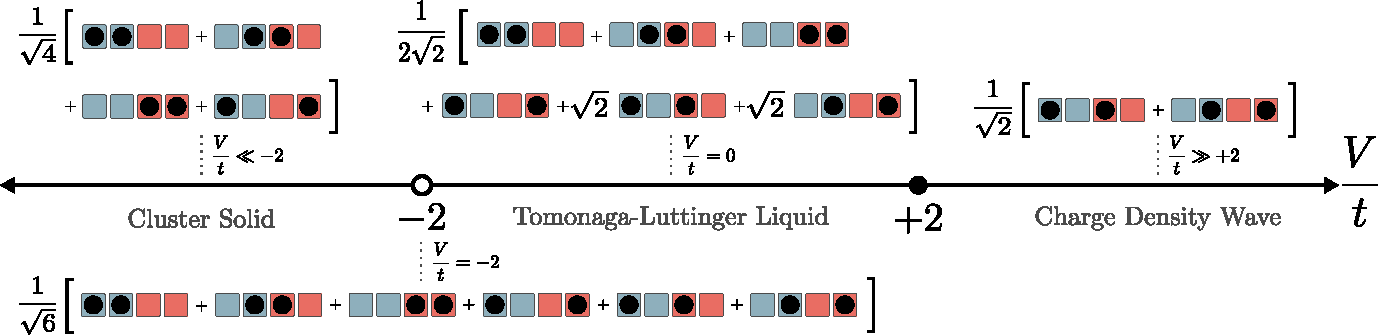
\includegraphics[width=1.0\textwidth]{phaseDiagramTV.pdf}
\end{center}
\caption{Phase diagram of the $t-V$ model accompanied by pictures of candidate ground states for $N=2$ fermions on a $L=4$ site lattice. For the purposes of measuring accessible entanglement, the lattice has been bipartitioned into spatial subregions $A$ (blue) and $B$ (red), each of size $\ell = 2$. We assume periodic boundary conditions. In the limit of strong attractive interactions where $V/t \ll -2$, the particles cluster together and there are $L$ equally probable configurations corresponding to all translations of the cluster.  At the first order phase transition where $V/t = -2$, all ${L}\choose{N}$ configurations are equally probable resulting in a flat state. In the TLL phase with $|V/t| < 2$,  particles are delocalized and we have included a characteristic state corresponding to free fermions $(V=0)$. In the limit of strong repulsive interactions where $V/t \gg 2$, fermions maximize their distance from each other resulting in a charge density wave (CDW) phase. The open and closed circles on the $V/t$ axis denote a first order and continuous phase transition, respectively.}
\label{fig:phaseDiagram}
\end{figure*}
%%%%%%%%%%%%%%%%%
\fi

\section{Numerical Results}


%In this section, numerical results obtained using exact diagonalization are shown. First, the finite size scaling of $S_{\alpha}^{\rm acc}(\rho_{A})$ will be illustrated. Following, the results correp

\subsection{Finite size scaling of the accessible entanglement}


%
%%%%%%%%%%
\begin{figure}[htp]
\begin{center}
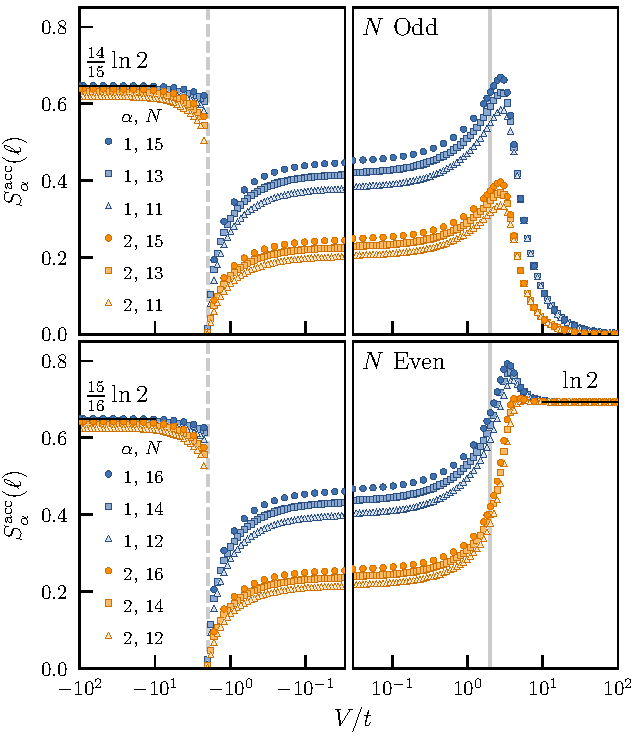
\includegraphics[width=1.0\columnwidth]{operationalEntanglementEntropies_SOP5.pdf}
\end{center}
\caption{Accessible entanglement entropy $S_{\alpha}^{\mathrm{acc}}(\ell)$ for $\alpha = 1, 2$ in the ground state of the $t-V$ model as a function of interaction strength $V/t$. The top panel shows the results for an odd number of total particles: $N=11,13,15$ and the bottom, for even: $N=12,14,16$. The gray vertical lines indicate the locations of the known phase transitions for the model, $V/t = \pm 2$. For $N=15,16$ the asymptotic results computed in Section~\ref{tab:Iimits} in the limits $V/t \to \pm \infty$ for $S_{1}^{\mathrm{acc}}$ are shown. \todo[inline]{EC: switch to a dashed line for the 1st order phase transition in all figures.}}
\label{fig:OEE}
 \end{figure}
%%%%%%%%%%

Figure \ref{fig:OEE} shows the accessible R\'enyi entanglement entropy values at interaction strengths in the interval $V/t: \left( -100,100 \right)$. This interval spans the three phases of the $tV$ model. For large negative interaction strengths, there is agreement between the values at which $S_{\alpha}^{\rm acc}(\rho_A)$ converges and the predicted value from \ref{tab:Limits} for all system sizes and $\alpha$. For large positive interaction strengths, the predicted effect of total particle number parity is observed. For $N$ odd, the accessible entanglement vanishes, whereas it converges to $\ln{2} \approx 0.6931 \dots$ for $N$ even, independent of system size and $\alpha$. At the first order phase transition $V/t=-2$, $S_{\alpha}^{\rm acc}(\rho_A)$, as expected. Thus, the asymptotic predictions for the accessible entanglement entropy in the $tV$ model have been confirmed via exact diagonalization. Increasing the magnitude of both the attractive and repulsive interactions will result in even more agreement between simulation and theory.

Recall that the accessible entanglement should be a monotonically decreasing function of $\alpha$. Figure $\ref{fig:OEE}$ supports this inverse relation since it is seen that $S_{1} \geq S_{2}$ $\forall$ $V/t \in \left( -100,100 \right)$.

Another interesting feature is the peak seen near the continuous phase transition $V/t=2$. Results seem to indicate that the peak is slightly shifting to the left, closer to $V/t=2$ as the number of particles $N$ increases. In an effort to find how the location of this peak scales with particle number, $V/t\vert_{Max}$ was obtained for various system sizes, where $V/t\vert_{Max}$ is the interaction strength at which the accessible entanglement peak occurs. Figure \ref{fig:peakScalingOddN} shows a plot of $V/t\vert_{Max}$ vs $N^{-0.3066}$. The exponent comes from a linear fitting of $\left( V/t\vert_{Max} - 2 \right)$ vs $N$ data. The observed inverse power law scaling is promising as all points fall on a line with $y$ intercept of $V/t\vert_{Max} = 2$, which is the exact value of the continuous phase transition in the asymptotic limit of $N \to \infty$ total particles.

%%%%%%%%%%
\begin{figure}[htp]
\begin{center}
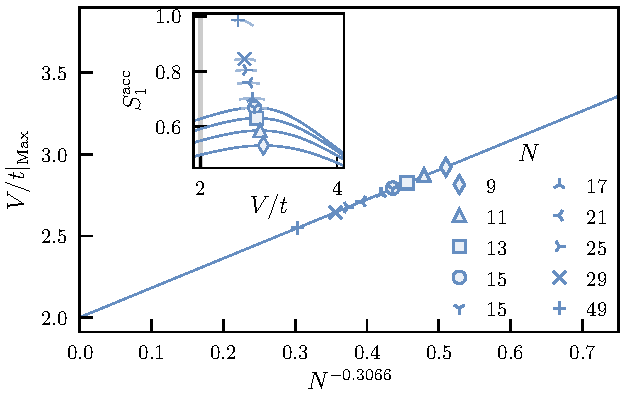
\includegraphics[width=1.0\columnwidth]{peakScalingOddN.pdf}
\end{center}
\caption{Interaction strength at which the maximum $S_{1}^{\mathrm{acc}}$ occurs as a function of the total number of particles $N$. The exponent of $N$ was obtained from a linear fitting of $\ln N$ vs. $\ln{(V/t - 2)}$.  Although very few points are plotted due to memory limitations, they agree with the hypothesis that for $N \to \infty$, the peak of Von Neumann accessible entanglement occurs at the phase transition $V/t = 2$. Inset: $S_{1}^{\mathrm{acc}}$ as a function of interaction strength $V/t$ for various $N$ around the neighborhood of the peak.}
\label{fig:peakScalingOddN}
\end{figure}
%%%%%%%%%%

\subsection{Entanglement of local particle number fluctuations}

Recall from section \ref{sec:accEntanglementIntro} that the difference between the full and the operationally accessible entanglement Von Neumann entropies $\left( \alpha = 1 \right)$ should equal the Shannon Entropy of the local particle number probability distribution $P_n$:

%
\begin{equation}
    \Delta S_1 (\rho_A) \equiv S_1(\rho_A) - S_1^{\rm acc}(\rho_A) = H_1(\{P_n\})
    \label{eq:DeltaS1}
\end{equation}
%

where

%
\begin{equation}
    H_1(\{P_n\}) = -\sum_{n=0}^N P_n \ln P_n.
\label{eq:H1}
\end{equation}

is the Shannon Entropy of the probability distribution of the local particle number $P_n$.

In this section, a comparison is done between the Shannon Entropy of the local particle number distribution and the difference between full and accessible entanglement. First, numerical results for this difference will be shown for the case of $\alpha=1$ and compared to the exact value of the Shannon Entropy of normally distributed local particle numbers. Then, higher values of $\alpha$ will be studied and the difference will be compared with the Shannon Entropy of the corresponding probability distribution of local particle number.

 %%%%%%%%%%
\begin{figure}[htp]
\begin{center}
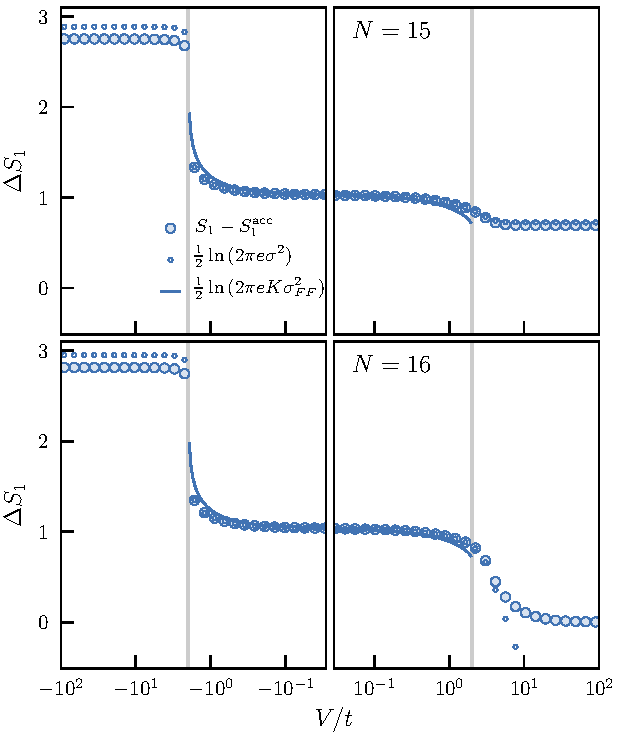
\includegraphics[width=1.0\columnwidth]{deltaS1_N15N16.pdf}
\end{center}
\caption{Difference between the von Neumann and accessible entanglement entropies $S_{1}-S_{1}^{acc}$ and $\frac{1}{2} \ln 2 \pi e \sigma^2$ as functions of interaction strength $V/t$. The latter expression is the well known differential entropy of a Gaussian distribution. In TLL phase ($-2 < V/t < 2$), the probability distribution is Gaussian, as can be seen from the agreement between the two results. The solid lines use the theoretical variance of particle number in $A$ inside the $LL$ phase, $K \sigma^2_{FF}$, where $K$ is the Luttinger parameter and is a function of $V/t$ and $\sigma^2_{FF}$ is the exact variance for free-fermions ($V/t = 0$).}
\label{fig:deltaS1}
\end{figure}
%%%%%%%%%%

%
Figure \ref{fig:deltaS1} shows the difference between the full and accessible Von Neumann entanglement entropies as a function of interaction strength. From exact diagonalization, the full ($S_1$), accessible ($S_{1}^{\rm acc}$) Von Neumann entanglement entropies and the variance of local particle number $n$ ($\sigma$) were obtained. Expecting that local particle number fluctuations are normally distributed in the TLL phase ($-2 < V/t < 2$) of the $tV$ model, these variances were inserted into the expression for the Shannon entropy of a Normal Distribution $\frac{1}{2}\ln{\left( 2\pi e \sigma^2 \right)}$. Additionally, the Shannon Entropy was calculated using the variance of local particle number predicted by Tomonaga-Luttinger Liquid theory $\sigma \equiv K\sigma_{FF}$ where $\sigma_{FF}$ is the variance of free-fermions $V/t = 0$ and $K$ is the Luttinger Parameter $K = \pi/(\cos^{-1}\left( -V/2t \right))$. The figure shows agreement between the three expressions in the TLL phase.


%%%%%%%%%%
\begin{figure}[htp]
\begin{center}
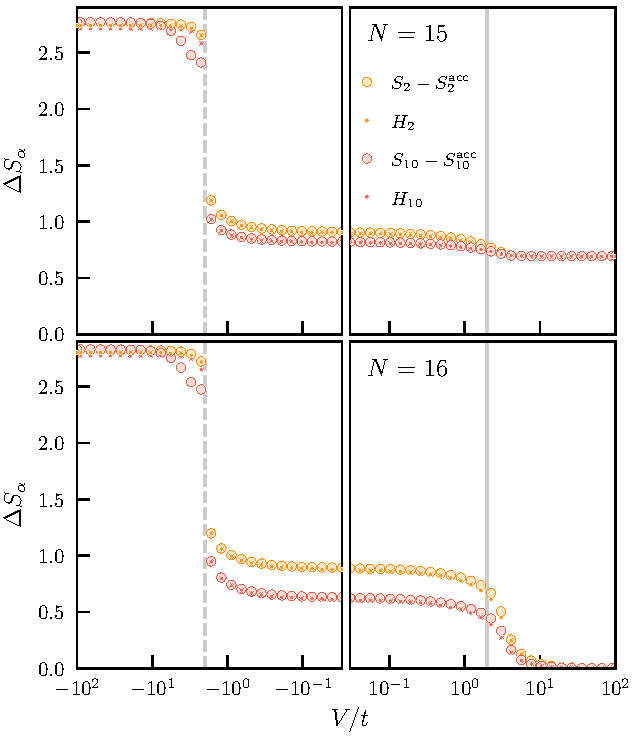
\includegraphics[width=1.0\columnwidth]{higherAlphaDeltaS_N15N16.pdf}
\end{center}
\caption{Difference between the \ren and accessible entanglement entropy $S_{\alpha} - S_{\alpha}^{\mathrm{acc}}$ and $H_{\alpha}$ as functions of interaction strength $V/t$ for $\alpha=2,10$. In general, $H_{\alpha}$ should provide a lower bound for $\Delta S_{\alpha}$ (i.e, $H_{\alpha} \leq S_{\alpha}$). Also, $S_{\alpha}^{\mathrm{acc}}$ should be non-increasing in $\alpha$. It can be seen that both relations hold in all phases of the $t-V$ model.}
\label{fig:deltaS_alpha}
\end{figure}
%%%%%%%%%%

At R\'enyi indices higher than $\alpha = 1$, the difference between the full and accessible entanglement entropies should be bounded from below by the classical R\'enyi entropy of the local particle number probability distribution $H_{\alpha}\left(\{P_n\}\right) = \ln{ \sum_{n} P_{n}^{\alpha}}/(1-\alpha)$. Figure \ref{fig:deltaS_alpha} shows $\Delta S_{\alpha}$ and $H_{\alpha}\left(\{P_n\}\right)$ as a function of interaction strength for R\'enyi indices $\alpha=2$ and $\alpha=10$. Not only in all cases is $H_{\alpha}\left(\{P_n\}\right) \leq \Delta S_{\alpha}$, but also the values corresponding to $\alpha=10$ are lower than the ones corresponding to $\alpha=2$, satisfying the condition that the difference in full and accessible entanglement should be a monotonically decreasing function of $\alpha$. The fact there's such good agreement for the $\alpha=2$ and $\alpha=10$ is rather astounding. Taking a look at Figure $\ref{fig:Halpha}$ reveals that the difference between the computationally determined R\'enyi entropy of $P_n$ and the theoretical value is proportional to the R\'enyi index. For $\alpha=10$, this difference is large enough that the agreement in the TLL phase in Figure \ref{fig:deltaS_alpha} is surprising. Up next, it will be shown that this agreement is a result of the proportionality between $P_{n,\alpha}$ and $P_n^{\alpha}$.

%%%%%%%%%%
\begin{figure}[htp]
\begin{center}
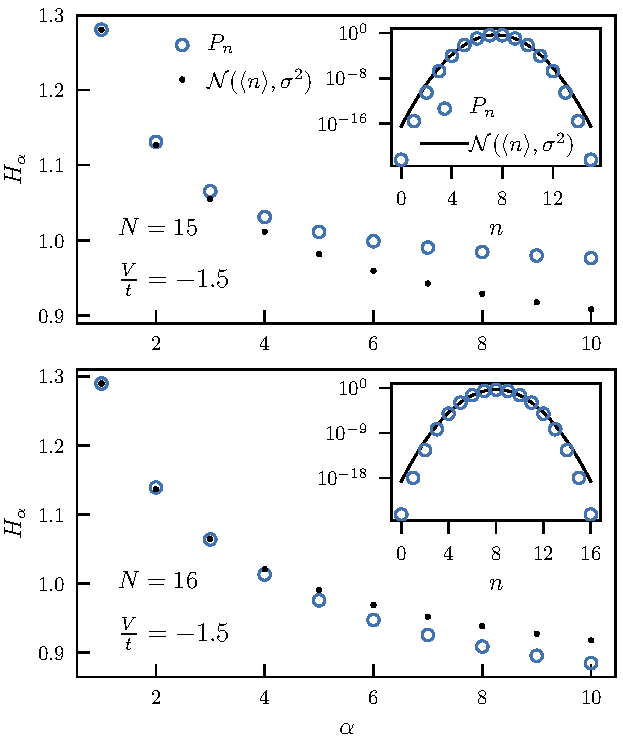
\includegraphics[width=1.0\columnwidth]{Halpha.pdf}
\end{center}
\caption{For $N=15$, $\sigma^2=0.758$ and for $N=16$, $\sigma^2=0.772$.}
\label{fig:Halpha}
 \end{figure}
%%%%%%%%%%

Recall the distribution defined in section \ref{sec:accEntanglementIntro}:
%
\begin{equation}
P_{n,\alpha} = \frac{P_{n}}{\Tr\rho_{A}^{\alpha}}
\label{eq:Pna}
\end{equation}
 %
 
which due to a normal distribution of local particle numbers  in the TLL phase of the $tV$ model ($-2 < V/t < 2$) can be approximated as:
%
\begin{equation}
P_{n,\alpha} \approx \sqrt{\frac{\pi\alpha}{2K\ln{\ell}}} e^{\frac{-\alpha \pi^2 (n - \langle n \rangle^2 )}{2K\ln{\ell}}} 
\label{eq:Pna_TLL}
\end{equation}
 %
 
Notice that raising Eq. \ref{eq:Pna_TLL} to either $1/\alpha$ or $K$ on both sides should get rid of the $\alpha$ or $K$ dependence of the exponential factor, respectively, within the TLL regime. The square root factor will still pick up the dependence on either of the exponents. In other words, raising by $1/\alpha$ or $K$ should give:
 
 \begin{equation}
 P_{n,\alpha}^{1/\alpha} \approx \sqrt{\frac{\pi\alpha}{2K\ln{\ell}}}^{1/\alpha} e^{\frac{- \pi^2 (n - \langle n \rangle^2 )}{2K\ln{\ell}}} 
 \label{eq:Pna_to_alphaInv}
 \end{equation}
 
 and
 
 \begin{equation}
 P_{n,\alpha}^{K} \approx \sqrt{\frac{\pi\alpha}{2K\ln{\ell}}}^K e^{\frac{- \alpha \pi^2 (n - \langle n \rangle^2 )}{2\ln{\ell}}} 
 \label{eq:Pna_to_K}
 \end{equation}
 
 %%%%%%%%%%
\begin{figure}[htp]
\begin{center}
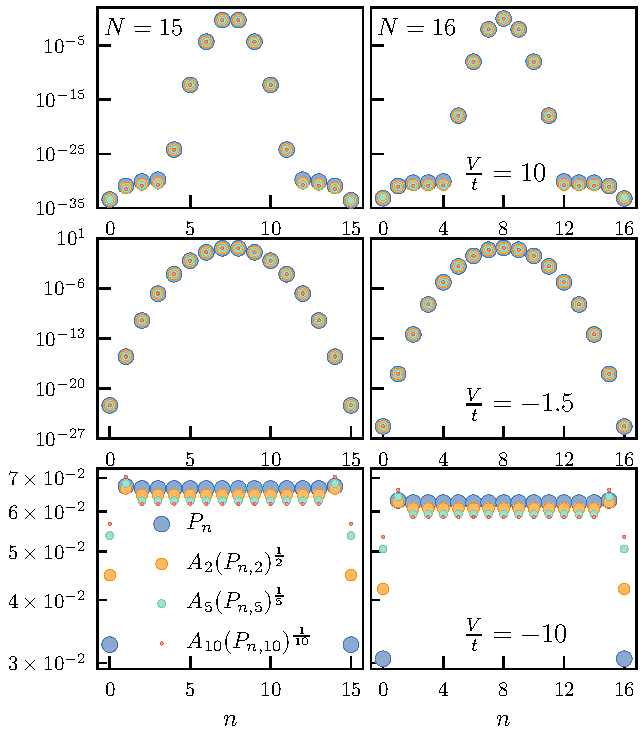
\includegraphics[width=1.0\columnwidth]{alphaCollapse.pdf}
\end{center}
\caption{Probabilities of measuring a state with $n$ particles in subregion $A$, as  a function of $n$. The probabilities in the $TLL$ regime are known to be Gaussian, as seen from Eq.6. Here, they have been raised to $1/\alpha$ in order to cancel out the $\alpha$ dependence of the exponential part. For the middle plot, the interaction strength lies in the $TLL$ regime and, consequently, the probabilities collapse to the same values in all the range after the $\alpha$ dependence has been cancelled. The top and bottom plots show results outside of the $TLL$ regime, where the probabilities are not Gaussian.}
\label{fig:alpha_collapse}
\end{figure}
%%%%%%%%%%
 
 Figure \ref{fig:alpha_collapse} shows the distribution $A_{\alpha} P_{n,\alpha}^{1/\alpha}$ for various interaction strengths $V/t$ and, thus, $K$. The constant $A_{\alpha}$ is the inverse of the square root factor in Eq. \ref{eq:Pna_to_alphaInv}. Cancelling the square root factor allows for a direct comparison of the exponential factor for each of the $\alpha$ values used. The middle plots confirm that this exponential factor indeed is independent of $\alpha$, illustrated by the fact that the distributions become the same for $\alpha=\{1,2,5,10\}$, when inside the TLL regime of $-2 < V/t < 2$.
 
%%%%%%%%%%
\begin{figure}[htp]
\begin{center}
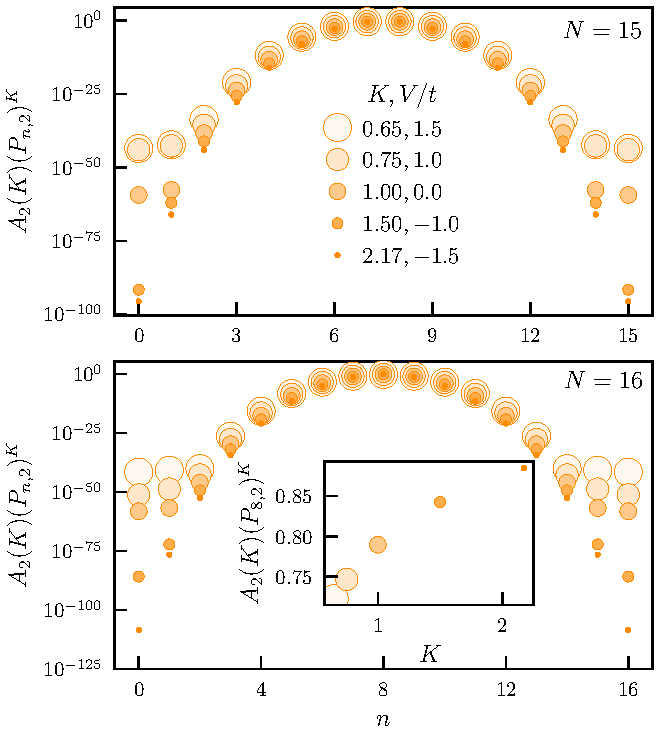
\includegraphics[width=1.0\columnwidth]{TLLCollapse.pdf}
\end{center}
\caption{Probabilities of measuring a state with $n$ particles in subregion $A$, as  a function of $n$. This time, the probabilities have been raised to the Luttinger Parameter $K$, after calculating for several $K$ values. The probabilities seem to collapse nearly to the same value near the middle of the distribution. The inset plot shows the $K$ dependence of the probability for fixed particle number in $A$, $n=8$. This helps illustrate that the probabilities are proportional to $K$ near the middle, as opposed to inversely proportional at the ends.}
\label{fig:K_collapse}
\end{figure}
%%%%%%%%%%
 
Figure \ref{fig:K_collapse} shows the distribution $A_{\alpha} P_{n,\alpha}^{K}$ with the R\'enyi index fixed at $\alpha=2$ and at various interaction strengths $V/t$ and corresponding Luttinger parameters $K$. In this case, the factor $A_{\alpha}$ is the inverse of the square root factor in Eq. \ref{eq:Pna_to_K}. All of the interaction strengths fall within the TLL regime and as such, all the distributions should become the same for the various $V/t$ and, thus, $K$ values. This collapse of the distributions at various $K$ is evident from looking at regions near the middle of the graph. Although it may not be apparent at first glance due to the scale, the tails of the distribution are all essentially zero.

\section{Conclusion}
In this chapter, the operationally accessible R\'enyi entanglement entropy was introduced in both it's original and generalized form. Analytical values of the entanglement entropy were obtained at various special cases of the $tV$ model and then confirmed via exact diagonalization. A maximum value in accessible entanglement was observed and evidence seems to support that it follows an inverse power law scaling in total particle number with scaling exponent of $-0.3066$. 

The difference in full and accessible entanglement entropies was also computationally determined and it was confirmed that in the TLL phase of the $tV$ model, it is equal to the the R\'enyi entropy of a Normal Distribution of local particle number. Finally, it was then proposed theoretically and confirmed computationally, that getting rid of its R\'enyi index and Luttinger parameter dependence, the exponential part of these Normal Distributions depend exclusively on local particle number fluctuations.

\iffalse
%Figure 8
%%%%%%%%%%
\begin{figure}[htp]
\begin{center}
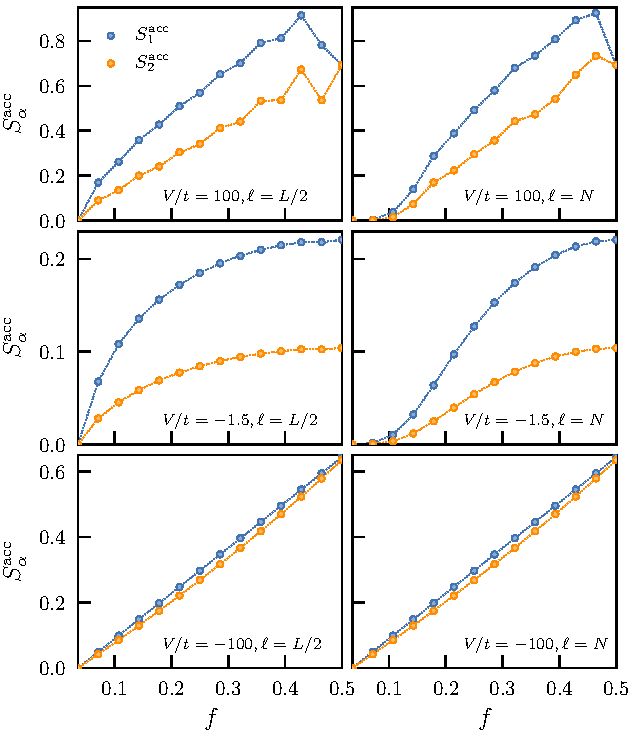
\includegraphics[width=1.0\columnwidth]{fillingFractionDependence.pdf}
\end{center}
\caption{Accessible entanglement entropies $S_{\alpha}^{\mathrm{acc}}(\ell)$ for $\alpha = 1,2$ as a function of filling fraction $N/L$. The lattice size was kept fixed at $L=28$ sites and the total number of particles were $N=1,2,3...14$. For the left column, the spatial partition $\ell$ was kept fixed at half the lattice size, $\ell = L/2$. For the right column, it was set to equal the total number of particles $N$. The interaction strengths $V/t$ are indicated in each of the plots and correspond to values from each of the three phases of the $t-V$ model.}
\label{fig:fillingFractionDependence}
\end{figure}
%%%%%%%%%%
\fi




\chapter{Conclusions and Future Work}
\section{Chapter 4}

	In this chapter, future projects are discussed. Some of these projects stem from unanswered questions in previous work, while some of them will be completely new.
	
	\subsection{Power law scaling of entanglement peak in the $tV$ model}
	
	%%%%%%%%%%
	\begin{figure}[h]
	\begin{center}
	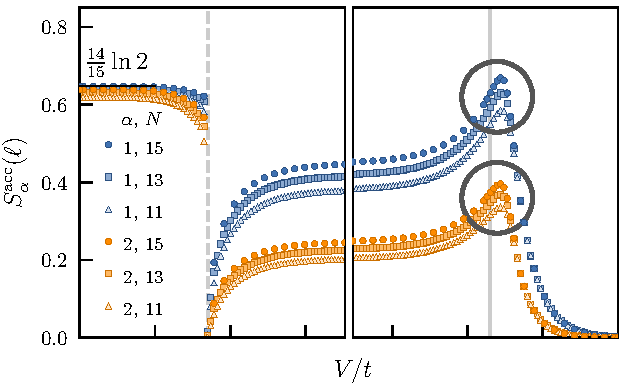
\includegraphics[scale=1.0]{operationalEntanglementEntropies_SOP5_withPeakCircles.pdf}
	\end{center}
	\caption{Accessible entanglement entropies as a function of interaction strength in the $t-V$ model. The circles enclose a region where both the von Neumann and R\'enyi entanglement entropies attain a maximum value. As the total number of particles $N$ increases, this maximum seems to be shifting to the left, closer to the phase transition $V/t=2$.}
	\label{fig:OEE_circledPeaks}
	\end{figure}
	%%%%%%%%%%
	
	In the $t-V$ model, there are two known phase transitions, a first order one at $V/t=-2$, and a continuous one at $V/t=2$. From Figure \ref{fig:OEE_circledPeaks}, it can be seen that the accessible entanglement entropies are sensitive to both types of transition. Interestingly, this sensitivity to the transition in $V/t=2$ expresses itself as a peak of entanglement. Moreover, the interaction strength at which this peak of entanglement occurs moves closer to the exact value of the continuous phase transition as the number of particles in the system increases.  
	
	%%%%%%%%%%
	\begin{figure}[h!]
	\begin{center}
	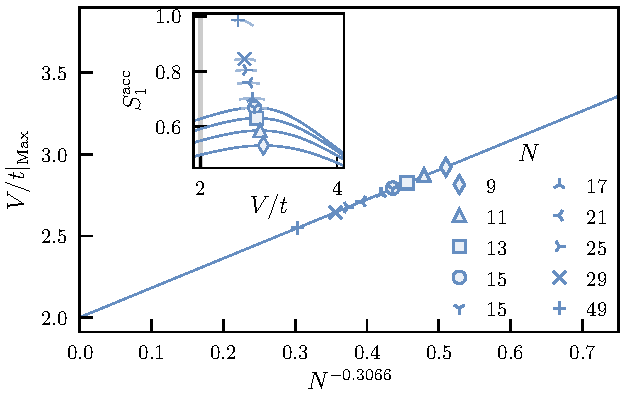
\includegraphics[scale=1.0]{peakScalingOddN.pdf}
	\end{center}
	\caption{Interaction strength at which the maximum $S_{1}^{\mathrm{acc}}$ occurs as a 	function of the total number of particles $N$. The exponent of $N$ was obtained from a l	inear fitting of $\ln N$ vs. $\ln{(V/t - 2)}$.  Although very few points are plotted due to 	memory limitations, they agree with the hypothesis that for $N \to \infty$, the peak of 	von Neumann accessible entanglement occurs at the phase transition $V/t = 2$. Inset: 	$S_{1}^{\mathrm{acc}}$ as a function of interaction strength $V/t$ for various $N$ 		around the neighborhood of the peak.}
	\label{fig:peakScalingOddN}
	\end{figure}
	%%%%%%%%%%
	
	Figure \ref{fig:peakScalingOddN} shows the value where the entanglement peak occurs for various system sizes. The fact that all the points lie on a line that intercepts the vertical axis at $V/t_{Max}=2$ is very promising. Nevertheless, the current scaling exponent of $-0.2545$ should not be taken for granted due to how small the systems currently are. Indeed, the continuous phase transition should occur in the $t-V$ model at $V/t=2$, but this is for a system where $N \to \infty$. More data points, corresponding to large systems are still be needed to get closer to this intercept and confirm the power law scaling.	

	
	\subsection{Filling fraction dependence of entanglement}
	
	The $t-V$ model results presented in this thesis were focused on the special case of half filling. That is, only half of the lattice sites were had particles in them ($N = L/2$). For this case, the exact results for the phase transitions are mapped from the XXZ spin-$1/2$ model. For other filling fraction, a theory has yet to be developed. Figure \ref{fig:fillingFractionDependence} shows the accessible entanglement entropies for various filling fractions ranging from $1/14$ to $1/2$. 
	
	%Figure 8
	%%%%%%%%%%
	\begin{figure}[h!]
	\begin{center}
	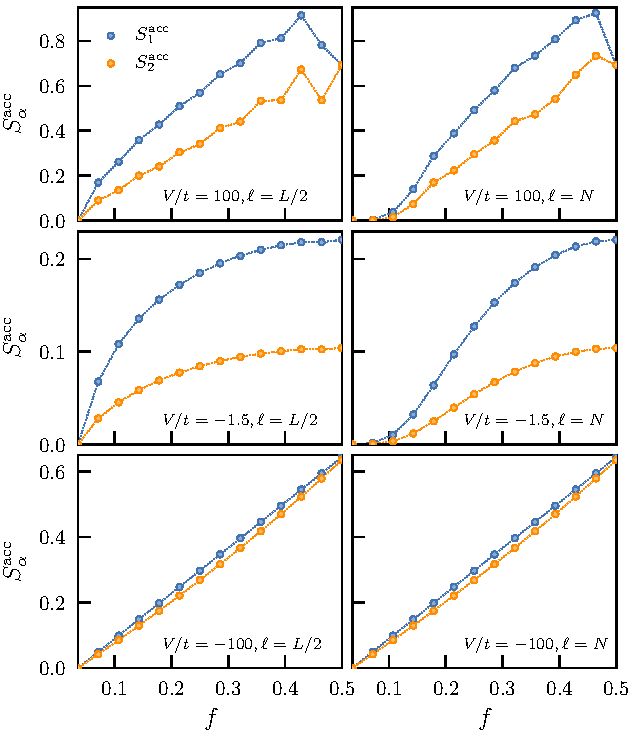
\includegraphics[scale=1.0]{fillingFractionDependence.pdf}
	\end{center}
	\caption{Accessible entanglement entropies $S_{\alpha}^{\mathrm{acc}}(\ell)$ for $		\alpha = 1,2$ as a function of filling fraction $N/L$. The lattice size was kept fixed at 		$L=28$ sites and the total number of particles were $N=1,2,3...14$. For the left column, 	the spatial partition $\ell$ was kept fixed at half the lattice size, $\ell = L/2$. For the right 	column, it was set to equal the total number of particles $N$. The interaction strengths 	$V/t$ are indicated in each of the plots and correspond to values from each of the three 	phases of the $t-V$ model.}
	\label{fig:fillingFractionDependence}
	\end{figure}
	%%%%%%%%%%
	
	\subsection{Accessible entanglement via quantum gates}
	
	The endgame for the study of accessible entanglement entropies is to exploit the entanglement of a system as a resource. Motivated by this, we are currently working on building a quantum circuit that reproduces the accessible entanglement measurement process. After coming up with the appropriate quantum circuit, the results will be tested on IBM's quantum computer \cite{IBMQuantumExp:2018:Online}.
	
	\subsection{Entanglement in the Bose-Hubbard model}
	
	Another project in the works is calculating accessible entanglement entropies in the Bose-Hubbard (BH) model. In the study of fermionic systems, such as the $t-V$ model, methods like exact diagonalization and density matrix renormalization group must be used to due to the infamous sign problem. The high memory cost of these methods restricts simulations to only relatively small system sizes. Nevertheless, the sign problem non-existent in bosonic models and thus quantum Monte Carlo (QMC) methods can be used. QMC will allow the study of much larger systems than the ones presented here.

\addcontentsline{toc}{chapter}{Appendices}
\appendix

\chapter{}
%\section{Site to momentum basis mapping of kinetic operator}
\label{appendix:kineticMapping}

The kinetic energy operator of the fermionic $t-V$ Model is:

\[\hat{T} = -t \sum_{i} c_{i}^{\dagger} c_{i+1} + h.c\]

where $t$ is the hopping amplitude, $c_{i}$ ($c_{i}^{\dagger}$) is the fermionic annihilation (creation) operator on site $i$, $h.c$ stands for "Hermitian Conjugate" and the sum is carried over all lattice sites. This operator describes a fermion hopping between neighboring sites. Nevertheless, it may not be obvious in a physical sense how this expression 'counts' the contribution to the kinetic energy in the model. Here it will be shown that:

\[-t \sum_{i} c_{i}^{\dagger} c_{i+1} + h.c = \sum_{k} \epsilon(k) n_{k} \]

where $\epsilon(k)$ is the dispersion relation of a fermion with momentum $p_{k} = \hbar k$ and $n_{k}$ counts how many fermions have wavenumber $k$. Hopefully, the expression on the right makes conceptually clearer how the kinetic energy operator is actually counting the total kinetic energy of a state. To move from real space to $k-space$, the discrete version of the Fourier Transform will be applied to the fermionic creation and annihilation operators. 

Consider a lattice with $L$ total sites. The Discrete Fourier Transform (DFT) is defined as:

\[ f_{j} = \frac{1}{\sqrt{L}} \sum_{k} f_{k} e^{ikj} \]

The index $j$ has been chosen to represent the lattice sites in order to avoid confusion with the imaginary unit, $i$.

Thus, applying the DFT to the creation and annihilation operators:

\[ c_{j}^{\dagger} = \frac{1}{\sqrt{L}} \sum_{k} e^{-ikj} c_{k}^{\dagger} \] 
\[c_{j} = \frac{1}{\sqrt{L}} \sum_{k} e^{ikj} c_{k}\]

Now, consider the first term of the kinetic operator (without the $-t$, for now) and substitute these 'transformed' operators:

\[ \begin{aligned}
\sum_{j} c_{j}^{\dagger} c_{j+1} &= \sum_{j} [\frac{1}{\sqrt{L}} \sum_{k} e^{-ikj} c_{k}^{\dagger} \frac{1}{\sqrt{L}} \sum_{k'} e^{ik'(j+1)} c_{k'} ] \\
&= \frac{1}{L} \sum_{j} [\sum_{k} \sum_{k'}  c_{k}^{\dagger} c_{k'} e^{i(k'-k)j} e^{ik'}] \\
&= \sum_{k} \sum_{k'}  c_{k}^{\dagger} c_{k'} e^{ik'} \underbrace{\frac{1}{L} \sum_{j} e^{i(k'-k)j}}_{\stackrel{def}{=} \delta_{kk'}} \\
&= \sum_{k} \sum_{k'}  c_{k}^{\dagger} c_{k'} e^{ik'} \delta_{kk'} ; \text{ only the k'=k term 'survives'} \\
\sum_{j} c_{j}^{\dagger} c_{j+1} &= \sum_{k} c_{k}^{\dagger} c_{k} e^{ik} \\
\end{aligned} \]

The Hermitian Conjugate of this gives the second term in the operator. It is obtained almost for free from the above result:

\[ \sum_{j} c_{j+1}^{\dagger} c_{j} = \sum_{k} c_{k}^{\dagger} c_{k} e^{-ik} \]

Adding the last two lines and multiplying by (minus) the hopping amplitude $t$:

\[ \begin {aligned}
-t \sum_{j} [ c_{j}^{\dagger} c_{j+1} + c_{j+1}^{\dagger} c_{j} ] &= -t \sum_{k} [c_{k}^{\dagger} c_{k} e^{ik} + c_{k}^{\dagger} c_{k} e^{-ik}] \\
&= -t \sum_{k} [c_{k}^{\dagger} c_{k} (e^{ik} + e^{-ik})] \\
&= -t \sum_{k} [c_{k}^{\dagger} c_{k} (2\cos(k))] \\
&= \sum_{k} [\underbrace{c_{k}^{\dagger} c_{k}}_{n_{k}} \underbrace{(-2t\cos(k))}_{\epsilon(k)}] \\
\end {aligned} \]

Therefore:

\[ \hat{T} = -t \sum_{j} [ c_{j}^{\dagger} c_{j+1} + c_{j+1}^{\dagger} c_{j} ]  = \sum_{k} \epsilon(k) n_{k} \] Q.E.D

On a side note, the dispersion relation for fermions on a one dimensional lattice with lattice constant $a$ is: $\epsilon(k) = -2t\cos(ka)$, which was retrieved here for $a=1$.


\chapter{}
\section{Lanczos Algorithm}
\label{app:lanczos}

\subsection{Introduction}

The Lanczos Algorithm, takes as input a Hermitian Matrix and iteratively builds a similarity transform that makes it tridiagonal. Due to similarity, the solution of the eigenvalue problem of the tridiagonal matrix is the same as that of the original matrix. Nevertheless, some methods can exploit the tridiagonality to find the eigendecomposition more easily. In condensed matter physics, the input matrix is usually a Hamiltonian. The eigenvalues and eigenvectors of the Hamiltonian represent the energies and the associated quantum states of the system. 

In the following section, the Lanczos Algorithm will be derived. Next, some methods for approximating the eigenvalues and eigenvectors will be discussed. Finally, a hopefully simple implementation of the algorithm in Python will be linked and some results will be shown.

\subsection{Tridiagonalization of the original matrix}

Let $A$ be a Hermitian matrix of size $nxn$. An orthonormal transform matrix $Q$ is needed such that:
%
\begin{equation}
T = Q^{T}AQ 
\end{equation}
%
where $T$ is a tridiagonal and Hermitian matrix similar to A.

The idea is to obtain a recursive relation, starting from the known fact that $T$ is tridiagonal and that the columns of the transform $Q$ are mutually orthonormal. The matrix $T$ has the form:
%
\begin{equation}
T = \begin{pmatrix}
    \alpha_1 & \beta_1    &                &               &                         &                      & 0              \\
    \beta_1  & \alpha_2  & \beta_2   &               &                         &                      &                  \\
                 & \beta_2    & \alpha_3  & \beta_3  &                        &                      &                   \\
                 &                &  \beta_3    &\ddots    & \ddots             &                      &                    \\
                 &                 &           &     \ddots     &  \alpha_{n-2}   &  \beta_{n-2} &                     \\
                 &                 &           &                     & \beta_{n-2}     & \alpha_{n-1} & \beta_{n-1}  \\
             0  &                 &           &                     &                         & \beta_{n-1}   & \alpha_n      \\
 
  \end{pmatrix}
\end{equation}
%
Operating $Q$ on both sides of the similarity relation above from the left: 
%
\begin{equation}
QT = QQ^{T}AQ = IAQ= AQ
\end{equation}
%
Let $\lbrace q_1, q_2, q_3, ... , q_k \rbrace $ be represent the mutually orthonormal columns of $Q$ and $\lbrace t_1,t_2,t_3,...,t_k \rbrace$, those of $T$.  Then, at the $k$-th step of the Lanczos iteration:
%
\begin{align}
A q_k &= Q t_k \\
&= \begin{pmatrix} 
\dots & q_{1,k-1} & q_{1,k} & q_{1,k+1} & \dots \\
\dots & q_{2,k-1} & q_{2,k} & q_{2,k+1} & \dots \\
& & \vdots & & \\
\dots & q_{n,k-1} & q_{n,k} & q_{n,k+1} & \dots \\
\end{pmatrix} 
\begin{pmatrix}
\vdots \\
0 \\
\beta_{k-1}\\
\alpha_{k}\\
\beta_{k}\\
0 \\
\vdots \\
\end{pmatrix}
\end{align}
%
The column vector only has three nonzero components. Namely, $\beta_{k-1}$, $\alpha_{k}$ and $\beta_{k}$. Thus, the product of this matrix-vector multiplication becomes:
%
 \begin{align}
A q_k &= \begin{pmatrix}
q_{1,k-1} \\
q_{2,k-1} \\
\vdots \\
q_{n,k-1} \\
\end{pmatrix} \beta_{k-1} + 
\begin{pmatrix}
q_{1,k} \\
q_{2,k} \\
\vdots \\
q_{n,k} \\
\end{pmatrix} \alpha_{k} +
\begin{pmatrix}
q_{1,k+1} \\
q_{2,k+1} \\
\vdots \\
q_{n,k+1} \\
\end{pmatrix} \beta_{k} \\
\end{align}
%
Or, more compactly:
%
\begin{equation}
A q_{k} = \beta_{k-1} q_{k-1} + \alpha_{k} q_{k} + \beta_{k} q_{k+1}
\end{equation}
%
From this three-term recursion relation, $Q$ can be built by finding equations for the nonzero elements of the set of columns $\lbrace q_i \rbrace_{i=1}^{n}$ (i.e the $\alpha$'s and $\beta$'s). First, the $\alpha_k$ equation will be derived. Multiplying both sides of the three-term recursion relation by $q_{k}^{T}$ from the left:
%
\begin{equation} 
q_{k}^{T} A q_{k} = \beta_{k-1} q_{k}^{T}q_{k-1} + \alpha_{k} q_{k}^{T} q_{k} + \beta_{k} q_{k}^{T} q_{k+1}
\end{equation}
%
Since the columns of $Q$ are mutually orthonormal, $q_{k}^{T}q_{k'} = \delta_{kk'}$. In other words, the first and third term will vanish and the second one survives. The equation for $\alpha_{k}$ is then:
%
\begin{equation} 
\alpha_{k} = q_{k}^{T} A q_{k}
\end{equation}
%
To obtain the $\beta_{k}$ equation, first the recursion relation is solved for $\beta_{k}q_{k+1}$, which gives:
%
\begin{equation}
\beta_{k} q_{k+1} = A q_{k} - \alpha_k q_k + \beta_{k-1} q_{k-1} = (A-\alpha_k I) q_k - \beta_{k-1} q_{k-1}
\end{equation}
%

Setting $r_k \equiv (A-\alpha_k I) q_k - \beta_{k-1} q_{k-1}$:
%
\begin{equation}
\beta_{k} q_{k+1} = r_{k}
\end{equation}
%
Or
%
 \begin{equation}
q_{k+1} = \frac{r_k}{\beta_{k}}
\end{equation}
%
where $\beta_{k} \neq 0$ and, since $q_{k+1}$ is an orthonormal vector, $\beta_{k} = || r_k ||_2$, such that $q_{k+1}$ is normalized.

Note that the $\alpha_k$ and $\beta_k$ terms of the three-term recursion relation have been accounted for. As for the $\beta_{k-1}$, a "bottom rung" for the recursion has to be set. The tridiagonal matrix $T$ does not have a $\beta_{k-1}$ term. Thus, for $k=1$, the $\beta_{k-1} q_{k-1}$ term is set to $\beta_{0} q_{0} = 0$. Now the columns of $Q$ can be built by iterating from $k=1$ to $k=n$.

\subsection{Algorithm}

 1. Set $r_0=q_1$,$\beta_0=1$ and $q_0 = 0$ \\
  2. For k=1,2,3,...,n: \\
  3.     $q_{k+1} = \frac{r_k}{\beta_{k}}$ \\
  4.     $\alpha_k = q_k^T A q_k$ \\
  5.     $r_k = (A - \alpha_k I)q_k - \beta_{k-1}q_{k-1}$ \\
  6.     $\beta_k = ||r_k||_2$ \\
  7.     Reorthonormalize $\lbrace q_i \rbrace_{i=1}^{k}$ if necessary \\
  8.     Approximate Eigenvalues and Eigenvectors (Can be done after the loop instead) \\

Line $1$: $\beta_0$ is set to 1 since it is the norm of $r_0$ and $r_0 = q_1$, where $q_1$ is a normalized vector. \\

Line $2$: The for loop runs from $k=1$ all the way up to $k=n$, where $n$ is the total number of columns. Depending of the eigenvalues desired, this loop can instead be a while loop that ends whenever the eigenvalues have reached a desired tolerance. \\

Line $7$: Due to finite precision errors, the set of supposedly mutually orthonormal vectors $\lbrace q_i \rbrace_{i=1}^{k}$ will actually lose their orthonormality at later Lanczos steps. When this happens, a reorthonormalization scheme, such as the Grahm-Schmidt Process, has to be employed. \\

Line $8$: Again, depending on the problem and the desired eigenpairs, the approximation can be done for the current version of the tridiagonal matrix at step $k$, call it $T_k$. Alternatively, it could be done after the for loop has finished and the full tridiagonal matrix has been $T$ built. There is no strict requirement on which iterative method should be used to find the eigendecomposition (QR Method, Power Iteration, Inverse Power Iteration, etc...). 

\subsection{Code}

An implementation of the Lanczos Algorithm in Python can be found in: https://github.com/ecasiano/LanczosEigensolvers/blob/master/lanczosEigensolver.py. The code generates a random, sparse, hermitian matrix of specified size, finds a tridiagonal representation via Lanczos and calculates the full eigendecomposition via QR Algorithm or finds the smallest eigenvalue via Inverse Power Iteration. A blackbox function, part of the numpy.linalg package, numpy.linalg.eigsh(), solves the eigenvalue problem for the input matrix so a comparison can be made with the code results.

\subsection{Results}

The following colormap represents a sparse and hermitian matrix of dimensions $n x n$ that was fed to the linked Lanczos code. 

\begin{figure}[h]
\begin{center}
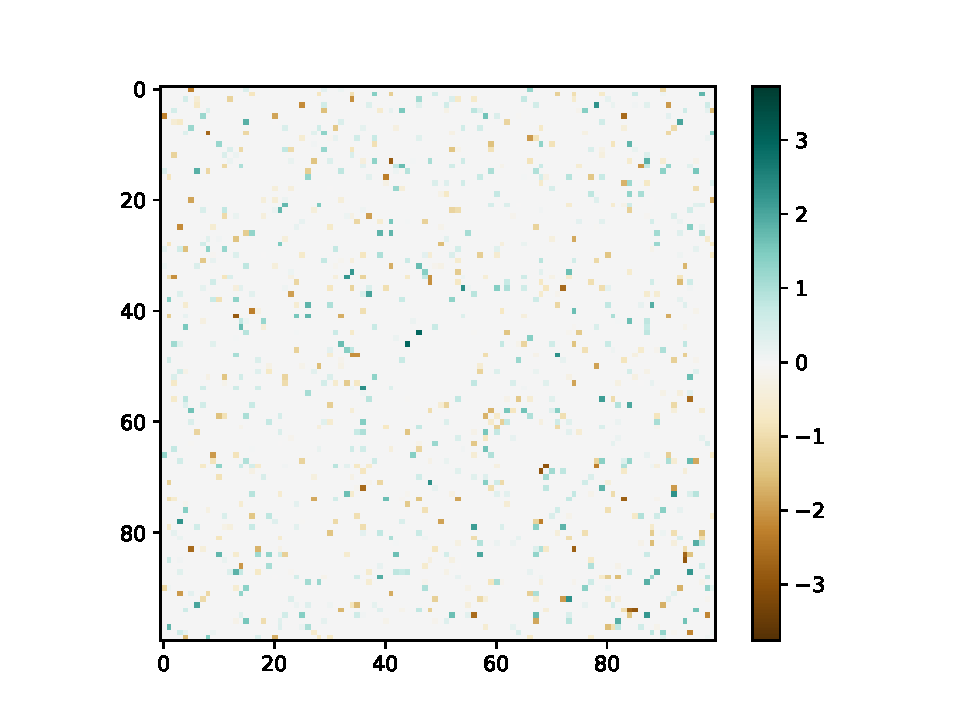
\includegraphics[width=0.7\columnwidth]{Images/Lanczos/A.pdf}
\end{center}
\caption{INSERT CAPTION.}
\label{fig:particle_partition}
\end{figure}

The Lanczos iterations were carried from $k=1$ to $k=n=100$. First, Lanczos was ran without reorthonormalizing the columns of the transform matrix $Q$.


\begin{figure}[h]
\begin{center}
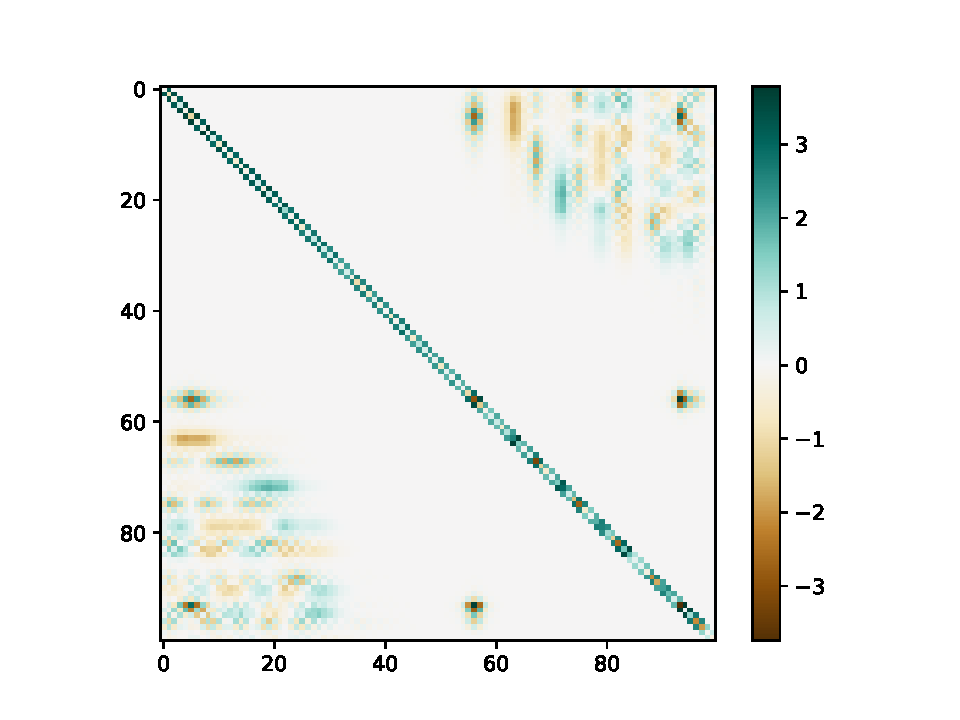
\includegraphics[width=0.7\columnwidth]{Images/Lanczos/T_noReortho.pdf}
\end{center}
\caption{INSERT CAPTION.}
\label{fig:particle_partition}
\end{figure}

Observe how the matrix starts to look tridiagonal, but has some large nonzero entries far away from the diagonal. This is the result of finite precision error. Via the Grahm-Schmidt Procedure, a full reorthonormalization was then done at each Lanczos step. The colormap below shows the result.

\begin{figure}[h]
\begin{center}
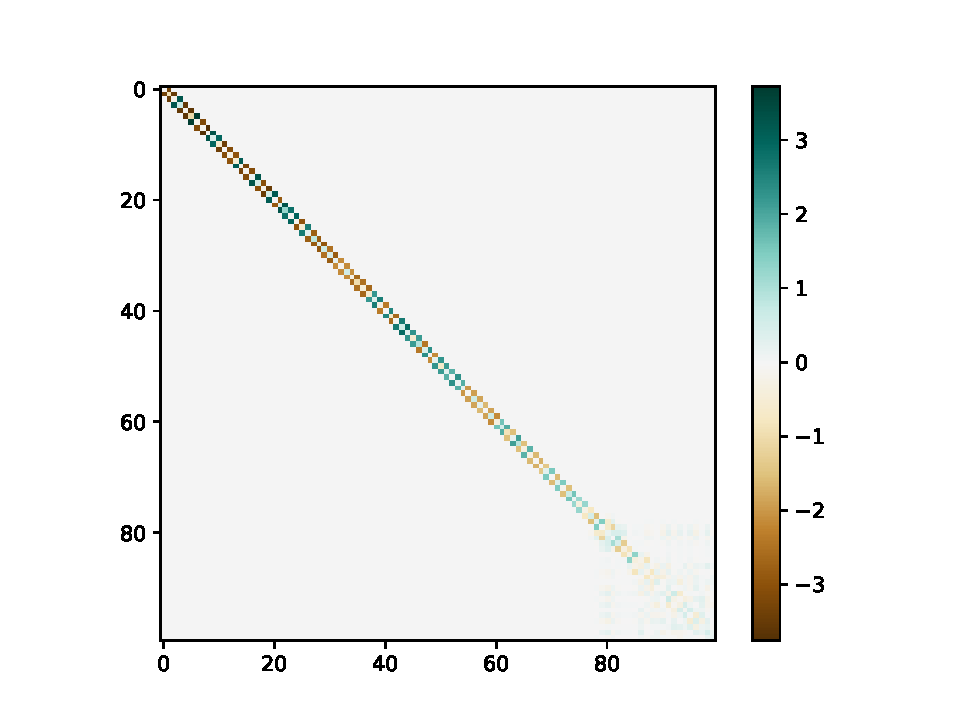
\includegraphics[width=0.7\columnwidth]{Images/Lanczos/T_yesReortho.pdf}
\end{center}
\caption{INSERT CAPTION.}
\label{fig:particle_partition}
\end{figure}

Barring some small nonzero entries in the bottom right, most likely due also to finite precision, the matrix was now tridiagonalized successfully.

The following scatter plot shows the eigenvalues obtained using the Lanczos code linked and those obtained using numpy.linalg.eigsh(). These eigenvalues correspond to the same matrix generated for the plots in the previous section.

\begin{figure}[h]
\begin{center}
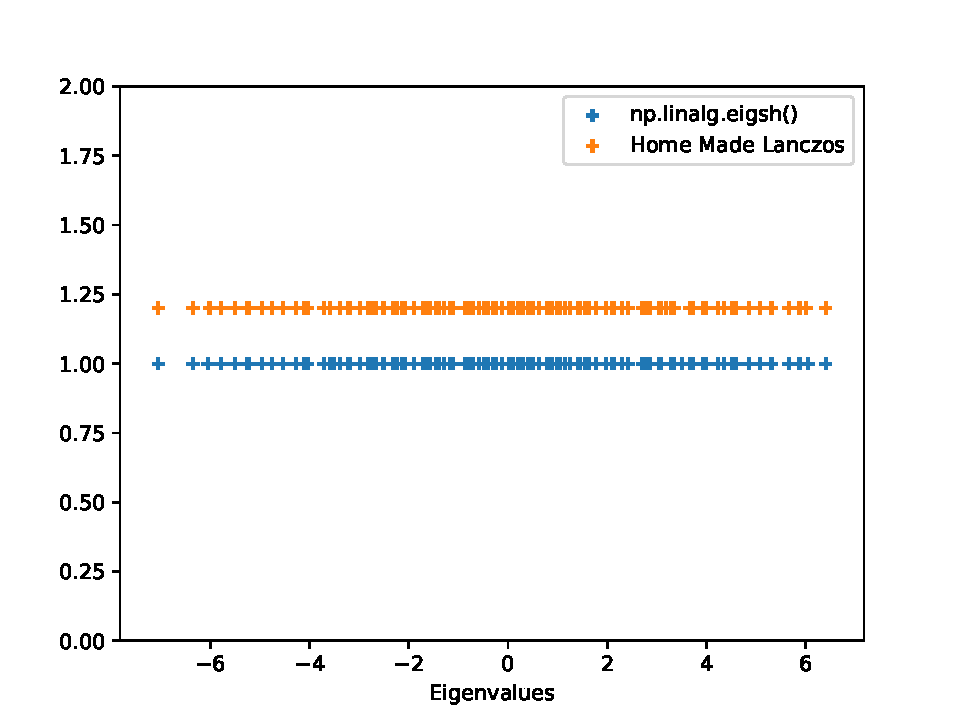
\includegraphics[width=0.7\columnwidth]{Images/Lanczos/eigenvaluesComparison.pdf}
\end{center}
\caption{INSERT CAPTION.}
\label{fig:particle_partition}
\end{figure}

\chapter{}
\label{appendix:appB}
\section{Evaluating the $n$-particle partition entanglement}

In this appendix, we show that the $n$-RDM of spinless hardcore particles on
a lattice can be written as a tensor product of two lower-rank matrices. This
simplification significantly reduces the numerical cost for calculating $n$-RDM
for such quantum systems. 

In general, for a pure quantum state $\vert \Psi\rangle$ in some
Hilbert space $\cal H$ that can be written as the tensor product space $A \otimes
B$, we can write

\begin{equation}
 \vert \Psi\rangle = \sum_{i,j} C_{i,j} \vert \psi^A_i\rangle  \vert \psi^B_j\rangle
\label{state_decomposition},
\end{equation}
where $\{\vert \psi^A_i\rangle\}$ and $\{\vert \psi^B_j\rangle\}$ are
orthonormal bases in the two Hilbert spaces $A$ and $B$, respectively.
Accordingly, the system degrees of freedom are bipartitioned between the two
subsets  $\{\vert \psi^A_i\rangle\}$ and $\{\vert \psi^B_j\rangle\}$. Using the
product basis $\{\vert \psi^A_i\rangle\vert  \psi^B_j\rangle\}$, the full
density matrix can be written as \begin{equation}
\rho=\vert \Psi\rangle\langle\Psi\vert = \sum_{i,j,i',j'}  \vert \psi^A_i\rangle  \vert \psi^B_j\rangle C_{i,j}C^*_{i',j'} \langle\psi^A_{i'}\vert \langle\psi^B_{j'}\vert 
\label{full_density_matrix}.
\end{equation}
The reduced density matrix $\rho_A$ ($\rho_B$) of subspace $A$ ($B$) , is obtained from $\rho$ by tracing out the degrees of freedom of subspace $B$ ($A$), 
\begin{equation}
\rho_A=\sum_{m}\langle\psi^B_m\vert \rho \vert \psi^B_m\rangle= \sum_{i,j}  \vert \psi^A_i\rangle \left(\sum_{m}C_{i,m}C^*_{j,m}\right) \langle\psi^A_{j}\vert 
\label{rho_1_full},
\end{equation}
\begin{equation}
\rho_B=\sum_{m}\langle\psi^A_m\vert \rho \vert \psi^A_m\rangle= \sum_{i,j}  \vert \psi^B_i\rangle \left(\sum_{m}C_{m,i}C^*_{m,j}\right) \langle\psi^B_{j}\vert 
\label{rho_2_full}.
\end{equation}
 Moreover,  the reduced density matrices can be generated using the linear maps $G_{AB}:S_B\rightarrow S_A$ as  $\rho_A=G_{AB}G_{AB}^\dagger$ and $\rho_B=(G_{AB}^\dagger G_{AB})^T$
where
\begin{equation}
G_{AB}=\sum_{i,j}C_{i,j}\vert \psi^A_i\rangle\langle\psi^B_j\vert 
\label{D_1}.
\end{equation}
Note that, in general, the matrix representing the linear maps $G_{AB}$ is
rectangular since the dimensions of the Hilbert spaces $A$ and $B$ can differ.

\subsection{Particle bipartition}
\label{sec:Particle_bipartition}
%(fermions, hardcore bosons or anyons)(Fock states)
Let us now consider a quantum system of $N$ spinless hardcore particles in a
state $\vert \Psi\rangle=\sum_i\chi_i \vert \psi^N_i\rangle$, where $\{\vert
\psi^N_i\rangle\}$ are the $N$ particle second-quantization basis states, where
each basis state corresponds to a single, possible, occupation number
configuration (ONC). Now we recall that each ONC state is a linear combination
of the distinguished particles states $\{\vert \psi^N_{i,j}\rangle\}$ as $\vert
\psi^N_i\rangle=\sum_j\frac{f_j}{\sqrt{N!}}\vert \psi^N_{i,j}\rangle$, where
$j$ runs over all  possible particle permutations (PPs) and $f_j=e^{-i\phi_j}$ is
the corresponding phase factor. Accordingly, we can write 
%
\begin{equation}
\vert \Psi\rangle=\sum_{i,j}\frac{\chi_if_j}{\sqrt{N!}}\vert \psi^N_{i,j}\rangle.
\label{Psi_pprho_1and2_star}
\end{equation}
%
%\subsection{Partitioning the particle}
%\label{subsec:Partitioning_the_particle}

Now we partition $N$ into two sets of particles: $n_A$ and the remainder 
$n_B=N-n_A$.  The distinguished particles basis $\{\vert \psi^N_{i,j}\rangle\}$
can be written as a tensor product of the two partitions basis 
%
\begin{equation}
\vert \psi^N_{i,j}\rangle=\vert \psi^{n_A}_{i_A,j_A}\rangle\vert \psi^{n_B}_{i_B,j_B}\rangle
\label{psiN_psin1n2},
\end{equation}
%
where each ONC (labelled by $i$) of the $N$ particles corresponds to a unique pair of ONCs
$i_A$ and $i_B$ of the $n_A$ and $n_B$ particles, respectively. Similarly, each
PP $j$ of the N particles corresponds to a unique pair of PPs:  $j_A$ and $j_B$
of the $n_A$ and $n_B$ particles.
%
\begin{equation}
\vert \Psi\rangle=\sum_{i_A,i_B,j_A,j_B}C_{i_A,i_B,j_A,j_B}\vert \psi^{n_A}_{i_A,j_A}\rangle\vert \psi^{n_B}_{i_B,j_B}\rangle
\label{Psi__1and2},
\end{equation}
with
%
\begin{equation}
C_{i_A,i_B,j_A,j_B}=\frac{\chi_if_j}{\sqrt{N!}}
\label{Ci1i2j1j2}.
\end{equation}
%
The  $C_{i_A,i_B,j_A,j_B}$ depends on the indices $i$ and $j$ through the
multiplication of $\chi_i$ and $f_j$, and without loss of generality, we can 
take
%
\begin{equation}
C_{i_A,i_B,j_A,j_B}=\tilde C_{i_A,i_B}\Phi_{j_A,j_B}
\label{Ci1i2Phij1j2}.
\end{equation}
%
Moreover, the dependence of $\Phi_{j_A,j_B}$ on the PP indices only guarantees that
$\vert \Phi_{j_A,j_B}\vert ^2=constant$ that can be absorbed in $\tilde
C_{i_A,i_B}$. Thus, we can set $\vert \Phi_{j_A,j_B}\vert ^2=1$. Based on the
fact that applying a particle permutation two one group of particles results in an
overall phase factor that does not depend on the permutation of the other group
of particles, we write
%
\begin{equation}
\Phi_{j_A,j_B}=F^{(A)}_{j_A}F^{(B)}_{j_B}
\label{Phij1j2F1F2},
\end{equation}
%
with $\vert F^{(A)}_{j_A}\vert ^2=\vert F^{(B)}_{j_B}\vert ^2=1$. Substituting
in Eq.~(\ref{Psi__1and2}) we find
%
\begin{equation}
\vert \Psi\rangle=\sum_{i_A,i_B,j_A,j_B}\tilde C_{i_A,i_B}F^{(A)}_{j_A}F^{(B)}_{j_B}\vert \psi^{n_A}_{i_A,j_A}\rangle\vert \psi^{n_B}_{i_B,j_B}\rangle
\label{Psi__1and2r},
\end{equation}
%
Let us now calculate the reduced density matrix of $\rho_A$ using   
%
\begin{equation}
G_{n_An_B}=\sum_{i_A,i_B,j_A,j_B}\tilde C_{i_A,i_B}F^{(A)}_{j_A}F^{(B)}_{j_B}\vert \psi^{n_A}_{i_A,j_A}\rangle\langle\psi^{n_B}_{i_B,j_B}\vert 
\label{C_1},
\end{equation}
%
as
%
\begin{eqnarray}
\rho_A &=& G_{n_An_B}G_{n_An_B}^\dagger\\ &=& \sum_{i^{}_A,j^{}_A,i^{\prime}_A,j^{\prime}_A}\vert \psi^{n_A}_{i^{}_A,j^{}_A}\rangle \sum_{i^{}_B}\left( \tilde C_{i^{}_A,i^{}_B}\tilde C^{*}_{i^{\prime}_A,i^{}_B}\right)F^{(A)}_{j^{}_A}{F}^{*(A)}_{j^{\prime}_A}\sum_{j^{}_B}\left\vert {F}^{(B)}_{j^{}_B}\right\vert ^2\langle\psi^{n_A}_{i^{\prime}_A,j^{\prime}_A}\vert \nonumber\\
 &=&n_B!\sum_{i^{}_A,j^{}_A,i^{\prime}_A,j^{\prime}_A}\vert \psi^{n_A}_{i^{}_A,j^{}_A}\rangle D_{i^{}_A,i^{\prime}_A}\Phi_{j^{}_A,j^{\prime}_A}\langle\psi^{n_A}_{i^{\prime}_A,j^{\prime}_A}\vert 
\label{rho_1_f},
\end{eqnarray}
%
with $D_{i^{}_A,i^{\prime}_A}= \sum_{i^{}_B} \tilde C_{i^{}_A,i^{}_B}\tilde
C^*_{i^{\prime}_A,i^{}_B}$ and
$\Phi_{j^{}_A,j^{\prime}_A}=F^{(A)}_{j^{}_A}{F}^{*(A)}_{j^{\prime}_A}$.  From
Eq.~(\ref{rho_1_f}) we see that $\rho_A$ is a Kronecker product (tensor
product) of the lower-rank Hermitian matrices $D$ and $\Phi$.  where $D$ can be
calculated considering a single PP for each particle partition and the
elements of $\Phi$ are the product of the relative phases of the chosen
partitions (\ref{Phij1j2F1F2}) 

\subsection{Eigenvalues}
\label{sec:Eigenvalues}

Let $V_D$ and $V_{\Phi}$ be two unitary transformations that diagonalize the
sub matrices $D$ and $\Phi$, respectively. Such that
$V^{\dagger}_DDV^{}_D=\Lambda$ and $V^{\dagger}_{\Phi}\Phi V^{}_{\Phi}=W$,
where $\Lambda$  and $W$ are diagonal matrices with eigenvalues $\{\lambda_k\}$
and $\{w_l\}$.  If we construct the unitary transformation $U$ as
%
\begin{equation}
U=V_D \otimes V_{\Phi}
\label{U},
\end{equation}
%
and calculate $U^\dagger(\rho_A/n_B!)U$ we find
%
\begin{equation}
    U^\dagger\left(\frac{\rho_A}{n_B!}\right)U=\sum_{k,l}\vert \psi^{n_1}_{k,l}\rangle \lambda_k w_l\langle\psi^{n_1}_{k,l}\vert 
\label{UdrhoU}.
\end{equation}
%
Accordingly, the unitary transformation $U$ diagonalizes $\rho_A$ and the
eigenvalues of $\rho_A$ are $n_B!\lambda_k w_l$. Moreover, $\Phi$ has the
structure of a simple projection operator onto the non-normalized state $\vert
F^{(A)}\rangle=\sum_j^{n_A!} F^{(A)}_j\vert j\rangle=\sum_j^{n_A!}
e^{i\phi_j}\vert j\rangle$ as $\Phi=\vert F^{(A)}\rangle\langle F^{(A)}\vert$.
The only eigenstate of $\Phi$ with a nonzero eigenvalue is $\vert
F^{(A)}\rangle$, where $\Phi\vert F^{(A)}\rangle=\vert F^{(A)}\rangle\langle
F^{(A)}\vert F^{(A)}\rangle=n_A!\vert F^{(A)}\rangle$. 

Therefore, we conclude that the nonzero eigenvalues of $\rho_A$ are
$n_A!n_B!\lambda_k$, where $\lambda_k$ are the eigenvalues of the matrix $D$
that is constructed using only one PP of each of the sets $\{\vert
\psi^{n_A}_{i_A,j_A}\rangle\}$ and $\{\vert \psi^{n_B}_{i_B,j_B}\rangle\}$.
As the rank of $D$ is smaller than that of the $n$-RDM by a factor of
$n_A!n_B!$ the numerical effort involved in calculating the
eigenvalues of the $n$-RDM is enormously reduced.
% ---------------------------------------------------------------------------------
\section{$n$-particle partition entanglement in the $V/t \to \infty$ limit} 
\label{appendixB}

Here we calculate the $n$-particle partition entanglement of the
one-dimensional fermionic $t-V$ model at half filling ($N=M/2$) in the infinite
repulsion limit ($V/t \rightarrow \infty$). In this limit, the Hamiltonian of
the model (Eq. (\ref{eq:H-tV})) is reduced to
%
\begin{equation}
  H= V\sum_i n_i n_{i+1}\,
  \label{eq:H-tV_infty}
\end{equation}
%
which is diagonal in the occupation number representation with a two-fold
degenerate ground state, where, at half filling, the fermions can avoid having
any nearest neighbors by occupying sites with only odd indices
($\vert\psi_{\rm{odd}}\rangle=\vert1010\cdots10\rangle$) or only even indices
($\vert\psi_{\rm{even}}\rangle=\vert0101\cdots01\rangle$). Thus, one can write the
ground state in this limit, as a superposition of
$\vert\psi_{\rm{odd}}\rangle$ and $\vert\psi_{\rm{even}}\rangle$:
%
\begin{equation}
\vert \Psi \rangle = \cos(\Theta)e^{i\delta}\vert\psi_{\rm{odd}}\rangle+\sin(\Theta)\vert\psi_{\rm{even}}\rangle,
  \label{eq:gs_infty_deg}
\end{equation}
%
where we parametrize the amplitudes and the relative phase of the odd/even 
states using $\Theta$ and $\delta$. Note that for $\delta=0$ and
$\Theta=\pi/4$ ($\Theta=3\pi/4$), the ground state $\vert\Psi\rangle$ is also
an eigenstate of the inversion operator $P$ (Eq. (\ref{eq:inversion})) with
eigenvalue $\pm 1$ where
%
\begin{equation}
P\vert\Phi_{\pm}\rangle=\pm\vert\Phi_{\pm}\rangle =\pm\left(\frac{1}{\sqrt{2}}\vert\psi_{\rm{odd}}\rangle\pm\frac{1}{\sqrt{2}}\vert\psi_{\rm{even}}\rangle\right).
\end{equation}
%
The degeneracy persists in the case of finite interaction $V/t$  for even/odd
$N$ with PBC/APBC. The degeneracy is lifted for odd/even $N$ with APBC/PBC
with the resulting ground state in the infinite repulsion limit approaching
an eigenstate of $P$:
%
\begin{equation}
\vert\Psi\rangle=\vert\Phi_+\rangle= \frac{1}{\sqrt{2}}\vert\psi_{\rm{odd}}\rangle+\frac{1}{\sqrt{2}}\vert\psi_{\rm{even}}\rangle.
  \label{eq:gs_infty_NONdeg}
\end{equation}


We now consider the $n$-particle partition entanglement of the degenerate ground
state $\vert\Psi\rangle$ defined in Eq. (\ref{eq:gs_infty_deg}), where we can
write the corresponding full density matrix $\rho$ as 
\begin{align}
\rho &=\cos^2(\Theta)\vert\psi_{\rm{odd}}\rangle\langle\psi_{\rm{odd}}\vert+\sin^2(\Theta)\vert\psi_{\rm{even}}\rangle\langle\psi_{\rm{even}}\vert\nonumber\\
&\quad+\sin(\Theta)\cos(\Theta)e^{i\delta}\vert\psi_{\rm{odd}}\rangle\langle\psi_{\rm{even}}\vert+\sin(\Theta)\cos(\Theta)e^{-i\delta}\vert\psi_{\rm{even}}\rangle\langle\psi_{\rm{odd}}\vert,
\label{eq:gs_rho_deg}
\end{align}
If we partition the $N$ particles into two distinguishable sets 
of $n_A=n$ and $n_B=N-n$ particles, we can write the states $\vert
\psi_{odd}\rangle$ and $\vert \psi_{even}\rangle$ in terms of the
first-quantized basis states of the two partitions as
%
\begin{equation}
\vert \psi_{\rm{odd}}\rangle=\sum_{i_A,i_B,j_A,j_B} \frac{f_{i_A,i_B,j_A,j_B}^{\rm{odd}}}{\sqrt{N!}}\vert \psi^{n_A,\rm{odd}}_{i_A,j_A}\rangle\vert \psi^{n_B,\rm{odd}}_{i_B,j_B}\rangle
\label{Psi_odd_AB},
\end{equation}
%
\begin{equation}
\vert \psi_{\rm{even}}\rangle=\sum_{i_A,i_B,j_A,j_B} \frac{f_{i_A,i_B,j_A,j_B}^{\rm{even}}}{\sqrt{N!}}\vert \psi^{n_A,\rm{even}}_{i_A,j_A}\rangle\vert \psi^{n_B,\rm{even}}_{i_B,j_B}\rangle
\label{Psi_even_AB},
\end{equation}
%
where the indices $i_A$ and $i_B$ label possible  occupation number
configurations (ONCs) in both partitions $A$ and $B$ while $j_A$ and $j_B$
label different particle permutations (PPs). Also, $f_{i_A,i_B,j_A,j_B}^{\rm{odd}}$ and
$f_{i_A,i_B,j_A,j_B}^{\rm{even}}$ are overall phase factors, where the
superscript odd (even) is to indicate that only sites with odd (even) indices
are occupied.  We note that in this decomposition  the states
$\vert\psi_{\rm{even}}\rangle$ and $\vert \psi_{\rm{odd}}\rangle$ 
are constructed from non-overlapping subspaces (even/odd) of partition $B$.
Similarly for partition $A$.
By tracing out all degrees of freedom in $B$ from $\rho$ (Eq.
(\ref{eq:gs_rho_deg})), we can write the reduced density matrix $\rho_A$ as
%
\begin{equation}
    \rho_A = {\Tr}_{B}\,\rho= \cos^2(\Theta){\Tr}_{B}\,\vert\psi_{\rm{odd}}\rangle\langle\psi_{\rm{odd}}\vert+\sin^2(\Theta) {\Tr}_{B}\, \vert\psi_{\rm{even}}\rangle\langle\psi_{\rm{even}}\vert,
\label{eq:rho_A_final}
\end{equation}
%
where the trace of the mixed terms
($\vert\psi_{\rm{odd}}\rangle\langle\psi_{\rm{even}}\vert$,
$\vert\psi_{\rm{even}}\rangle\langle\psi_{\rm{odd}}\vert$) vanishes due to the
non-sharing of $B$ basis states.  Moreover, 
$\rho_A^{\rm odd}={\Tr}_{B}\,\vert\psi_{\rm{odd}}\rangle\langle\psi_{\rm{odd}}\vert$
and $\rho_A^{\rm even}={\Tr}_{B}\,
\vert\psi_{\rm{even}}\rangle\langle\psi_{\rm{even}}\vert$ contribute separately
to the spectrum of $\rho_A$ due to the non-sharing of $A$ basis states.

We now calculate the spectrum of $\rho_A^{\rm odd}$. Note that the state $\vert
\psi_{\rm odd}\rangle$ represents a single ONC of the $N$ particles and as a
result the ONC $i_A$ is uniquely determined by $i_B$ in the product states
$\vert \psi^{n_A,\rm{odd}}_{i_A,j_A}\rangle\vert
\psi^{n_B,\rm{odd}}_{i_B,j_B}\rangle$. Therefore, $\rho_A^{\rm odd}$ does not
connect any pair of states, in the set $\{\vert
\psi^{n_A,\rm{odd}}_{i_A,j_A}\rangle\}$, with different ONC $i_A$. This result, allows us to identify that the sector
of $\rho_A^{\rm odd}$ that connects states in $\{\vert
\psi^{n_A,\rm{odd}}_{i_A,j_A}\rangle\}$ with
fixed PP $j_A$ is diagonal with $\binom{N}{n}$ equal non-zero elements of value
$\frac{1}{N!}$.  $\binom{N}{n}$ is the number of possible ONCs in the
partition $A$ with $n_A=n$ and we only consider the contribution of a single PP
$j_B$ to ${\Tr}_{B}\,\vert\psi_{\rm{odd}}\rangle\langle\psi_{\rm{odd}}\vert$.
It then follows that the non-zero eigenvalues of
$\rho_A^{\rm odd}$  can be obtained by rescaling the above eigenvalues by a factor
of $n_A!n_B!=n!(N-n)!$.  By an equivalent set of arguments 
$\rho_A^{\rm even}$ has the same eigenvalues. Combining all the above and using
Eq.~(\ref{eq:rho_A_final}), we find that $\rho_A$ has two sets of eigenvalues:
$\binom{N}{n}$ eigenvalues of $\cos^2(\Theta)/{\binom{N}{n}}$ and
$\binom{N}{n}$ eigenvalues of $\sin^2(\Theta)/{\binom{N}{n}}$. Therefore, 
the \ren entanglement entropies are
%
\begin{equation}
S_{\alpha}(n) = \ln
\binom{N}{n}+
\frac{1}{1-\alpha} \ln\left[\cos^{2\alpha}(\Theta)+\sin^{2\alpha}(\Theta)\right]
\label{eq:S_alpha_deg},
\end{equation}
%
and the von Neumann entropy ($\alpha = 1$) is
%
\begin{equation}
S_1(n) = \ln \binom{N}{n}-\cos^2(\Theta)
\ln\left[\cos^2(\Theta)\right]-\sin^2(\Theta)\ln\left[\sin^2(\Theta)\right].
\label{eq:S1_deg}
\end{equation}
%
According to Eqs.~(\ref{eq:S_alpha_deg}) and (\ref{eq:S1_deg}), the maximum
entropy corresponds to $\Theta=\pi/4$ and $3\pi/4$ ($\vert\Psi\rangle=
\frac{e^{i\delta}}{\sqrt{2}}\vert\psi_{\rm{odd}}\rangle+\frac{1}{\sqrt{2}}\vert\psi_{\rm{even}}\rangle$),
where all the $2\binom{N}{n}$ eigenvalues of $\rho_A$ are equal and thus all
the \ren entropies are equal to
%
\begin{equation}
S_{\alpha}(n) = \ln \binom{N}{n}+\ln2.
\label{eq:rho_A_final1}
\end{equation}
%
For $\Theta=0$ and $\pi/2$,  $\vert\Psi\rangle= \vert\psi_{\rm{odd}}\rangle$ or
$\vert\psi_{\rm{even}}\rangle$, only $\binom{N}{n}$ equal eigenvalues survive
yielding a minimum entropy of
%
\begin{equation}
S_{\alpha}(n) = \ln \binom{N}{n}.
\label{eq:rho_A_final2}
\end{equation}
These limits can be seen in Fig.~\ref{fig:Sthetadep} for $V/t \gg 1$.

\chapter{}
\section{Ground state of the $t-V$ model for $V/t = -2$}
\label{Appendix:flatState}
Consider the Hamiltonian of the $t-V$ model given in Eq.~\eqref{eq:H-tV} at the special interaction strength $V=-2t$ corresponding to the first order phase transition:
%
\begin{equation}
    H = -t \sum_{i=1}^L (c_{i}^\dagger c_{i+1}^{\phantom{\dagger}} + c_{i+1}^\dagger c_{i}^{\phantom{\dagger}}) -2t \sum_{i=1}^L n_i n_{i+1}
\end{equation}
%
where we assume periodic boundary conditions for $N$ even and anti-periodic
boundary conditions for $N$ odd.  

\subsection{Fermion occupation basis}

We study the effect of $H$ in the $N$ fermion occupation basis $\{\ket{\psi_a}\}$, where the index $a$ runs over all of the $L\choose N$ possible configurations.  For example, for $N=2$ and $L=4$ there are six such states: $\ket{\psi_a} \in \{\ket{1100}, \ket{1010}, \ket{1001}, \ket{0110}, \ket{0101}, \ket{0011}\}$. 

Starting with the potential operator $\mathcal{V} \equiv -2t \sum_{i=1}^L n_i n_{i+1}$ which is diagonal in this basis, we have
%
\begin{equation}
    \mathcal{V}\ket{\psi_a} =-2t\, n^{(11)}_a\ket{\psi_a}\, ,
    \label{eq:Vpsia}
\end{equation}
%
where $ n^{(11)}_a$ counts the number of bonds connecting two occupied sites in the state $\ket{\psi_a}$. The hopping operator $\mathcal{T} \equiv -t \sum_{i=1}^L (c_{i}^\dagger c_{i+1}^{\phantom{\dagger}} + c_{i+1}^\dagger c_{i}^{\phantom{\dagger}})$ turns $\ket{\psi_a}$ into a superposition of all the states $\ket{\psi_b}$ connected to $\ket{\psi_a}$ by moving one particle to a neighboring empty site. We can write: 
%
\begin{equation}
    \mathcal{T}\ket{\psi_a} =-t \sum_{b \in \mathsf{S}_a}\ket{\psi_b}\, ,
    \label{eq:Tpsia}
\end{equation}
%
where $\mathsf{S}_a$ is the resulting index set of occupation states $\ket{\psi_b}$,
i.e. $b \in \mathsf{S}_a \iff \matrixel{\psi_b}{\mathcal{T}}{\psi_a} \ne 0$.  
The cardinality of $\mathsf{S}_a$ is
%
\begin{align}
    \mathrm{card}(\mathsf{S}_a) &\equiv \sum_{b \in \mathsf{S}_a} 1\nonumber \\
    &= n^{(10)}_a+n^{(01)}_a \nonumber \\
    &= 2N - 2n_a^{(11)}, 
\label{eq:cardSa}
\end{align}
where $n^{(10)}_a$ ($n^{(01)}_a$) counts the number of occupied-empty
(empty-occupied) bonds in $\ket{\psi_a}$ and in the last line we have used the fact
that the total number of particles on a ring is (independent of the index $a$)
%
\begin{equation}
 N=n^{(11)}_a+(n^{(10)}_a+n^{(01)}_a)/2 .
\label{eq:Nring}
\end{equation}
%
A general matrix element in the fermion occupation basis is given by:
%
\begin{equation}
    \matrixel{\psi_c}{\mathcal{T}}{\psi_a} = -t
    \begin{cases}
        1 & c \in \mathsf{S}_a \\
        0 & \text{otherwise}
    \end{cases}
\label{eq:Tmatrixelemnts}
\end{equation}
%
which is guaranteed to be real, thus 
%
\begin{equation}
\matrixel{\psi_c}{\mathcal{T}}{\psi_a} = 
\matrixel{\psi_a}{\mathcal{T}}{\psi_c} \Rightarrow c \in \mathsf{S}_a \iff a \in
    \mathsf{S}_c.
\label{eq:setSwitch}
\end{equation}
%
This is a useful result that can be used to swap the order of restricted and
un-restricted summations.

Let us know consider the action of $\mathcal{T}$ 
    on a general state $\ket{\Psi} = \sum_a \mathcal{C}_a \ket{\psi_a}$ where $\mathcal{C}_a \in \mathds{C}$:
%
\begin{align}
    \mathcal{T}\ket{\Psi} &= -t \sum_a \mathcal{C}_a \sum_{b \in \mathsf{S}_a} \ket{\psi_b} \nonumber \\
                          &= -t \sum_c \ket{\psi_c} \sum_a \mathcal{C}_a
                          \sum_{b \in \mathsf{S}_a} \braket{\psi_c}{\psi_b} \nonumber  \\ 
                          &= -t \sum_c \ket{\psi_c}\left[ \sum_a \mathcal{C}_a
                          \sum_{b \in \mathsf{S}_a} \delta_{c,b}\right] 
    \label{eq:TPsi1}
\end{align}
%
where we have inserted a resolution of the identity operator $\sum_c
\ket{\psi_c}\bra{\psi_c} = \mathds{1}$ into the second line. Now, $\sum_{b \in
\mathsf{S}_a}\delta_{c,b} \ne 0 \iff c \in \mathsf{S}_a$ and using
\Eqref{eq:setSwitch} we can write
%
\begin{equation}
    \sum_a \mathcal{C}_a \sum_{b \in \mathsf{S}_a} \delta_{c,b} = \sum_{a \in S_c}
    \mathcal{C}_a \, .
\end{equation}
%
Substituting into \Eqref{eq:TPsi1} above and relabelling $a \leftrightarrow c$
leads to the general result:
\begin{equation}
    \mathcal{T}\ket{\Psi} = -t \sum_a \sum_{c \in \mathsf{S}_a} \mathcal{C}_c  \ket{\psi_a}.
    \label{eq:TPsi2}
\end{equation}
%
Written in this form, we can combine \Eqref{eq:TPsi2} with
Eqs.~(\ref{eq:Vpsia}) and (\ref{eq:cardSa}) to compute the action of the full Hamiltonian at $V=-2t$ on $\ket{\Psi}$:
%
\begin{align}
    H \ket{\Psi} &= -t \sum_a \left[\sum_{c \in \mathsf{S}_a} \mathcal{C}_c + 2
    n^{(11)}_a \mathcal{C}_a \right] \ket{\psi_a} \nonumber \\ 
                 &= -2t N \ket{\Psi} - t \sum_a \sum_{c \in \mathsf{S}_a}
                 \qty(\mathcal{C}_c - \mathcal{C}_a)\ket{\psi_a}\, .
\label{eq:HPsi}
\end{align}
%

\subsection{The Flat State}

From \Eqref{eq:HPsi} it is immediately apparent that the flat state
\begin{equation}
\ket{\Psi_0} = \frac{1}{\sqrt{{L}\choose{N}}} \sum_a \ket{\psi_a}
    \label{eq:Psiflat}
\end{equation}
is an eigenstate of $H$ with energy $-2 t N$. To prove that $\ket{\Psi_0}$ is
indeed the ground state, we consider matrix elements of the shifted operator $H' = H +
2 t N$ for a general state $\ket{\Psi}$ expanded in the fermion occupation
basis:
%
\begin{align}
    \expval{H'}{\Psi} &= -t \sum_{a,b} \sum_{c \in \mathsf{S}_a}
    \qty(\mathcal{C}_c - \mathcal{C}_a) \braket{\psi_b}{\psi_a}
    \mathcal{C}^\ast_b \nonumber \\
                      &= t \sum_a \sum_{c \in \mathsf{S}_a}\qty(
                      \qty|\mathcal{C}_a|^2 - \mathcal{C}_a^\ast \mathcal{C}_c)
                      \nonumber \\
                      &= t \sum_a \sum_{c \in \mathsf{S}_a}\qty(
                      \qty|\mathcal{C}_c|^2 - \mathcal{C}_c^\ast \mathcal{C}_a)
\label{eq:HpExpValue}
\end{align}
%
where we have swapped the summations (and relabelled) in the last line making
use of \Eqref{eq:setSwitch}. Now, we can rewrite the matrix element as:
%
\begin{align}
    \expval{H'}{\Psi} &= \frac{t}{2} \sum_a \sum_{c \in \mathsf{S}_a} \qty(
                      \qty|\mathcal{C}_a|^2 - \mathcal{C}_a^\ast \mathcal{C}_c
+ \qty|\mathcal{C}_c|^2 - \mathcal{C}_c^\ast \mathcal{C}_a) \nonumber \\
                      &= \frac{t}{2} \sum_a \sum_{c \in \mathsf{S}_a}
                      \qty|\mathcal{C}_a - \mathcal{C}_c|^2 \ge 0. 
\label{eq:HpExpValue2}
\end{align}
%
Thus $H'$ is a positive operator and the flat state $\ket{\Psi_0}$ is the
ground state of $H$ at $V = -2t$ for fixed $N$.

\FloatBarrier

\end{document}


\phantomsection 
\addcontentsline{toc}{chapter}{References} 
%\bibliographystyle{apalike} %acm, ieetr, apalike...
 %\section*{References}
\bibliography{references}

\end{document}
